
\begin{center}
\Large\textbf{\textsf{Exosquelette lombaire JAPET}}
\normalsize
\end{center}

%
%\ifprof
%\else
%\fi
%
%\ifprof
%\begin{corrige}
%\end{corrige}
%\else
%\fi
%
%
%\begin{figure}[!h]
%\centering
%\includegraphics[width=\textwidth]{}
%\caption{\label{ccs_mp_2023_fig_}  }
%\end{figure}
%




\section{Introduction}
\subsection{Présentation générale} %IA
Les exosquelettes sont des solutions biomécaniques destinées à apporter une assistance ou un soutien physique à ceux qui les utilisent. La figure \ref{ccs_mp_2023_fig_01} représente l'exosquelette lombaire conçu par la société Japet. Il se présente sous la forme de deux ceintures (basse et haute) reliées par quatre actionneurs linéaires qui accompagnent les mouvements du patient tout en permettant un soutien de la colonne vertébrale.

%\begin{figure}[h]
%\begin{center}
%\captionsetup{labelformat=empty}
%\caption{bouton de réglage de la précontrainte}
%  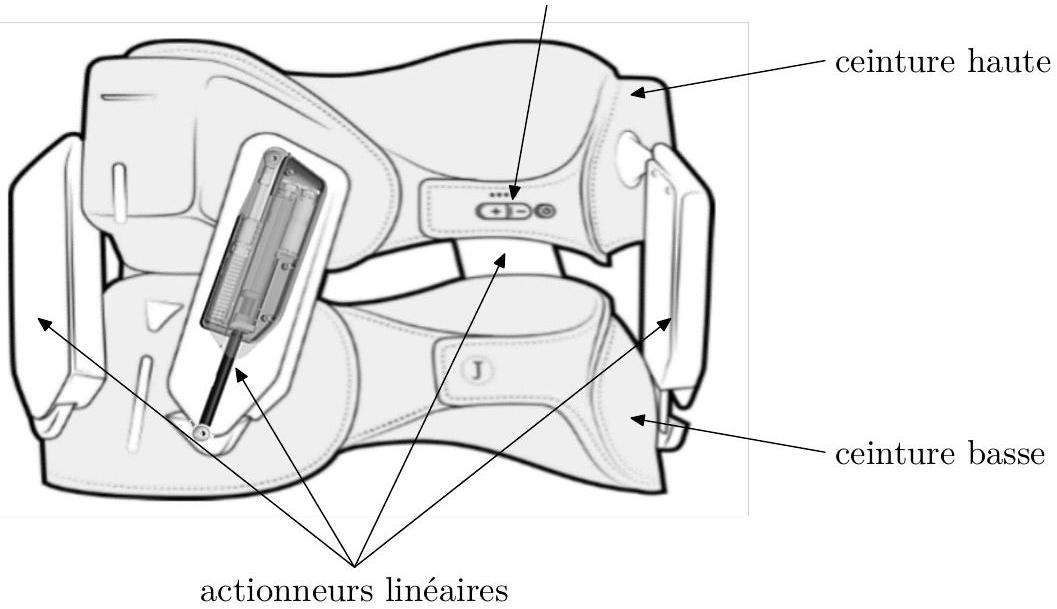
\includegraphics[width=\textwidth]{2025_09_16_5f2d7643f7e649c6833dg-01}
%\end{center}
%\end{figure}
%Figure 1 Exosquelette lombaire Japet



\begin{figure}[!h]
\centering
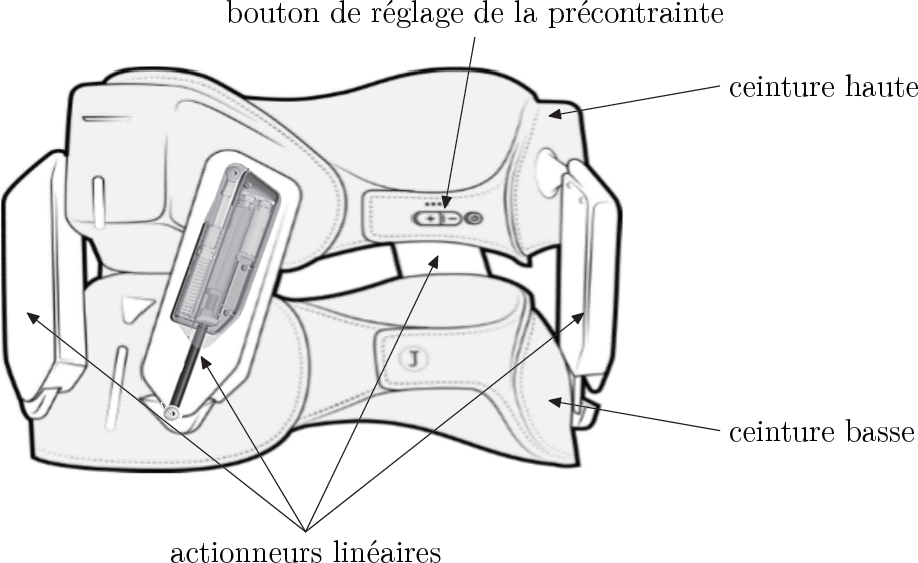
\includegraphics[width=.5\textwidth]{2023_mp_ccs_fig_01}
\caption{\label{ccs_mp_2023_fig_01}  Exosquelette lombaire Japet}
\end{figure}


Cet exosquelette lombaire est en priorité destiné au marché du travail et a vocation à soulager les salariés qui l'utilisent dans leurs mouvements quotidiens, en particulier dans les domaines de l'industrie ou de la logistique. Il est également destiné au soin de patients souffrant de lombalgie, en hôpital ou à domicile. Cet exosquelette n'a pas pour but d'augmenter les capacités physiques de l'être humain mais de les maintenir à un niveau satisfaisant. Cette assistance permet ainsi de conserver une activité professionnelle normale.

Grâce à l'effort de traction créé par les quatre actionneurs linéaires, le dispositif diminue la pression sur la colonne vertébrale afin de limiter la compression lombaire et soulager l'utilisateur des douleurs. Le système suit les mouvements de l'utilisateur en temps réel afin de conserver une liberté de mouvement totale et de préserver l'activité musculaire.

\subsection{Pré-dimensionnement des quatre actionneurs} %IB
\begin{obj}
Quantifier la force de traction à exercer par chaque actionneur linéaire pour atteindre un seuil de diminution de la pression intra-discale.
\end{obj}

La société Japet a développé un modèle numérique biomécanique (figure \ref{ccs_mp_2023_fig_02} à gauche) du corps humain permettant de déterminer la valeur de la force de traction à exercer par les actionneurs pour soulager les disques intervertébraux en diminuant la pression intra-discale.\\
Le modèle numérique biomécanique a permis d'obtenir les courbes de la figure \ref{ccs_mp_2023_fig_03} décrivant les évolutions des pressions intra-discales entre les vertèbres L3-L4 et L4-L5. Celles-ci ont été obtenues dans les conditions de simulation suivantes :

\begin{itemize}
  \item colonne vertébrale verticale ;
  \item chaque actionneur linéaire développe une force de traction progressivement de 0 à \SI{100}{N} ;
  \item l'évolution des forces de traction est lente afin de négliger les effets dynamiques.
\end{itemize}

%Q 1. \ref{ccs_mp_2023_q_}
\question{\label{ccs_mp_2023_q_01}
Après analyse des courbes de la figure \ref{ccs_mp_2023_fig_03}, justifier que la force de traction choisie par le constructeur, afin de limiter la pression intra-discale, est de 40 N par actionneur.}
\ifprof
\begin{corrige}
\end{corrige}
\else
\fi

%\begin{figure}[h]
%\begin{center}
%  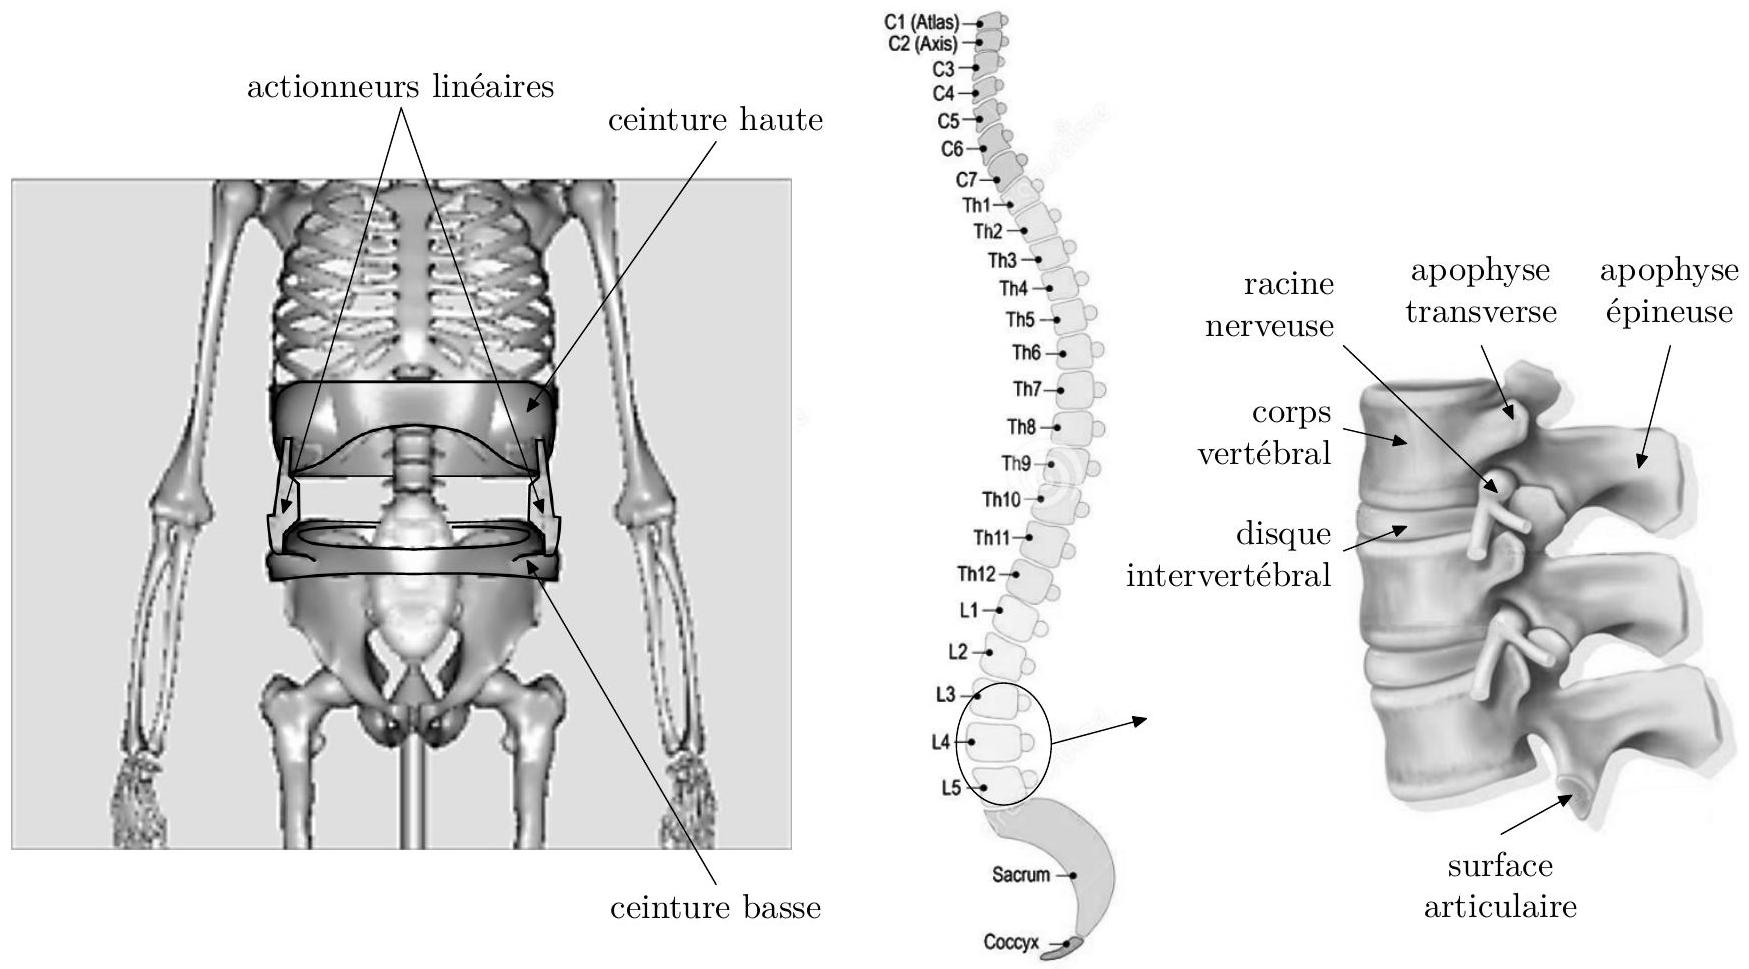
\includegraphics[width=\textwidth]{2025_09_16_5f2d7643f7e649c6833dg-02(1)}
%\captionsetup{labelformat=empty}
%\caption{Figure 2 Modèle numérique biomécanique (à gauche) et détail de la structure vertébrale avec numérotation des vertèbres (à droite)}
%\end{center}
%\end{figure}

\begin{figure}[!h]
\centering
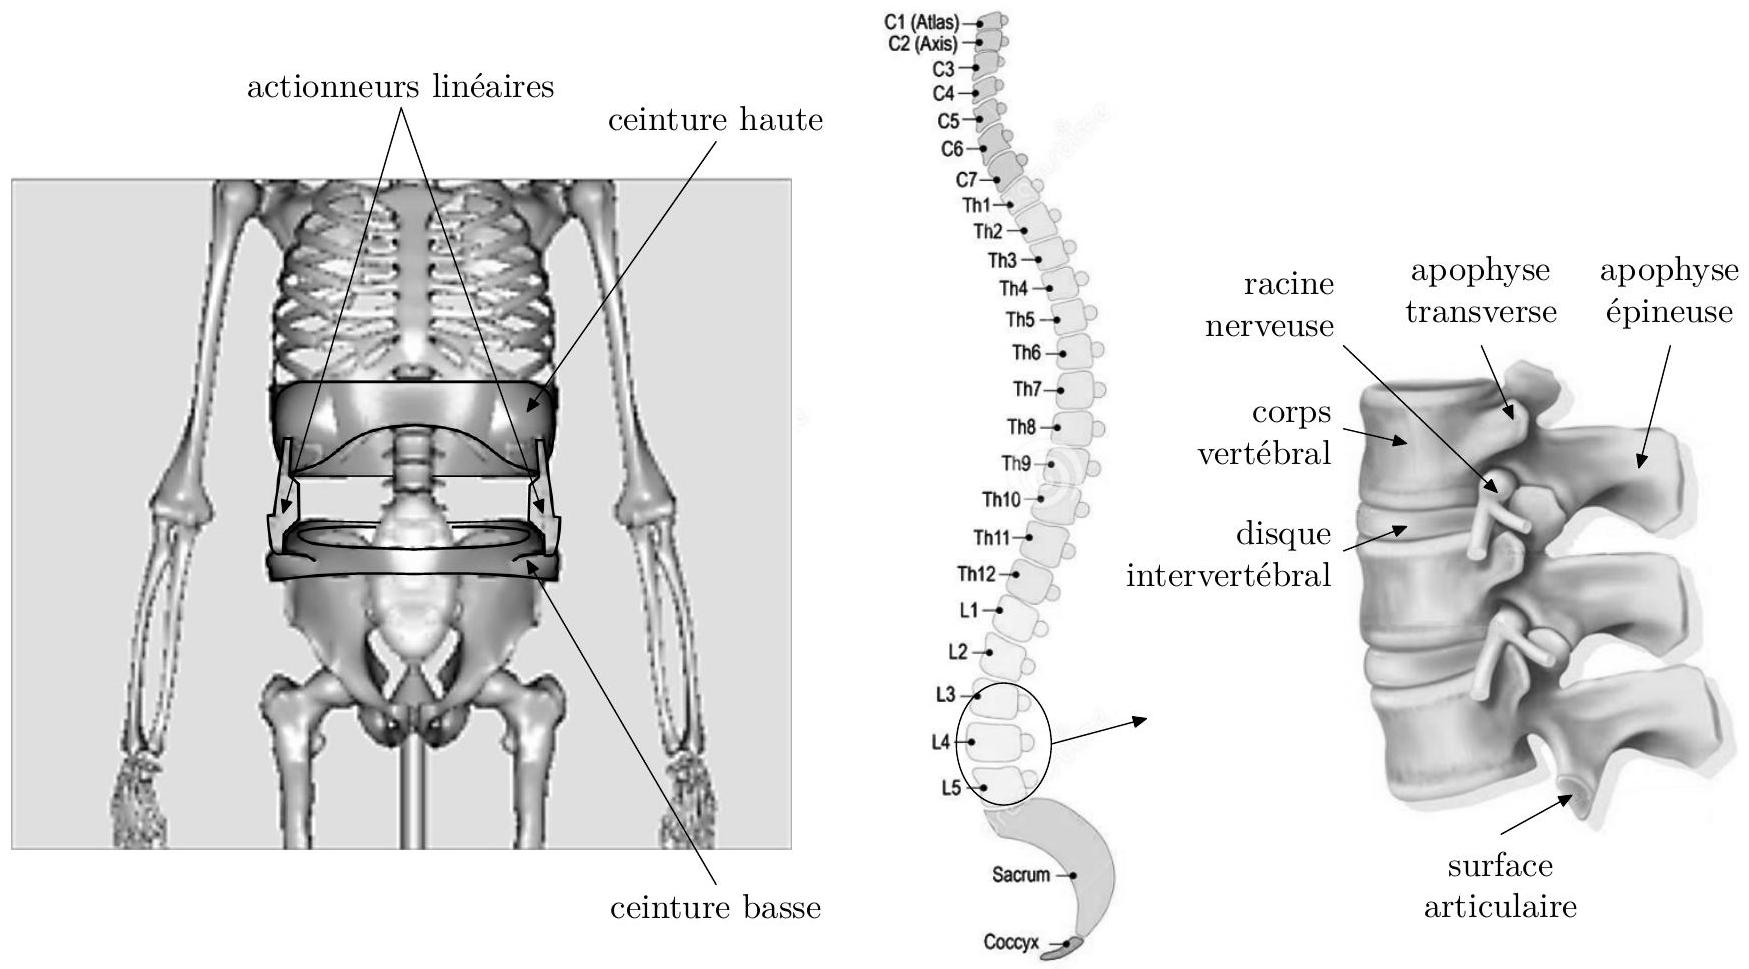
\includegraphics[width=\textwidth]{2025_09_16_5f2d7643f7e649c6833dg-02(1)}
\caption{\label{ccs_mp_2023_fig_02}  Modèle numérique biomécanique (à gauche) et détail de la structure vertébrale avec numérotation des vertèbres (à droite)}
\end{figure}



%
%\begin{figure}[h]
%\begin{center}
%  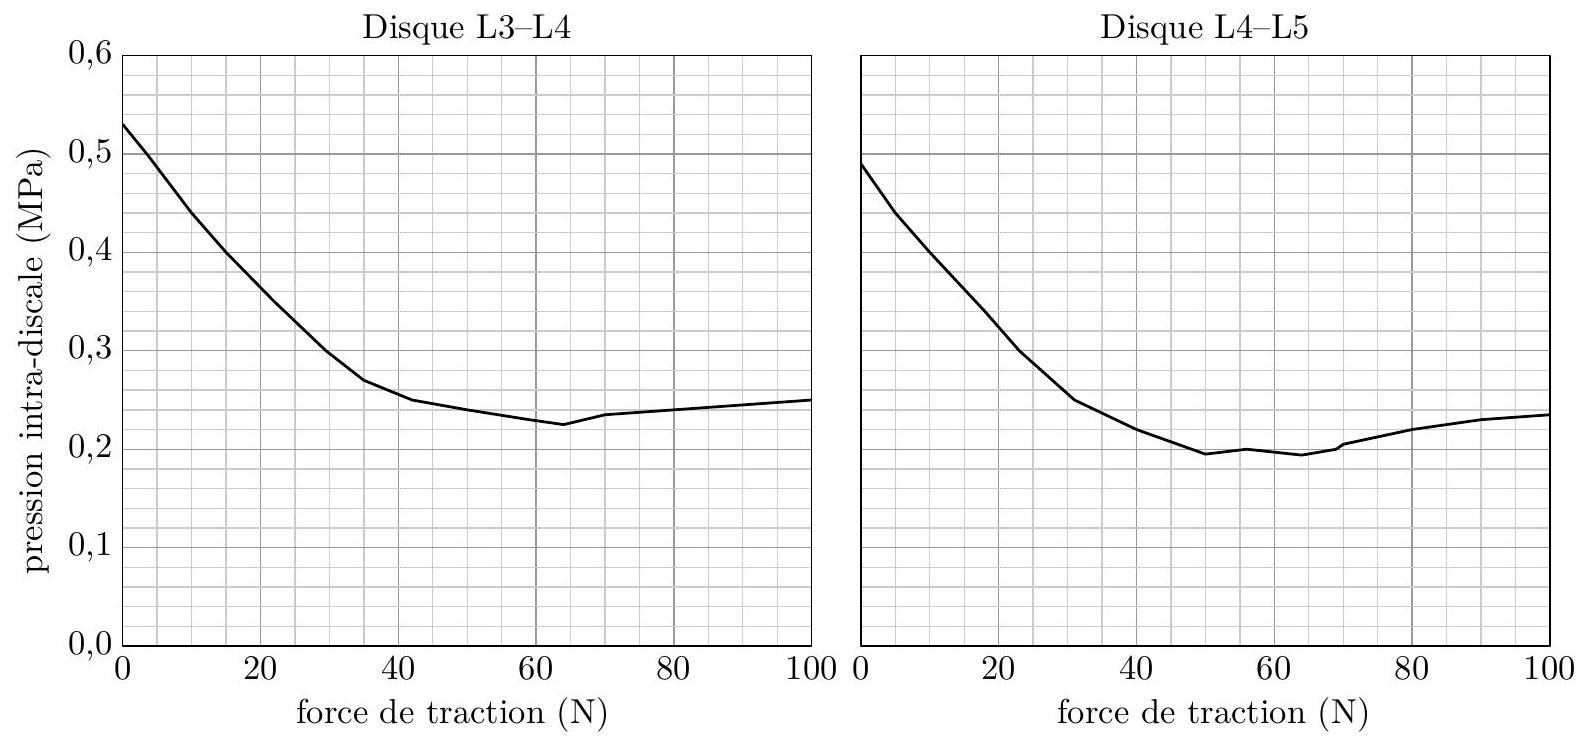
\includegraphics[width=\textwidth]{2025_09_16_5f2d7643f7e649c6833dg-02}
%\captionsetup{labelformat=empty}
%\caption{Figure 3 Évolution de la pression intra-discale simulée en L3-L4 et L4-L5 en fonction de la force de traction développée par un seul actionneur linéaire}
%\end{center}
%\end{figure}

\begin{figure}[!h]
\centering
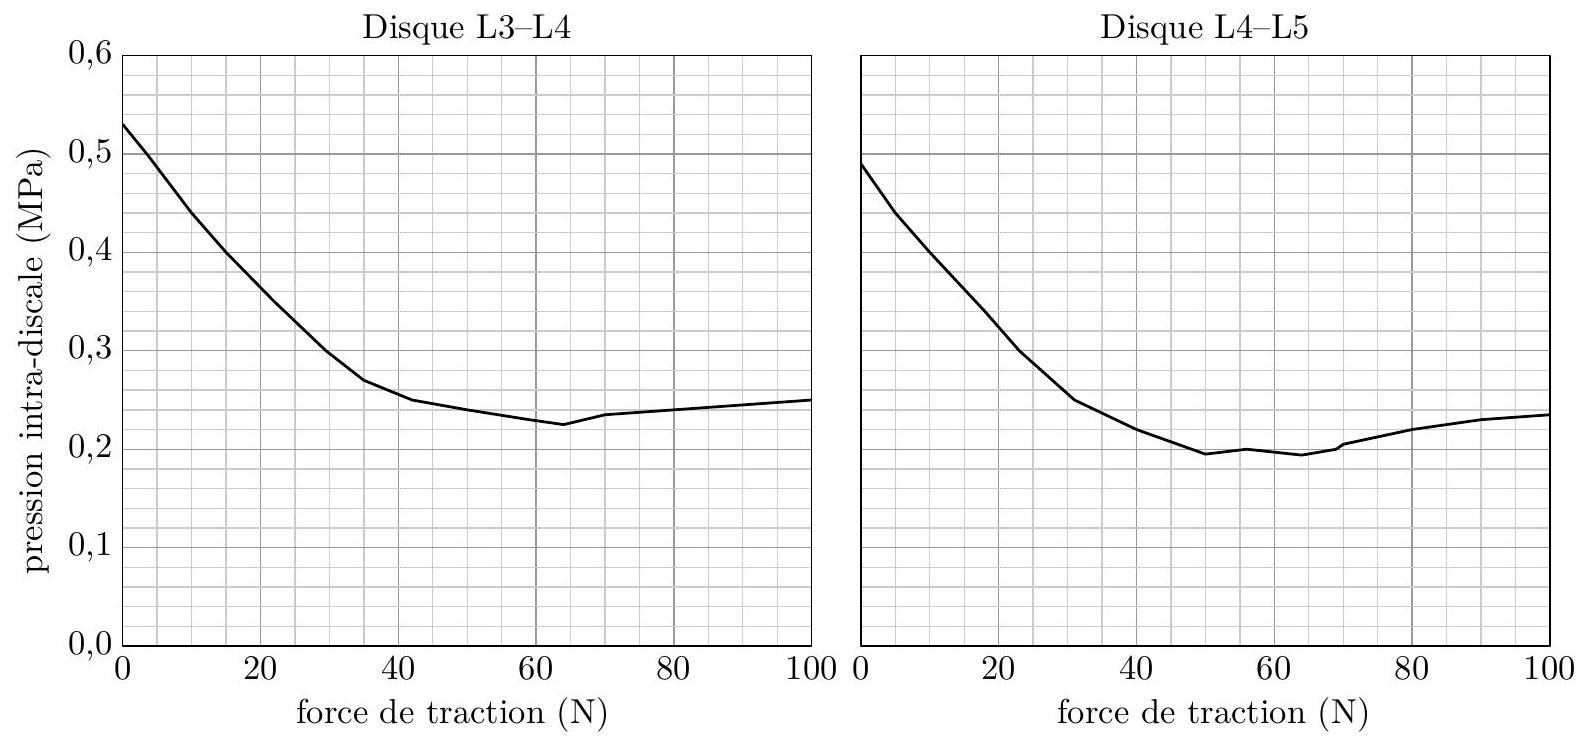
\includegraphics[width=\textwidth]{2025_09_16_5f2d7643f7e649c6833dg-02}
\caption{\label{ccs_mp_2023_fig_03}  Évolution de la pression intra-discale simulée en L3-L4 et L4-L5 en fonction de la force de traction développée par un seul actionneur linéaire}
\end{figure}




%IC
\subsection{Validation expérimentale du pré-dimensionnement des quatre actionneurs linéaires}
\begin{obj}
%Objectif\\
Montrer qu'il est possible de diminuer la pression intra-discale de 25 à $50 \%$ dans le cas d'une utilisation au quotidien de l'exosquelette.
\end{obj}

Des capteurs de pression ont été positionnés sur un cadavre (équipé de l'exosquelette Japet) dans le disque intervertébral L3-L4 en trois positions différentes du disque (avant, milieu, arrière) afin de mesurer la pression intra-discale réelle. Un effort de traction a été appliqué pour valider expérimentalement la baisse de pression intra-discale entre les vertèbres. Celles-ci ont été obtenues dans les conditions d'expérimentation suivantes :

\begin{itemize}
  \item à l'instant $t=0$, et pour une durée de 2 minutes, chaque actionneur linéaire développe une force de traction constante égale à \SI{40}{N} ;
  \item à l'instant $t=2 \mathrm{~min}$, les forces de traction sont annulées.
\end{itemize}

%\begin{figure}[h]
%\begin{center}
%  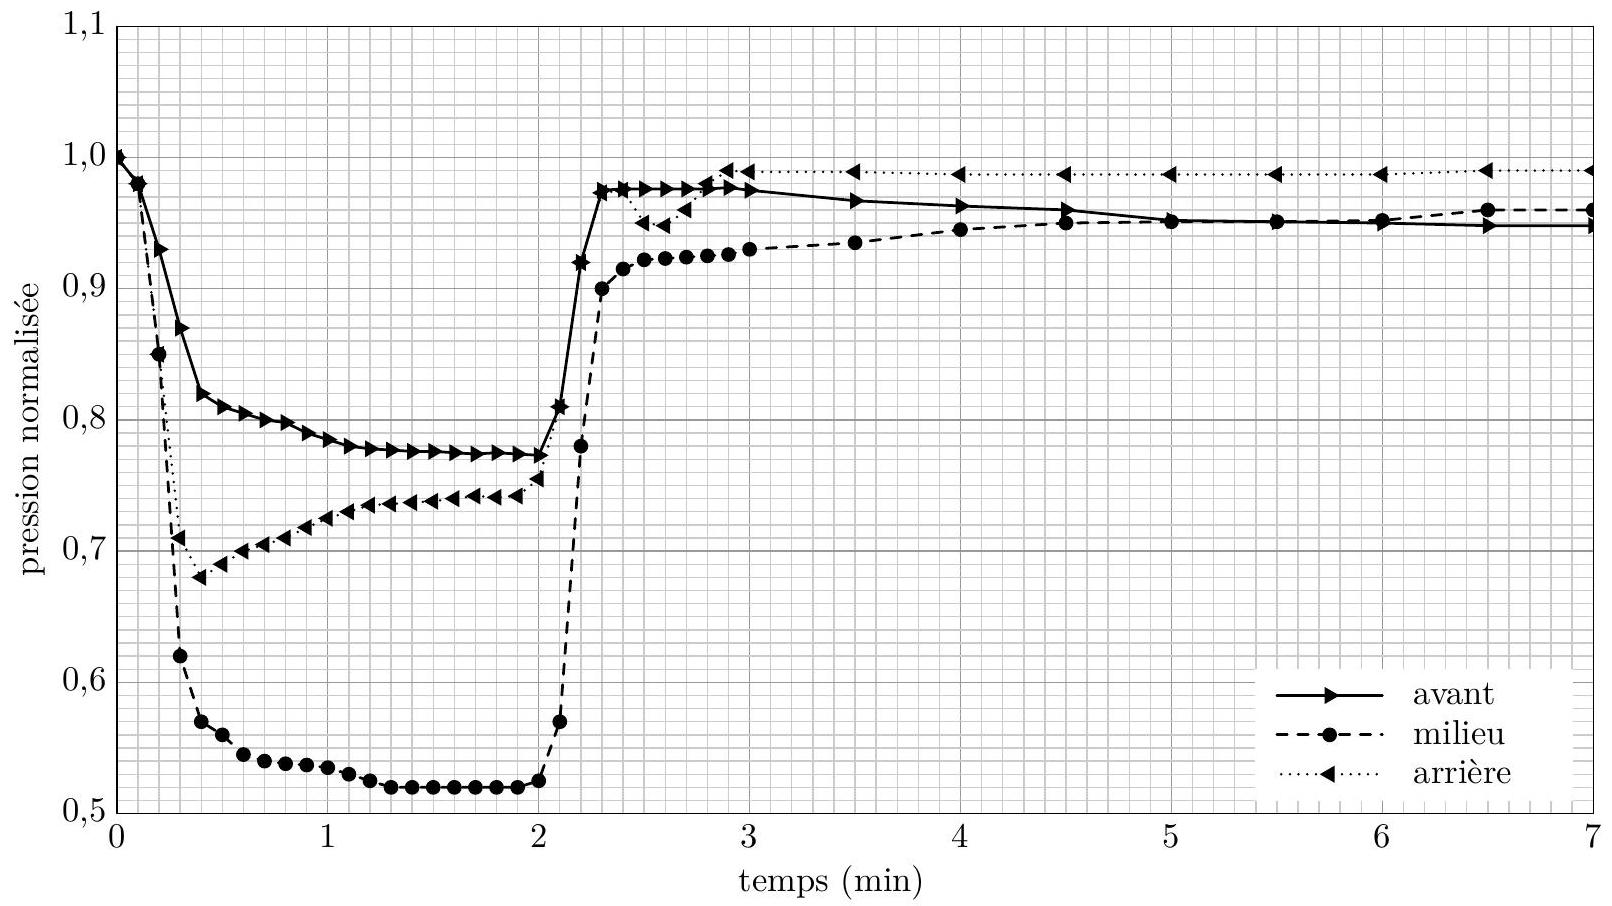
\includegraphics[width=\textwidth]{2025_09_16_5f2d7643f7e649c6833dg-03}
%\captionsetup{labelformat=empty}
%\caption{Figure 4 Évolution de la pression intra-discale mesurée et normalisée dans les trois positions du disque intervertébral L3-L4}
%\end{center}
%\end{figure}

\begin{figure}[!h]
\centering
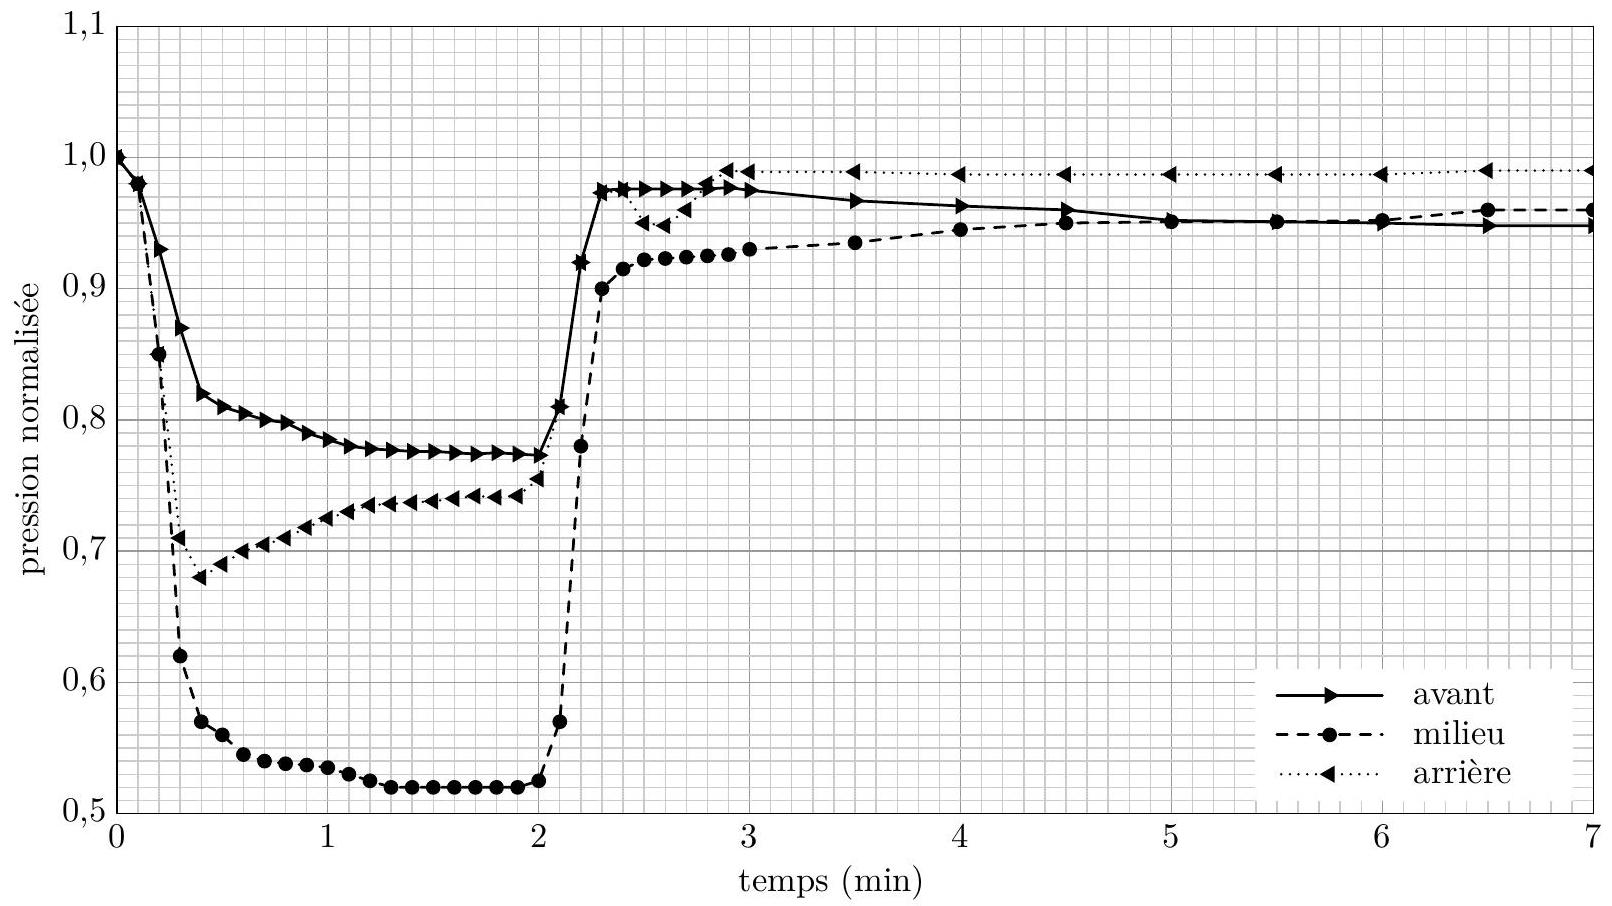
\includegraphics[width=\textwidth]{2025_09_16_5f2d7643f7e649c6833dg-03}
\caption{\label{ccs_mp_2023_fig_04}  Évolution de la pression intra-discale mesurée et normalisée dans les trois positions du disque intervertébral L3-L4}
\end{figure}



Les résultats ont été normalisés afin de tenir compte des conditions initiales ( $t<0$ ) en divisant les pressions mesurées par la pression intervertébrale initiale.\\

\question{\label{ccs_mp_2023_q_02}
Déterminer, pour les trois positions du capteur de pression dans le disque intervertébral L3-L4, la diminution moyenne de la pression intra-discale (en \%) pendant les deux minutes d'application de l'effort de traction, sans prendre en compte la phase transitoire de 0 à $0,5 \mathrm{~min}$.}
\ifprof
\begin{corrige}
\end{corrige}
\else
\fi


Cette pré-étude théorique ainsi que la validation expérimentale permettent de montrer l'efficacité du soulagement intra-discal par un système externe actif. Le développement de l'exosquelette est basé sur ces résultats. L'analyse des résultats des expérimentations décrites précédemment a permis de définir le cahier des charges partiel proposé dans le tableau \ref{ccs_mp_2023_tab_01}.

\begin{table}[h]
\begin{center}
\begin{tabular}{lp{5cm}p{5cm}p{3cm}p{2.5cm}}
\hline
\textbf{Id} & \textbf{Exigence} & \textbf{Critère} & \textbf{Niveau} & \textbf{Flexibilité} \\
\hline
\multirow[t]{2}{*}{Id1} & \multirow[t]{2}{4cm}{Limiter la compression lombaire pour soulager les douleurs} & Force de traction pour chaque actionneur linéaire & 40 N & $< \pm 2,5 \%$ \\
 &  & Vitesse maximale de la montée de la force de traction & $100 \mathrm{~N} \cdot \mathrm{~s}^{-1}$ & nulle \\
\hline
Id2 & Préserver l'activité musculaire, en garantissant la liberté de mouvement naturel du corps humain & Liberté totale de mouvement entre les ceintures basse et haute & 6 degrés de liberté & aucune \\
\hline
\end{tabular}
%\captionsetup{labelformat=empty}
\caption{Extrait du cahier des charges fonctionnel de l'exosquelette \label{ccs_mp_2023_tab_01}}
\end{center}
\end{table}

%I.D - 
\subsection{Problématique et organisation de l'étude}
L'exosquelette lombaire, répertorié comme un système médical par les autorités de santé, doit garantir un fonctionnement sûr afin de ne causer aucun dommage à la colonne vertébrale tout en assurant une traction au niveau des vertèbres pour soulager les disques intervertébraux. Le mouvement naturel du corps devra être conservé. Ceci implique que l'amplitude des mouvements de l'exosquelette lombaire devra s'adapter aux mouvements du corps et que l'effort d'assistance devra correspondre aux valeurs définies dans le cahier des charges partiel.

La problématique globale du sujet est de valider un modèle de connaissance simulant la capacité des actionneurs linéaires à exercer un effort de traction maitrisé tout en garantissant la liberté de mouvement naturel du corps humain.\\
L'étude est limitée au mouvement de l'ensemble dans le plan sagittal (figure \ref{ccs_mp_2023_fig_05}). Pour aborder la problématique, l'étude s'intéresse à :

\begin{itemize}
  \item un degré de liberté particulier de la ceinture haute par rapport à la ceinture basse ;
  \item la capacité d'un actionneur linéaire à exercer une force de \SI{40}{N}.
\end{itemize}

%\begin{figure}[h]
%\begin{center}
%  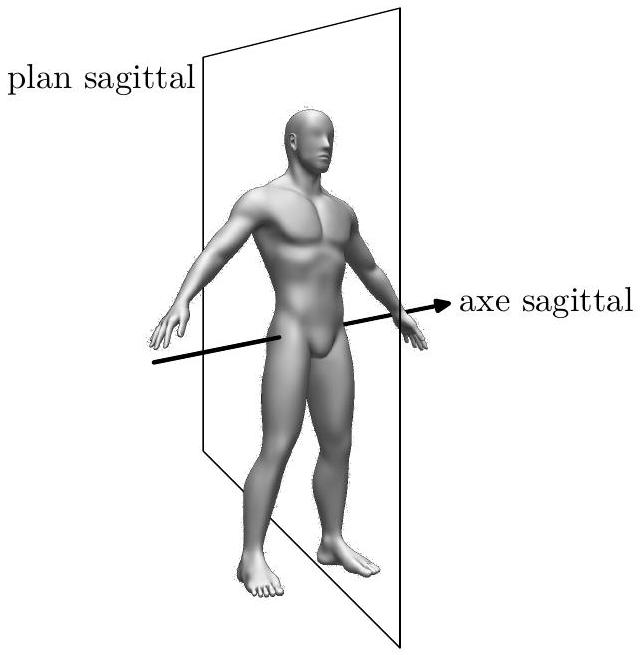
\includegraphics[width=\textwidth]{2025_09_16_5f2d7643f7e649c6833dg-04}
%\captionsetup{labelformat=empty}
%\caption{Figure 5 Plan et axe sagittal}
%\end{center}
%\end{figure}

\begin{figure}[!h]
\centering
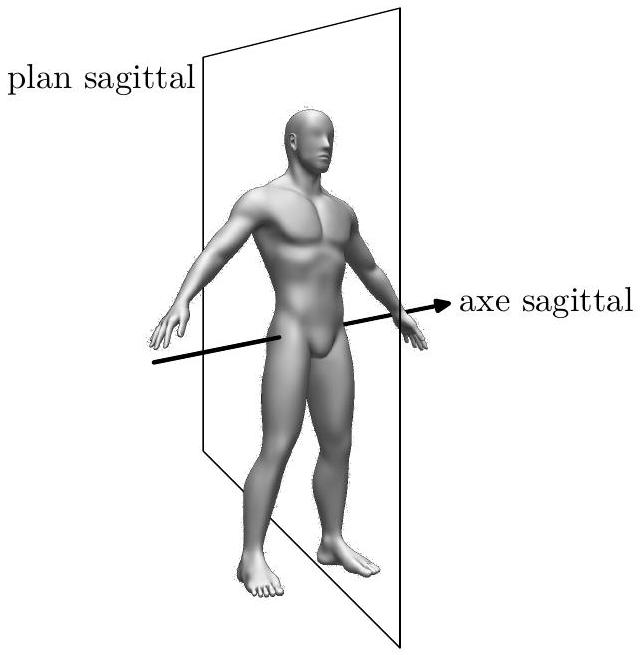
\includegraphics[width=.4\textwidth]{2025_09_16_5f2d7643f7e649c6833dg-04}
\caption{\label{ccs_mp_2023_fig_05}  Plan et axe sagittal}
\end{figure}


Après avoir déterminé l'amplitude nécessaire du déplacement des actionneurs linéaires, l'étude portera sur la caractérisation dynamique et la commande d'un des quatre actionneurs linéaires. Cette dernière nécessite l'élaboration d'un modèle de connaissance du système étudié. La société Japet a construit un banc d'essai et de mesure. Ce banc d'essai a pour finalité de :

\begin{itemize}
  \item contrôler l'amplitude nécessaire du déplacement des actionneurs linéaires ;
  \item comparer les résultats issus des simulations aux résultats expérimentaux pour une position particulière d'un actionneur linéaire, dans un premier temps.\\
Par la suite, le constructeur validera chaque actionneur linéaire commercialisé à l'aide du banc d'essai dans une démarche qualité.
\end{itemize}

\section{Étude de l'amplitude du déplacement de l'actionneur pour conserver un mouvement naturel} % II 
%\section{Objectif}
\begin{obj}
Déterminer la course des actionneurs permettant de suivre les mouvements du corps conformément à l'exigence Id2 du cahier des charges partiel.
\end{obj}


L'exigence Id2 «~Préserver l'activité musculaire~» est composée de deux exigences Id2.1 et Id2.2 (tableau \ref{ccs_mp_2023_tab_02}). Le fonctionnement de l'exosquelette nécessite une mise en précontrainte. Pour cette mise en précontrainte, chaque actionneur linéaire doit exercer une force de \SI{40}{N}. Cette valeur est obtenue par déplacement vertical de la ceinture haute par rapport à la ceinture basse.

\begin{table}[h]
\begin{center}
\begin{tabular}{|l|p{4cm}|p{4cm}|l|l|}
\hline
Id & Exigence & Critère & Niveau & Flexibilité \\
\hline
Id2.1 & Permettre le mouvement de translation de la ceinture haute par rapport à la ceinture basse & Déplacement vertical $\Delta h$ de la ceinture haute par rapport à la ceinture basse & $\Delta h=50 \mathrm{~mm}$ & < 10 \% \\
\hline
Id2.2 & Permettre le mouvement de rotation de la ceinture haute par rapport à la ceinture basse & Amplitude de rotation $\varphi$ & [ $0,+20^{\circ}$ ] selon l'axe sagittal & < 10 \% \\
\hline
\end{tabular}
%\captionsetup{labelformat=empty}
\caption{\label{ccs_mp_2023_tab_02}Extrait du cahier des charges fonctionnel limité au mouvement dans le plan sagittal de l'exosquelette}
\end{center}
\end{table}

\subsection{Analyse des exigences 2.1 et 2.2} % Ajout XP

L'exigence Id2.1 correspond à la valeur du déplacement vertical nécessaire à la précontrainte. Cette valeur est propre à chaque utilisateur. Dans le cas extrême, cette valeur correspond à un déplacement vertical de \SI{50}{mm}. L'étude cinématique est limitée à un mouvement de flexion avant. La figure \ref{ccs_mp_2023_fig_06} décrit le mouvement ainsi que le positionnement de l'exosquelette dans le plan sagittal. La figure \ref{ccs_mp_2023_fig_07} décrit le modèle géométrique paramétré de l'exosquelette. La liaison sphère-cylindre en $C$ modélise les degrés de liberté supprimés par les éléments extérieurs au système (colonne vertébrale + tissus mous).\\

\question{\label{ccs_mp_2023_q_03}
Déterminer l'expression de la longueur $l_{2}(t)$ en fonction de $\varphi(t), h(t), b$ et $a$.}
\ifprof
\begin{corrige}
\end{corrige}
\else
\fi


%\begin{figure}[h]
%\begin{center}
%  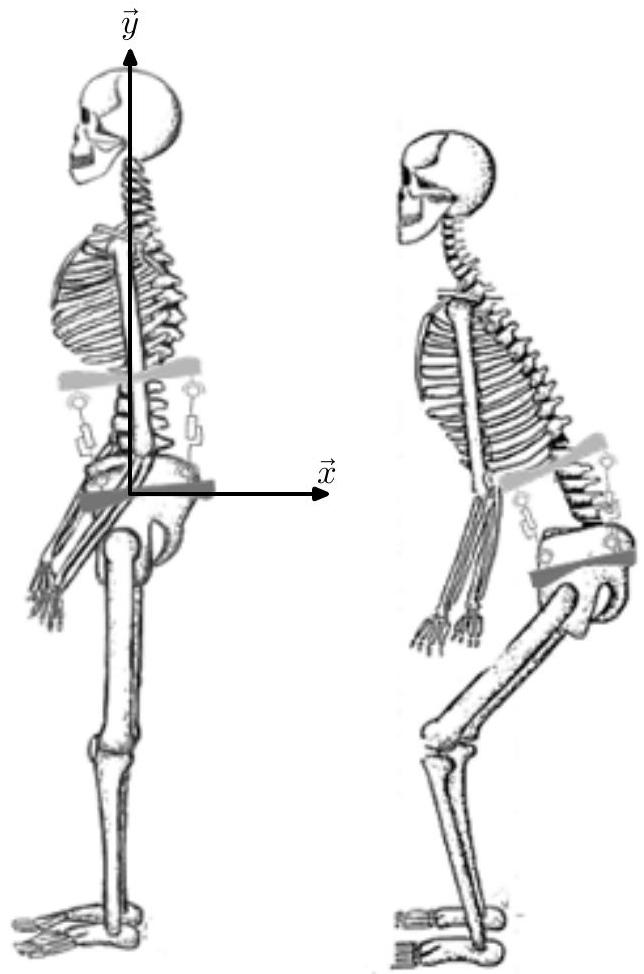
\includegraphics[width=\textwidth]{2025_09_16_5f2d7643f7e649c6833dg-05}
%\captionsetup{labelformat=empty}
%\caption{Figure 6 Mouvement de flexion et implantation de l'exosquelette}
%\end{center}
%\end{figure}


\begin{figure}[!h]
\centering
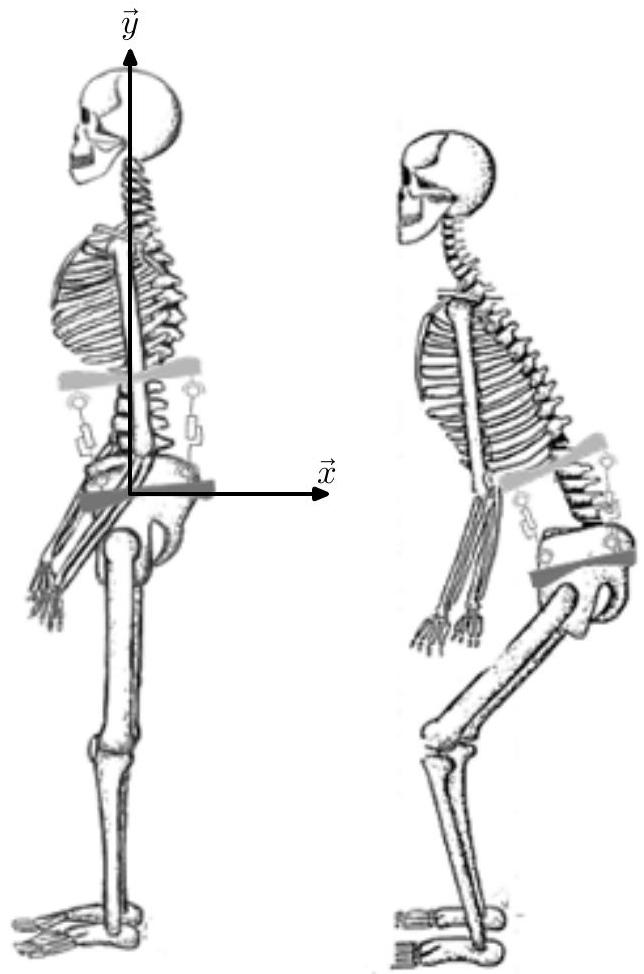
\includegraphics[width=.4\textwidth]{2025_09_16_5f2d7643f7e649c6833dg-05}
\caption{\label{ccs_mp_2023_fig_06}  Mouvement de flexion et implantation de l'exosquelette}
\end{figure}



%\begin{figure}[h]
%\begin{center}
%  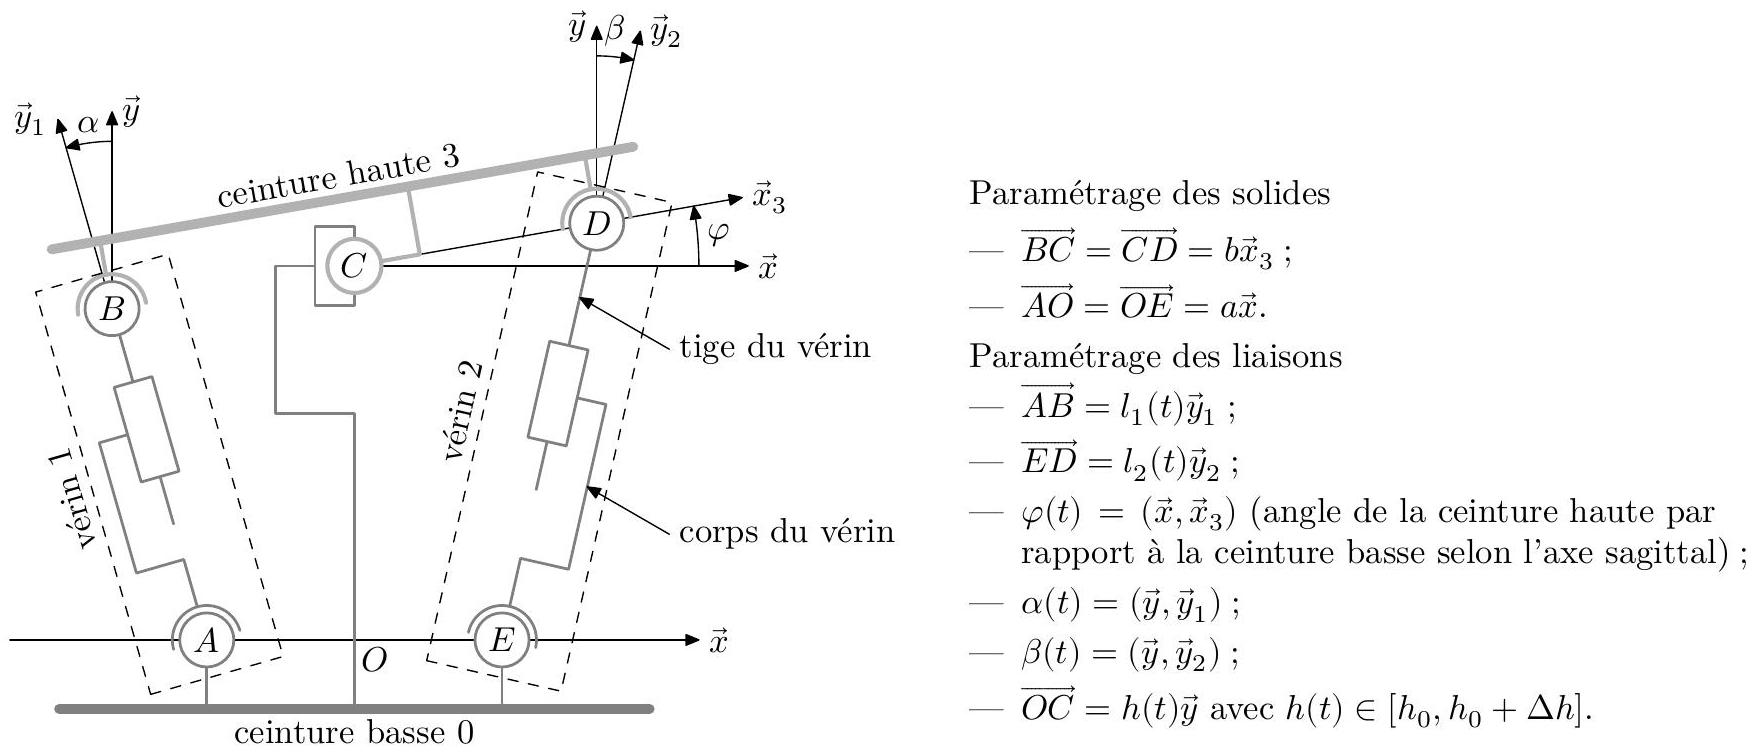
\includegraphics[width=\textwidth]{2025_09_16_5f2d7643f7e649c6833dg-05(1)}
%\captionsetup{labelformat=empty}
%\caption{Figure 7 Paramétrage cinématique}
%\end{center}
%\end{figure}


\begin{figure}[!h]
\centering
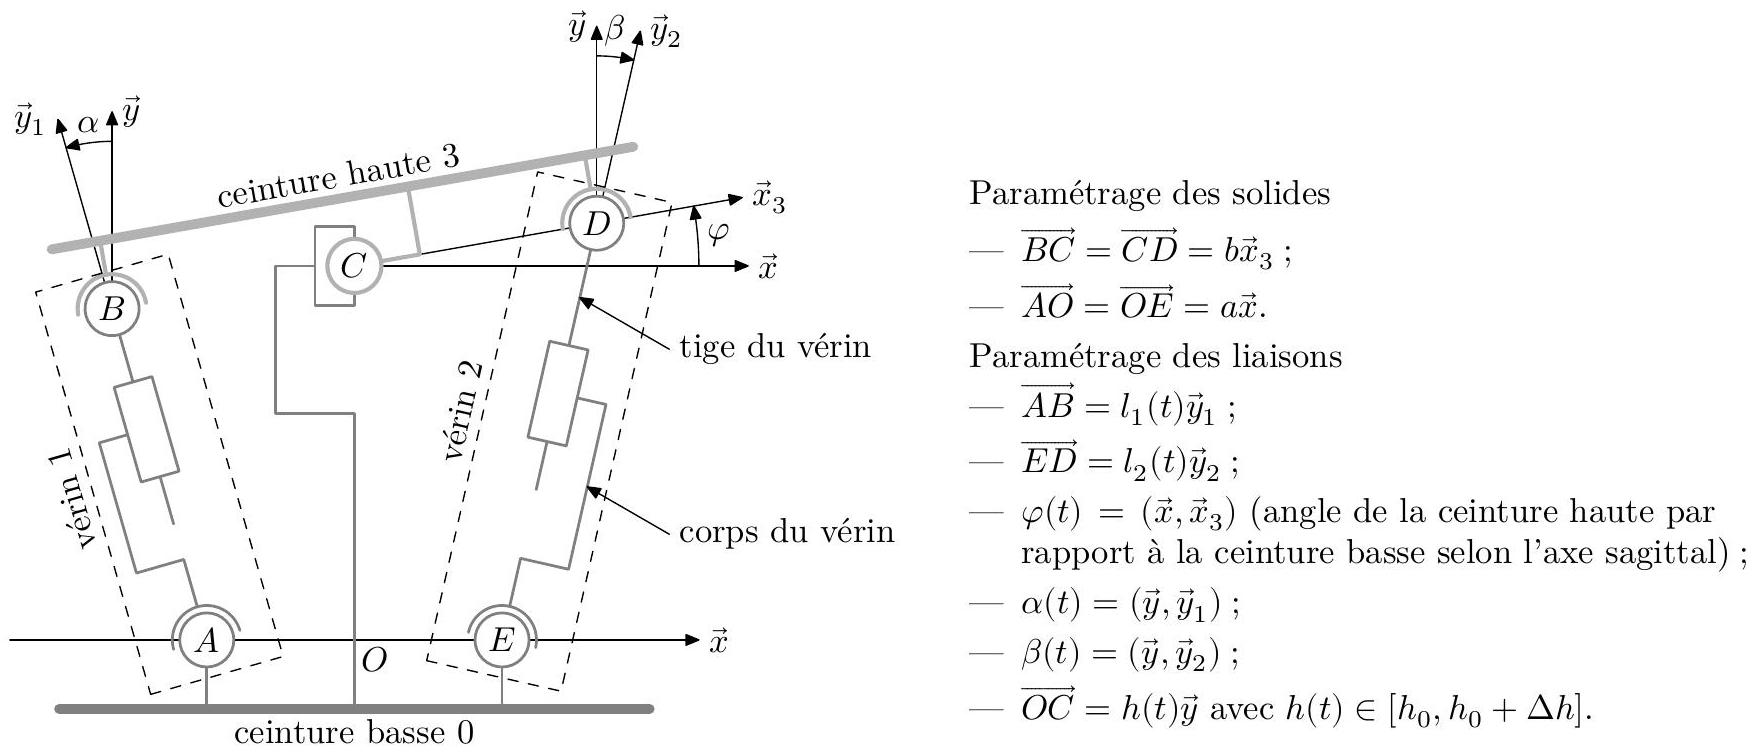
\includegraphics[width=\textwidth]{2025_09_16_5f2d7643f7e649c6833dg-05(1)}
\caption{\label{ccs_mp_2023_fig_07} Paramétrage cinématique }
\end{figure}




Le protocole de mise en précontrainte et d'utilisation de l'exosquelette est le suivant:

\begin{enumerate}
  \item à $t=0$, mise en place de l'ensemble en ajustant sur le corps de l'usager les deux ceintures basse et haute $\left(h_{0}=h(0)\right)$;
  \item pour $t \in[0, T]$, mise en précontrainte $\left(h(T)=h_{0}+\Delta h\right)$;
  \item pour $t>T$, mouvement libre (dans notre étude, $\varphi(t)$ est limité de $0^{\circ}$ à $20^{\circ}$ selon l'axe sagittal).
\end{enumerate}

On définit la course d'un actionneur linéaire comme étant la distance que peut parcourir la tige par rapport au corps entre ses positions extrêmes.\\

%Q 4. 
\question{\label{ccs_mp_2023_q_04}
Le point $C$ restant sur l'axe $\axe{O}{y}$, déterminer la course du vérin 2 à partir du protocole défini précédemment pour les valeurs $a=100 \mathrm{~mm}, b=150 \mathrm{~mm}, h_{0}=100 \mathrm{~mm}$ et $\Delta h=50 \mathrm{~mm}$.}
\ifprof
\begin{corrige}
\end{corrige}
\else
\fi


Une étude équivalente montre que la course du vérin 2 est supérieure à celle du vérin 1 .

La course obtenue permet donc de dimensionner géométriquement les actionneurs en fonction des positions des points d'accroche sur les ceintures haute et basse. On peut ainsi définir la valeur de contrôle à mettre en place sur le banc d'essai. Cette valeur est vérifiée pour chaque actionneur fabriqué.\\
L'exigence sur la liberté de mouvement angulaire étant vérifiée, la suite de l'étude a pour but de caractériser la dynamique et la commande d'un des quatre actionneurs ce qui nécessite l'élaboration d'un modèle de connaissance. La validation sera faite à partir des résultats de la force de traction mesurée sur le banc d'essai.


%%%% DEBUT AJOUT %%%
\subsection{Analyse de la structure cinématique de l'exosquelette} % Ajout XP

\question{Tracer le graphe des liaisons associé au modèle d'exosquelette proposé figure \ref{ccs_mp_2023_fig_07}.}

\question{\text{Sans calcul}, proposer une méthode permettant de déterminer la liaison équivalente entre la ceinture basse \textbf{0} et la ceinture haute \textbf{3}.}






\section{Élaboration du modèle de connaissance d'un actionneur linéaire placé sur un banc d'essai}% III
%III.A - 
\subsection{Étude de la dynamique de l'actionneur linéaire dans le cas particulier représentatif de la mise en précontrainte étudiée à la question \ref{ccs_mp_2023_q_03} modélisant le système dans cette configuration particulière}

\begin{obj}
Définir un modèle de connaissance de la dynamique du système permettant d'obtenir les équations d'un modèle de simulation comparable aux mesures du banc d'essai.
\end{obj}

Le système est placé sur un banc d'essai en position horizontale (figure \ref{ccs_mp_2023_fig_08}). Dans cette configuration, la pesanteur est portée par la direction $\vec{z}_{0}$. On rappelle que le banc fonctionne selon deux protocoles distincts

\begin{itemize}
  \item vérification de la course définie précédemment (non étudiée ici) ;
  \item vérification de la force exercée par un actionneur linéaire pour effectuer la précontrainte.
\end{itemize}

%\begin{figure}[h]
%\begin{center}
%  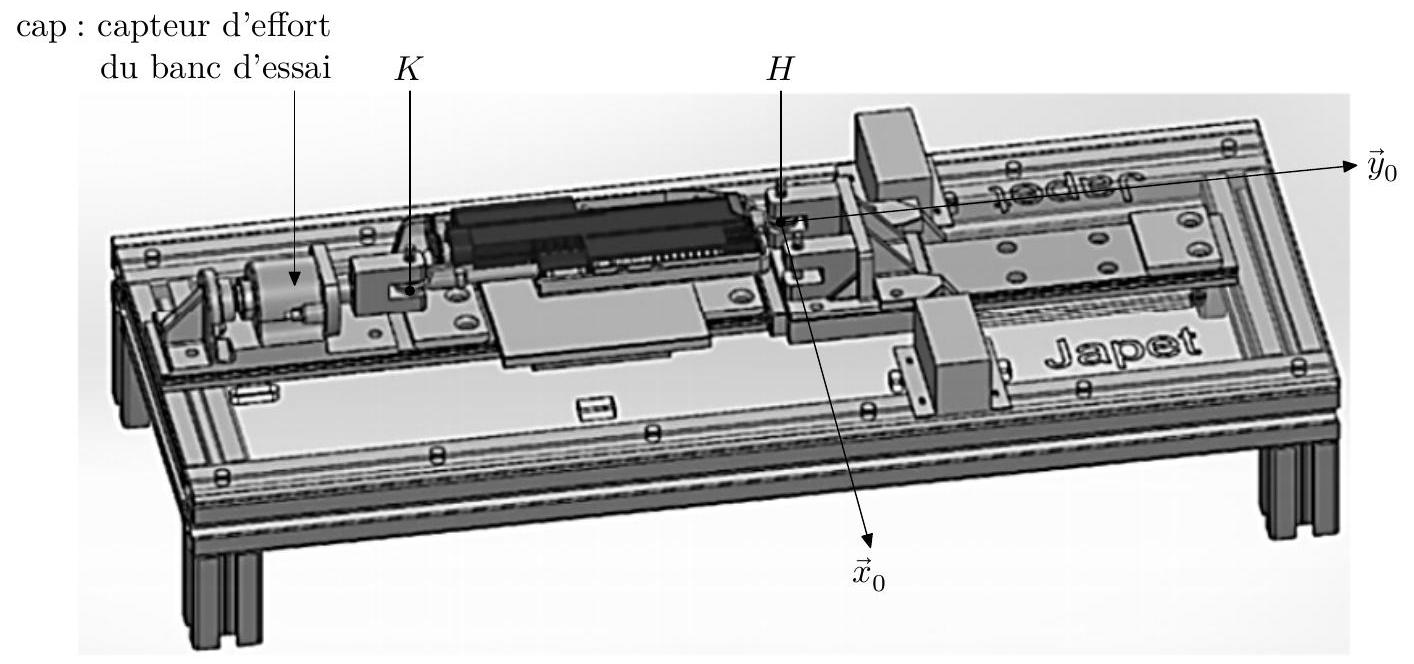
\includegraphics[width=\textwidth]{2025_09_16_5f2d7643f7e649c6833dg-06(1)}
%\captionsetup{labelformat=empty}
%\caption{Figure 8 Banc d'essai}
%\end{center}
%\end{figure}


\begin{figure}[!h]
\centering
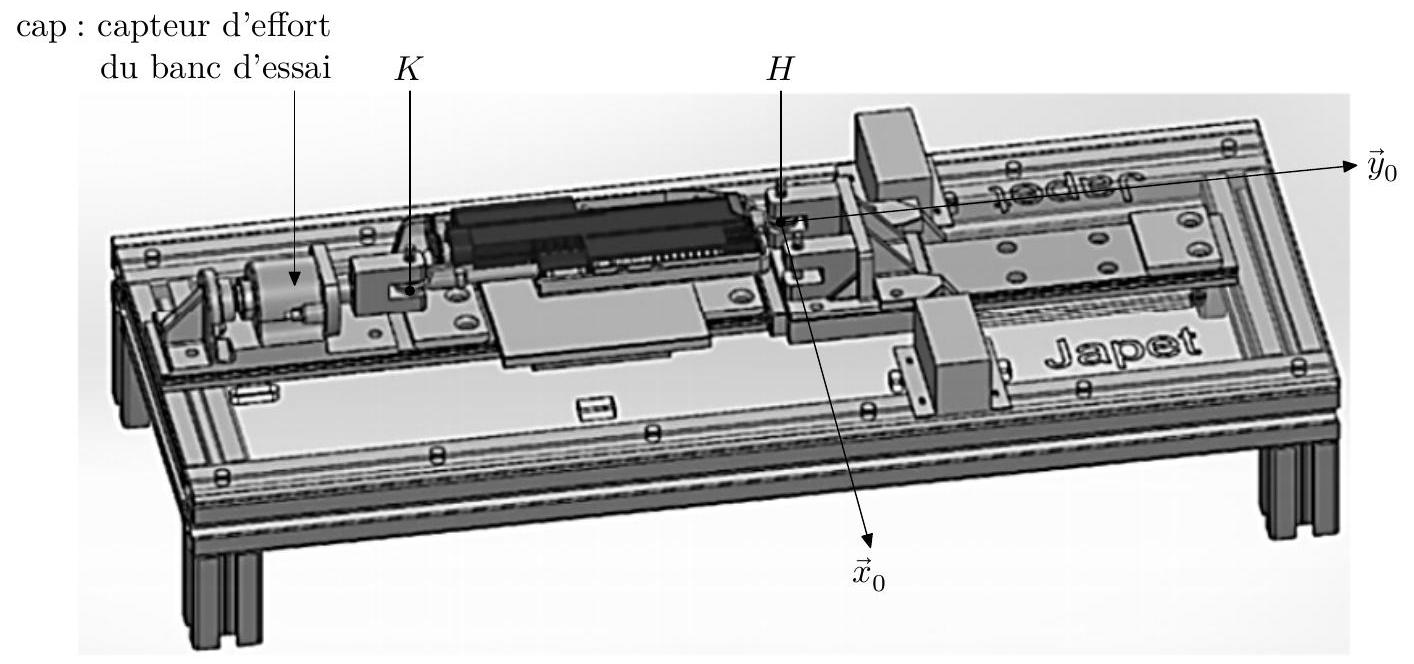
\includegraphics[width=.8\textwidth]{2025_09_16_5f2d7643f7e649c6833dg-06(1)}
\caption{\label{ccs_mp_2023_fig_08}  Banc d'essai}
\end{figure}



Pour la vérification de la force de précontrainte, l'actionneur linéaire est bloqué en $H$ et un capteur d'effort, noté cap (figure \ref{ccs_mp_2023_fig_08}), supposé indéformable, est placé en $K$. Cette configuration permet uniquement de valider la performance relative à la mise en précontrainte.\\
La raideur du ressort du capteur d'effort de l'actionneur linéaire (figure \ref{ccs_mp_2023_fig_09}) a été choisie à partir d'une campagne d'essais réalisée par différents utilisateurs qui ont exprimé leur ressenti en donnant une note de confort. L'exploitation des données recueillies a permis au fabricant de déterminer le meilleur compromis parmi les retours des différents utilisateurs.

Chaine d'action : transmission de l'énergie par une chaine moteur-réducteur-vis-écrou

%\begin{figure}[h]
%\begin{center}
%  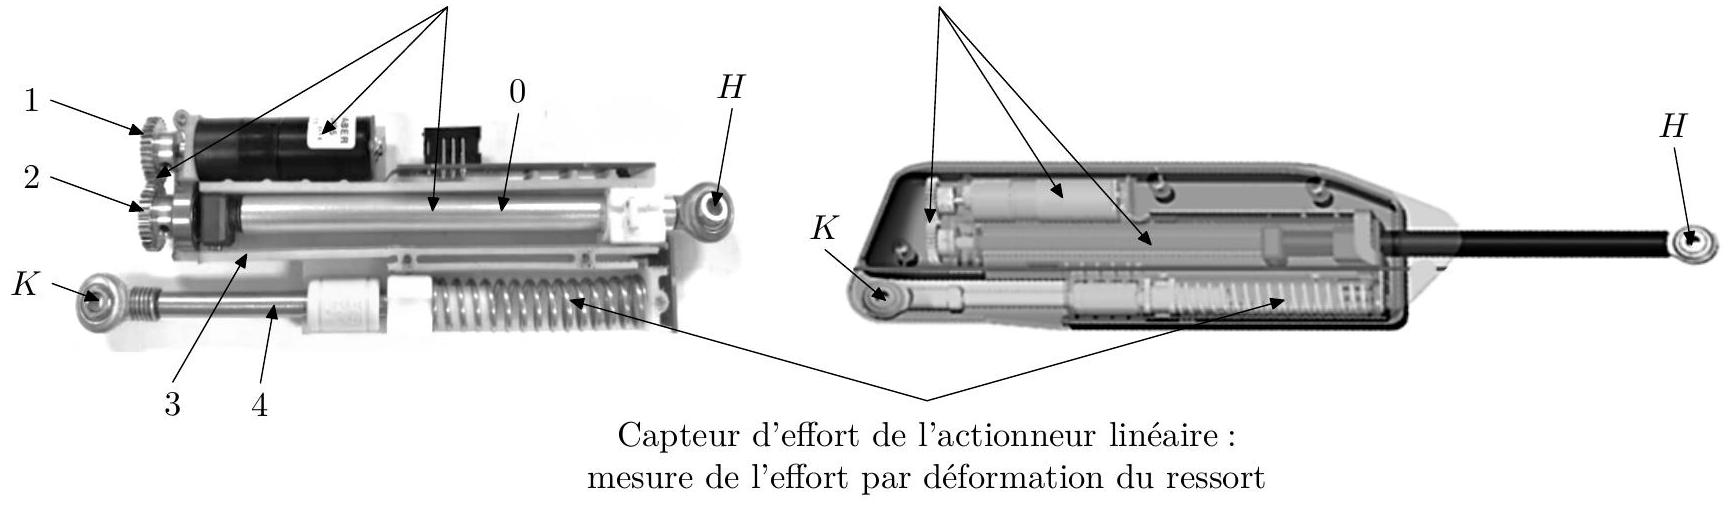
\includegraphics[width=\textwidth]{2025_09_16_5f2d7643f7e649c6833dg-06}
%\captionsetup{labelformat=empty}
%\caption{Figure 9 Actionneur linéaire}
%\end{center}
%\end{figure}


\begin{figure}[!h]
\centering
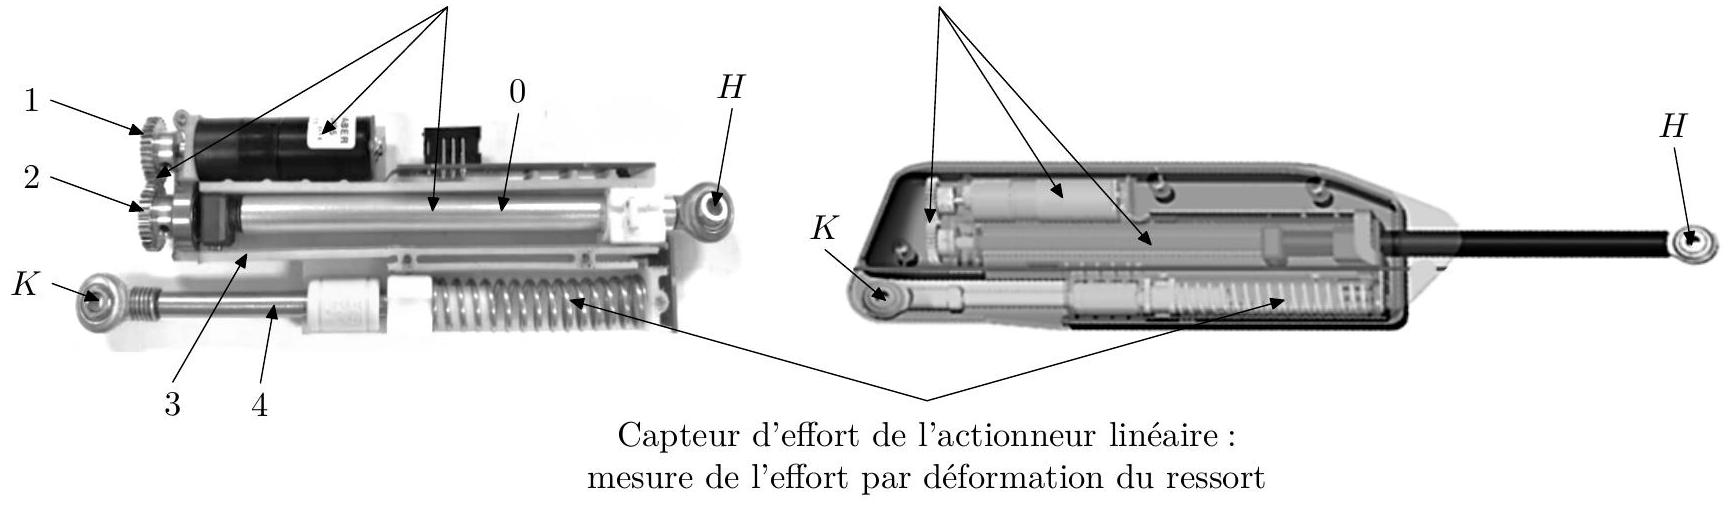
\includegraphics[width=\textwidth]{2025_09_16_5f2d7643f7e649c6833dg-06}
\caption{\label{ccs_mp_2023_fig_09} Actionneur linéaire }
\end{figure}


Dans la configuration spécifique retenue, les points $K$ et $H$ sont immobiles par rapport au châssis du banc d'essai. Les solides (0) et (4) sont immobiles par rapport au châssis du banc d'essai. L'action mécanique de l'actionneur linéaire sur le capteur d'effort du banc d'essai est un glisseur de support passant par $K$ et de résultante $\vec{F}_{4 \rightarrow \text { cap }}$. Le capteur du banc d'essai mesure ainsi $\vec{F}_{4 \rightarrow \text { cap }} \cdot \vec{y}_{0}$. On suppose que c'est une image fidèle de la force de traction exercée par l'actionneur linéaire.

%\begin{figure}[h]
%\begin{center}
%  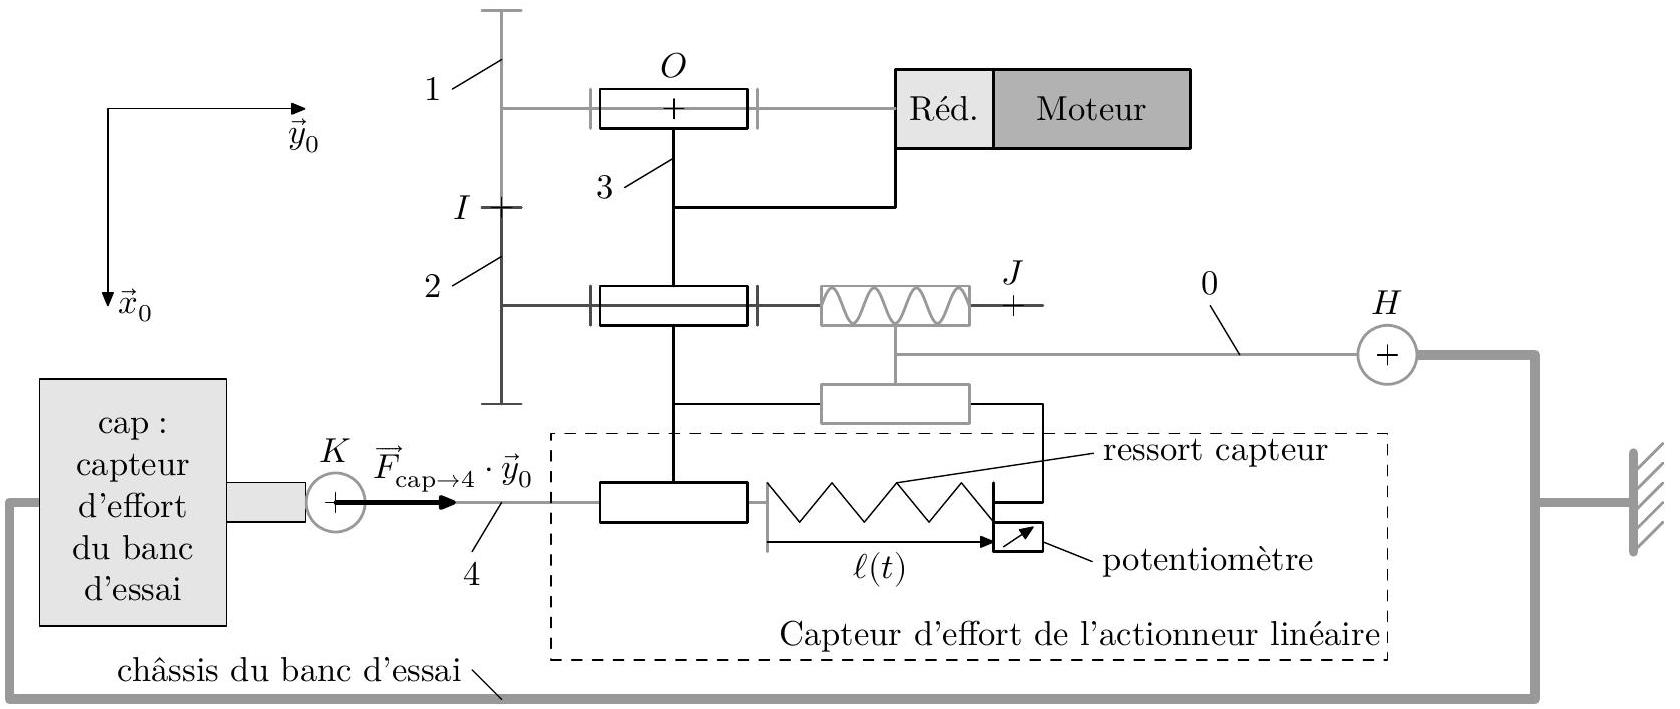
\includegraphics[width=\textwidth]{2025_09_16_5f2d7643f7e649c6833dg-07}
%\captionsetup{labelformat=empty}
%\caption{Figure 10 Modèle d'étude de l'actionneur linéaire sur le banc d'essai}
%\end{center}
%\end{figure}


\begin{figure}[!h]
\centering
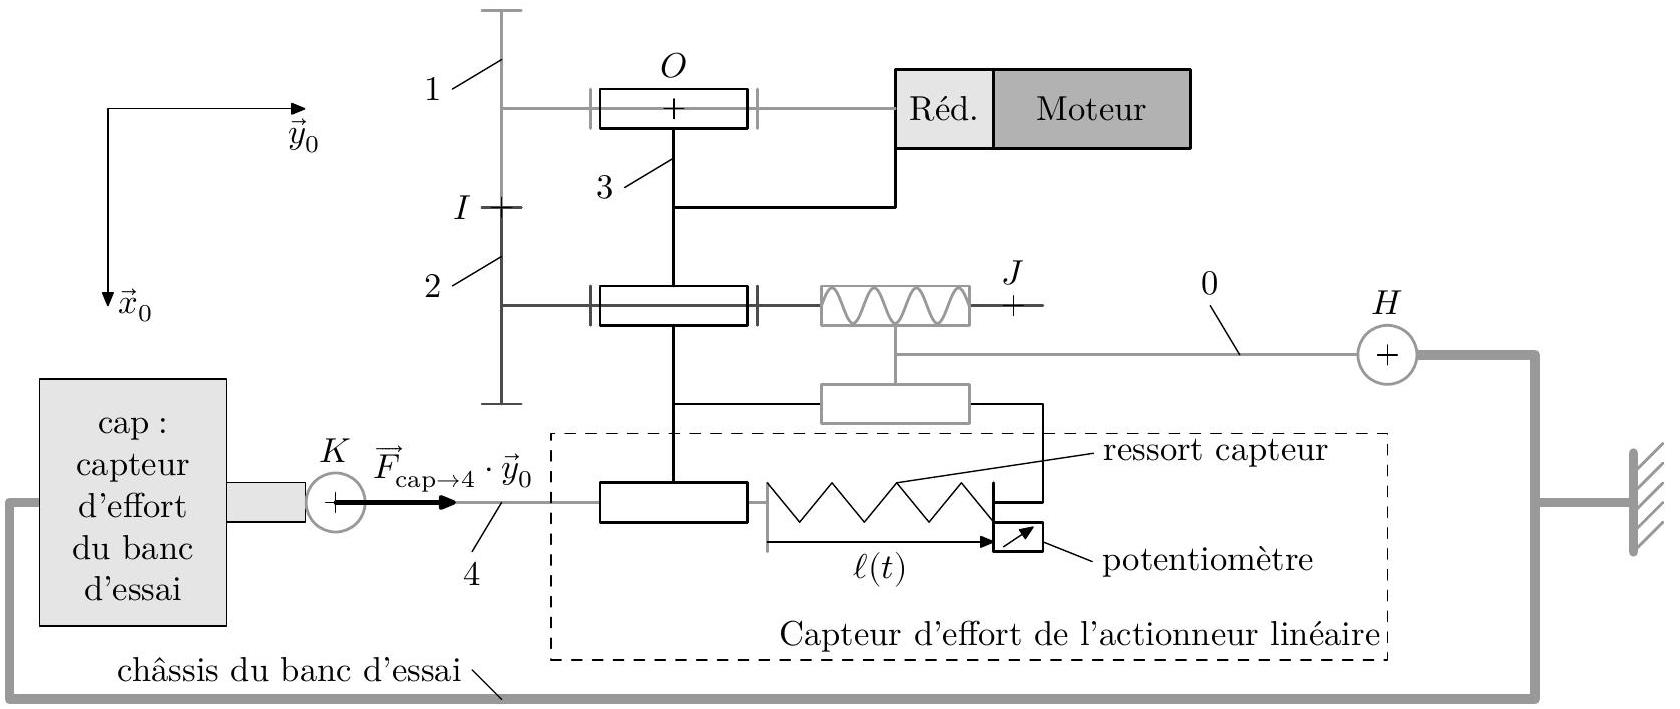
\includegraphics[width=.9\textwidth]{2025_09_16_5f2d7643f7e649c6833dg-07}
\caption{\label{ccs_mp_2023_fig_10}  Modèle d'étude de l'actionneur linéaire sur le banc d'essai}
\end{figure}



On note $\ell(t)$ le déplacement de (3) par rapport à (4).

On a $y(t)=\ell_{0}-\ell(t)$ avec $\ell_{0}$ la longueur à vide du ressort du capteur installé sur le système réel. Le ressort n'est pas préchargé avant le début de l'essai soit $\ell(t=0)=\ell_{0}$.

Le repère $R_{0}\left(H ; \vec{x}_{0}, \vec{y}_{0}, \vec{z}_{0}\right)$ lié au châssis du banc d'essai est supposé galiléen.

Les différentes grandeurs utiles à cette partie sont regroupées dans le tableau \ref{ccs_mp_2023_tab_03}.

\begin{table}[!h]
\begin{center}
\begin{tabular}{lp{8cm}}
\hline
\textbf{Éléments} & \textbf{Caractéristiques et notation} \\
\hline
Corps du vérin 0 & Masse : $m_{0}$ \\
\hline
\multirow[t]{4}{*}{Moteur} & Couple moteur : $C_{3 \rightarrow \text { arbre moteur }}(t)=c_{m}(t)$ \\

 & Moment d'inertie de l'arbre moteur suivant son axe : $I_{m}$ \\

 & Vitesse de rotation de l'arbre moteur : $\omega_{m}(t)=\omega_{m / 3}$ \\

 & Masse négligeable devant les autres masses \\
\hline
\multirow[t]{4}{*}{Réducteur planétaire + pignon 1} & Vitesse de rotation en sortie du réducteur : $\omega_{r}(t)=\omega_{1 / 3}$ \\

 & Rapport de réduction : $\lambda=\frac{\omega_{r}(t)}{\omega_{m}(t)}$ \\

 & Moment d'inertie équivalent reporté sur l'arbre de sortie du réducteur : $I_{r}$ \\

 & Masse négligeable devant les autres masses \\
\hline
\multirow[t]{2}{*}{Transmetteur par engrenage} & Nombre de dents du pignon d'entrée 1: $Z_{1}$ \\

 & Nombre de dents du pignon de sortie 2 : $Z_{2}=Z_{1}$ \\
\hline
\multirow[t]{3}{*}{Vis + pignon 2} & Moment d'inertie suivant l'axe ( $J, \vec{y}_{0}$ ) : $I_{V}$ \\

 & Vis de pas géométrique : pas en $\mathrm{m} \cdot \operatorname{tr}^{-1}$ \\

 & Masse négligeable devant les autres masses \\
\hline
\multirow[t]{2}{*}{Ressort} & Raideur $K_{\text {res }}$ \\

 & Masse négligeable devant les autres masses \\
\hline
Ensemble 3 & Masse $m_{3}$ (les masses du carter moteur et du carter réducteur sont comprises dans la masse $m_{3}$ ) \\
\hline
Tige de vérin 4 & Masse : $m_{4}$ \\
\hline
Rendement & Rendement global de l'actionneur linéaire, supposé constant : $\eta$ \\
\hline
\end{tabular}
%\captionsetup{labelformat=empty}
\caption{\label{ccs_mp_2023_tab_03} Caractéristiques principales de l'actionneur linéaire}
\end{center}
\end{table}

%Q 5. 
\question{\label{ccs_mp_2023_q_05}
En prenant soin de préciser le solide isolé et le théorème utilisé, déterminer l'expression littérale de la résultante $\vec{F}_{\text {cap } \rightarrow 4}$ en projection sur $\vec{y}_{0}$, en fonction de $K_{\text {res }}$ et $y(t)$.}
\ifprof
\begin{corrige}
\end{corrige}
\else
\fi

%Q 6. 
\question{\label{ccs_mp_2023_q_06}
Déterminer le rapport $\frac{\omega_{1 / 3}}{\omega_{2 / 3}}$ en fonction de $Z_{1}$ et $Z_{2}$ et faire l'application numérique. En déduire l'expression de $\vec{V}_{J, 3 / R_{0}}$ en fonction de $\omega_{m}(t)$, pas et $\lambda$.\\
}
\ifprof
\begin{corrige}
\end{corrige}
\else
\fi

On note $\Sigma=\left\{(0)\right.$, arbre moteur, (1), (2), (3), ressort, (4)\} l'ensemble mobile en mouvement par rapport à $R_{0}$.\\

%Q 7. 
\question{\label{ccs_mp_2023_q_07}
Déterminer l'expression des énergies cinétiques $E_{c}\left(\right.$ arbre moteur $\left./ R_{0}\right), E_{c}\left(1 / R_{0}\right), E_{c}\left(2 / R_{0}\right)$ et $E_{c}\left(3 / R_{0}\right)$ en fonction de $\omega_{m}(t)$, pas, $\lambda$, de la masse $m_{3}$ et des inerties.}
\ifprof
\begin{corrige}

\end{corrige}
\else
\fi


%Q 8. \\
\question{\label{ccs_mp_2023_q_08}
Écrire l'expression de l'énergie cinétique $E_{c}\left(\Sigma / R_{0}\right)$ et en déduire l'expression du moment d'inertie équivalent $I_{\text {eq }}$ de l'ensemble mobile $\Sigma$ reporté sur l'arbre moteur en fonction de pas, $\lambda$, de la masse $m_{3}$ et des inerties.}
\ifprof
\begin{corrige}
\end{corrige}
\else
\fi


%Q 9. \\
\question{\label{ccs_mp_2023_q_09}
Établir le bilan des puissances galiléennes des actions extérieures s'exerçant sur $\Sigma$ et montrer qu'elles sont toutes nulles.}
\ifprof
\begin{corrige}
\end{corrige}
\else
\fi


%Q 10. \\
\question{\label{ccs_mp_2023_q_10}
Établir le bilan des puissances des actions intérieures à $\Sigma$ et déterminer leurs expressions littérales en justifiant les résultats.}
\ifprof
\begin{corrige}
\end{corrige}
\else
\fi


%Q 11. 
\question{\label{ccs_mp_2023_q_11}
Par composition des vecteurs vitesse en $K$ entre les solides (4), (3) et (0), déterminer la relation entre $\dot{y}(t), \omega_{m}(t)$, pas et $\lambda$.}
\ifprof
\begin{corrige}
\end{corrige}
\else
\fi


Pour la suite, on définit $K_{\text {trans }}$ tel que $\dot{y}(t)=K_{\text {trans }} \cdot \omega_{m}(t)$.\\

%Q 12. 
\question{\label{ccs_mp_2023_q_12}
En appliquant le théorème de l'énergie cinétique à l'ensemble $\Sigma$ en mouvement par rapport à $R_{0}$, montrer que l'équation de mouvement s'écrit sous la forme 
$
I_{\mathrm{eq}} \frac{\mathrm{~d} \omega_{m}(t)}{\mathrm{d} t}=Q c_{m}(t)-c_{r}(t) \quad \text { avec } \quad c_{r}(t)=T y(t)
$
où l'on précisera les expressions de $Q$ et $T$ en fonction de $\eta, K_{\text {res }}$ et $K_{\text {trans }}$.\\}
\ifprof
\begin{corrige}
\end{corrige}
\else
\fi


%Q 13. \\
\question{\label{ccs_mp_2023_q_13}
Exprimer l'équation différentielle du mouvement liant le déplacement $y(t)$ à l'action mécanique $c_{m}(t)$ en fonction des paramètres de $Q, T$ et $K_{\text {trans }}$. En déduire la valeur numérique du facteur d'amortissement et conclure quant à l'amortissement de la réponse indicielle.}
\ifprof
\begin{corrige}
\end{corrige}
\else
\fi

Cet ensemble d'équations permet de mettre en place un modèle de connaissance de l'actionneur linéaire placé sur le banc d'essai et son analyse justifie la mise en place d'une structure particulière de l'asservissement.

\subsection{Étude de l'effort d'assistance nécessaire au soutien lombaire}%III.B - 
%\section{Objectif}
\begin{obj}
Proposer un modèle de connaissance de l'asservissement en force, le valider par comparaison avec une mesure sur un banc d'essai et vérifier les performances de l'actionneur linéaire sur un banc d'essai. Ce modèle permettra de valider une commande pour le cas spécifique étudié.
\end{obj}


%\section{III.B.1) Mise en place d'un modèle de connaissance}
\subsubsection{Mise en place d'un modèle de connaissance}%III.B.1) 

L'actionneur linéaire placé sur le banc d'essai et sa commande peuvent être modélisés par le schéma-blocs représenté figure \ref{ccs_mp_2023_fig_11}.\\
Notations et hypothèses:

\begin{itemize}
  \item la transformée de Laplace de la fonction $a(t)$ est notée $A(p)$ dans le cas général ;
  \item les conditions de Heaviside sont supposées vérifiées;
  \item $F_{c}(p)$ représente la consigne en force de l'asservissement de force, dans le domaine de Laplace;
  \item $F(p)$ représente la force développée par l'actionneur linéaire, dans le domaine de Laplace.
\end{itemize}

Les équations modélisant le comportement du moteur électrique (moteur à courant continu) muni d'une boucle d'asservissement de l'intensité du courant $i_{m}(t)$, sont :

\begin{itemize}
  \item en supposant le temps de réponse de la boucle de courant négligeable,
\end{itemize}

$$
u_{I}(t)=R i_{m}(t)
$$

\begin{itemize}
  \item par application des théorèmes généraux de la dynamique appliqués à l'ensemble des solides en mouvement,
\end{itemize}

$$
I_{\mathrm{eq}} \frac{\mathrm{~d} \omega_{m}(t)}{\mathrm{d} t}=Q c_{m}(t)-c_{r}(t) \quad \text { avec } \quad c_{r}(t)=T y(t)
$$

\begin{itemize}
  \item loi de couplage électromécanique,
\end{itemize}

$$
c_{m}(t)=k_{c} i_{m}(t)
$$

Avec :

\begin{itemize}
  \item $u_{I}(t)$, la consigne en tension de la boucle d'asservissement de l'intensité du courant $i_{m}(t)$ (en V );
  \item $i_{m}(t)$, l'intensité du courant d'induit absorbé par le moteur à courant continu (en A);
  \item $R$, la résistance d'induit du moteur (en $\Omega$ );
  \item $k_{c}$, la constante de couple (en $\mathrm{N} \cdot \mathrm{m} \cdot \mathrm{A}^{-1}$ );
  \item $I_{\mathrm{eq}}$, le moment d'inertie équivalent des solides en mouvement par rapport au référentiel lié au bâti supposé galiléen, reportée sur l'arbre moteur ( $\mathrm{en} \mathrm{kg} \cdot \mathrm{m}^{2}$ ) ;
  \item $K_{1}$, le gain du modulateur d'énergie.
\end{itemize}

%\begin{figure}[h]
%\begin{center}
%  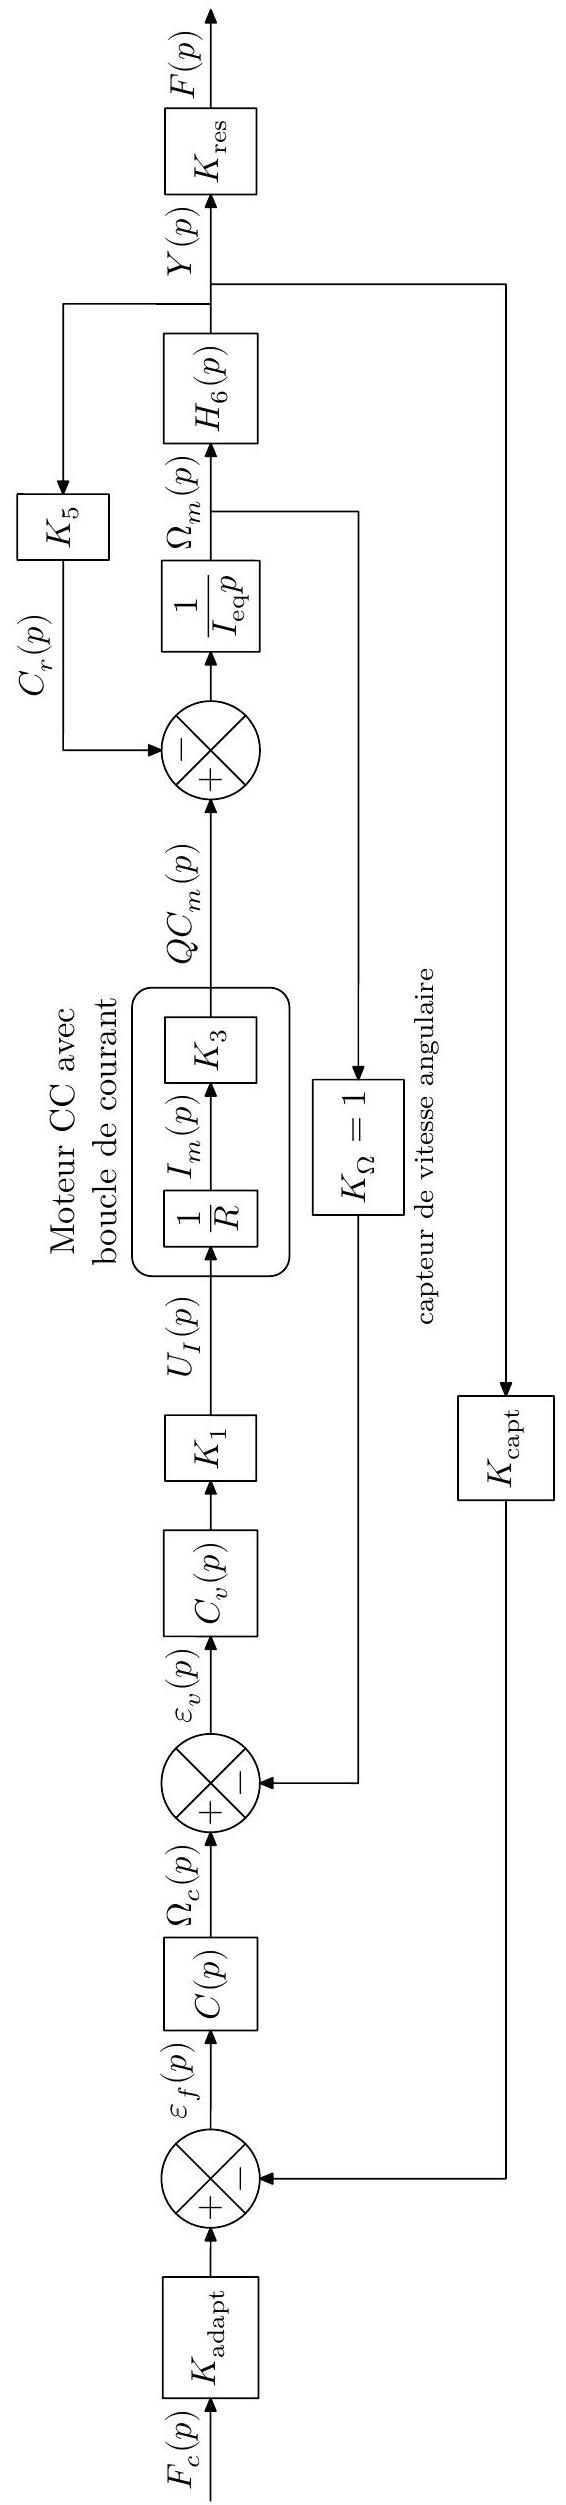
\includegraphics[width=\textwidth]{2025_09_16_5f2d7643f7e649c6833dg-09}
%\captionsetup{labelformat=empty}
%\caption{Figure 11 Schéma-blocs de l'asservissement de force développée par un actionneur linéaire placé sur le banc d'essai}
%\end{center}
%\end{figure}


\begin{figure}[!h]
\centering
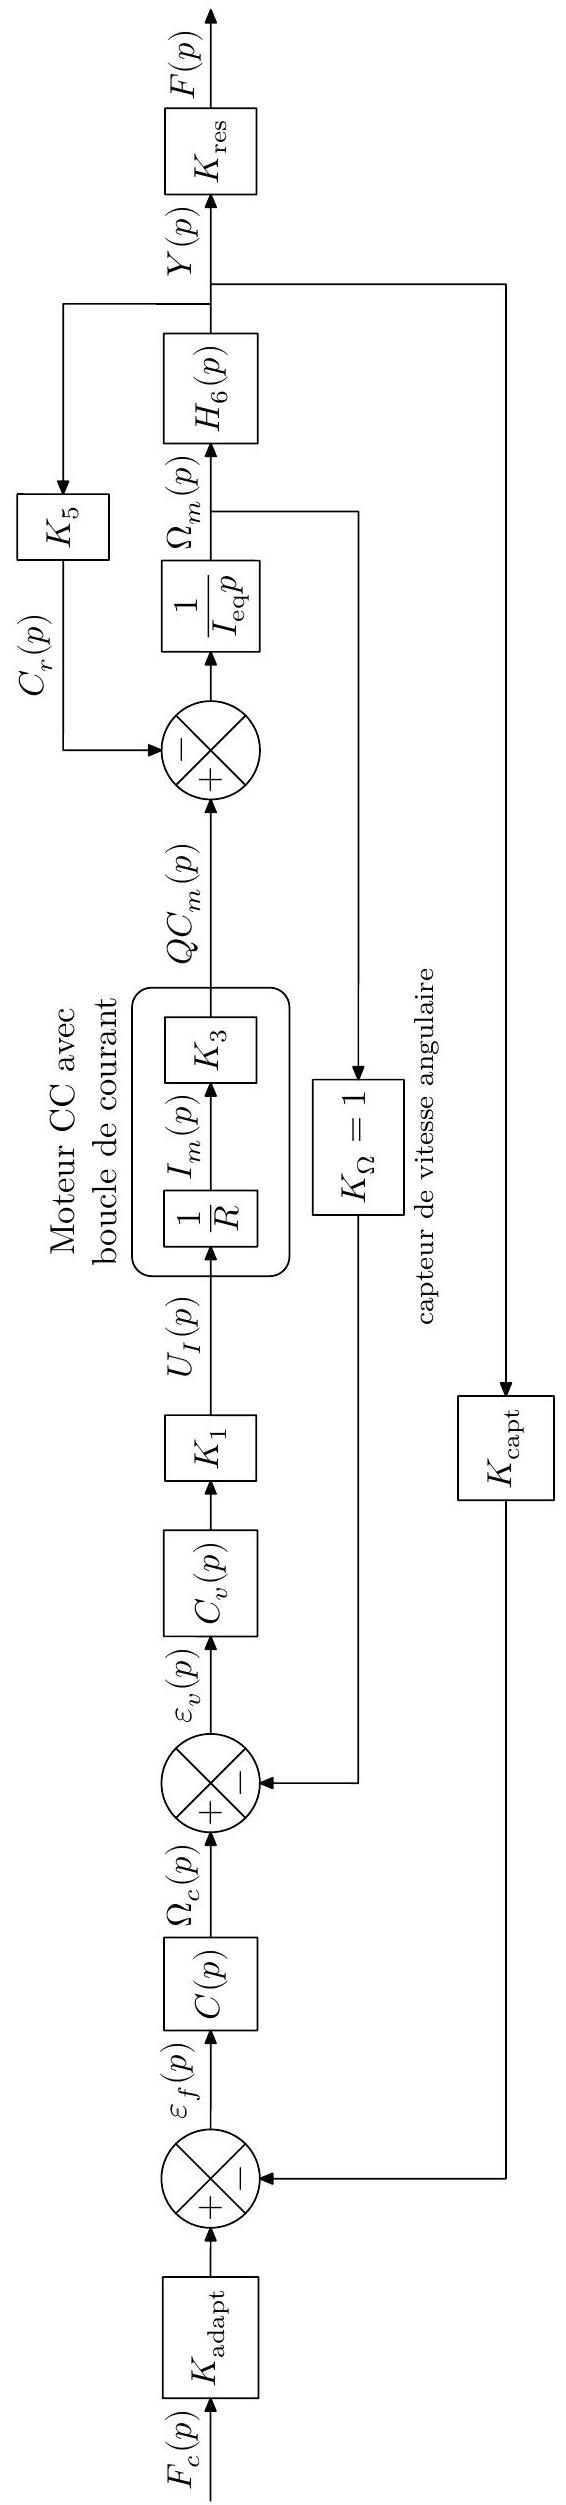
\includegraphics[width=.3\textwidth]{2025_09_16_5f2d7643f7e649c6833dg-09}
\caption{\label{ccs_mp_2023_fig_11}  Schéma-blocs de l'asservissement de force développée par un actionneur linéaire placé sur le banc d'essai}
\end{figure}



%Q 14. \\
\question{\label{ccs_mp_2023_q_14}
Après avoir transformé les équations précédentes dans le domaine de Laplace, exprimer les gains $K_{3}$ et $K_{5}$ en fonction de $Q, k_{c}$ et $T$.}
\ifprof
\begin{corrige}
\end{corrige}
\else
\fi

%Q 15. \\
\question{\label{ccs_mp_2023_q_15}
Exprimer la fonction de transfert $H_{6}(p)$ en fonction de $K_{\text {trans }}$.}
\ifprof
\begin{corrige}
\end{corrige}
\else
\fi


%Q 16. 
\question{\label{ccs_mp_2023_q_16}En supposant le système stable, déterminer l'expression de $K_{\text {adapt }}$ en fonction de $K_{\text {trans }}$ et $K_{\text {res }}$ qui assure que l'écart en régime permanent ( $\varepsilon(t \rightarrow \infty)$ ) soit nul si l'erreur en régime permanent est nulle.}
\ifprof
\begin{corrige}
\end{corrige}
\else
\fi



%
\subsubsection{Réglage de la boucle d'asservissement de la vitesse angulaire du moteur}%III.B.2) 
Le schéma-blocs décrivant la structure de l'asservissement de la vitesse angulaire du moteur est fourni sur la figure \ref{ccs_mp_2023_fig_12}. Cet asservissement doit respecter le cahier des charges fourni dans le tableau \ref{ccs_mp_2023_tab_04}.

%\begin{figure}[h]
%\begin{center}
%  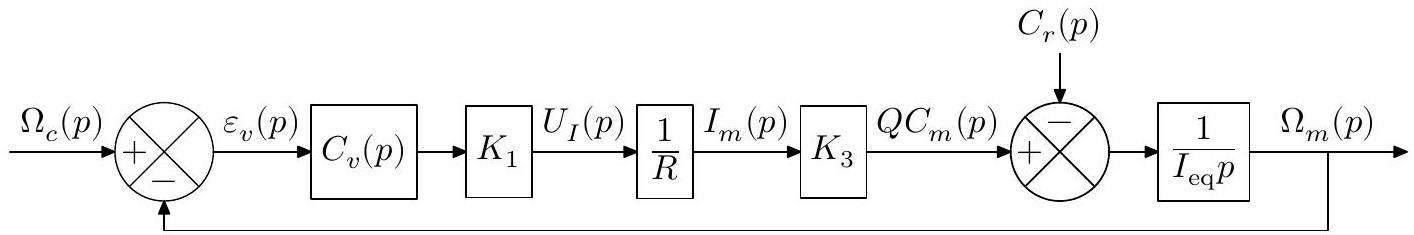
\includegraphics[width=\textwidth]{2025_09_16_5f2d7643f7e649c6833dg-10}
%\captionsetup{labelformat=empty}
%\caption{Figure 12 Schéma-blocs de la boucle d'asservissement de la vitesse angulaire du moteur électrique}
%\end{center}
%\end{figure}


\begin{figure}[!h]
\centering
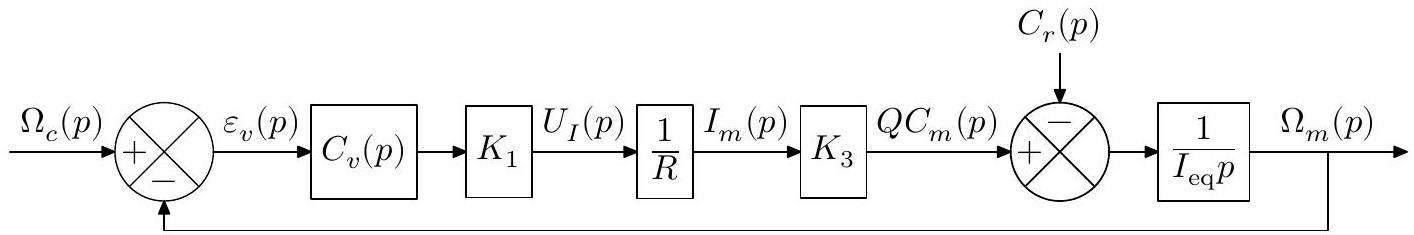
\includegraphics[width=\textwidth]{2025_09_16_5f2d7643f7e649c6833dg-10}
\caption{\label{ccs_mp_2023_fig_12}  Schéma-blocs de la boucle d'asservissement de la vitesse angulaire du moteur électrique}
\end{figure}



\begin{table}[h]
\begin{center}
\begin{tabular}{|l|l|}
\hline
Critère concepteur & Niveau \\
\hline
Marge de phase & $\geqslant 80^{\circ}$ \\
\hline
Erreur en régime permanent pour une perturbation en échelon constante & Nulle \\
\hline
Pulsation de coupure à 0 dB & $\omega_{0 \mathrm{~dB}}=10 \mathrm{rad} \cdot \mathrm{s}^{-1}$ \\
\hline
\end{tabular}
%\captionsetup{labelformat=empty}
\caption{\label{ccs_mp_2023_tab_04}Critères concepteur pour la boucle d'asservissement de la vitesse angulaire}
\end{center}
\end{table}

Le choix d'un correcteur proportionnel intégral est fait afin de diminuer l'influence de la perturbation en couple modélisée par $C_{r}(p)$. La fonction de transfert du correcteur de la boucle d'asservissement en vitesse angulaire est noté $C_{v}(p)$, tel que

$$
C_{v}(p)=K_{i} \frac{1+\tau_{i} p}{\tau_{i} p} .
$$

On note $H_{B O v}(p)=\frac{\Omega_{m}(p)}{\varepsilon_{v}(p)}$ la fonction de transfert en boucle ouverte de l'asservissement de vitesse angulaire du moteur.

%Q 17. 
\question{\label{ccs_mp_2023_q_17}
Déterminer l'expression littérale de la phase de $H_{B O v}(\mathrm{i} \omega)$. En déduire la valeur numérique de $\tau_{i}$ respectant les critères concepteur de la boucle de vitesse.}
\ifprof
\begin{corrige}
\end{corrige}
\else
\fi


Le diagramme de Bode de la boucle ouverte $H_{B O v}(p)$, avec $K_{i}=1$ et $\tau_{i}$ déterminé à la question \ref{ccs_mp_2023_q_17}, est donné sur la figure \ref{ccs_mp_2023_fig_13}.

%\begin{figure}[h]
%\begin{center}
%  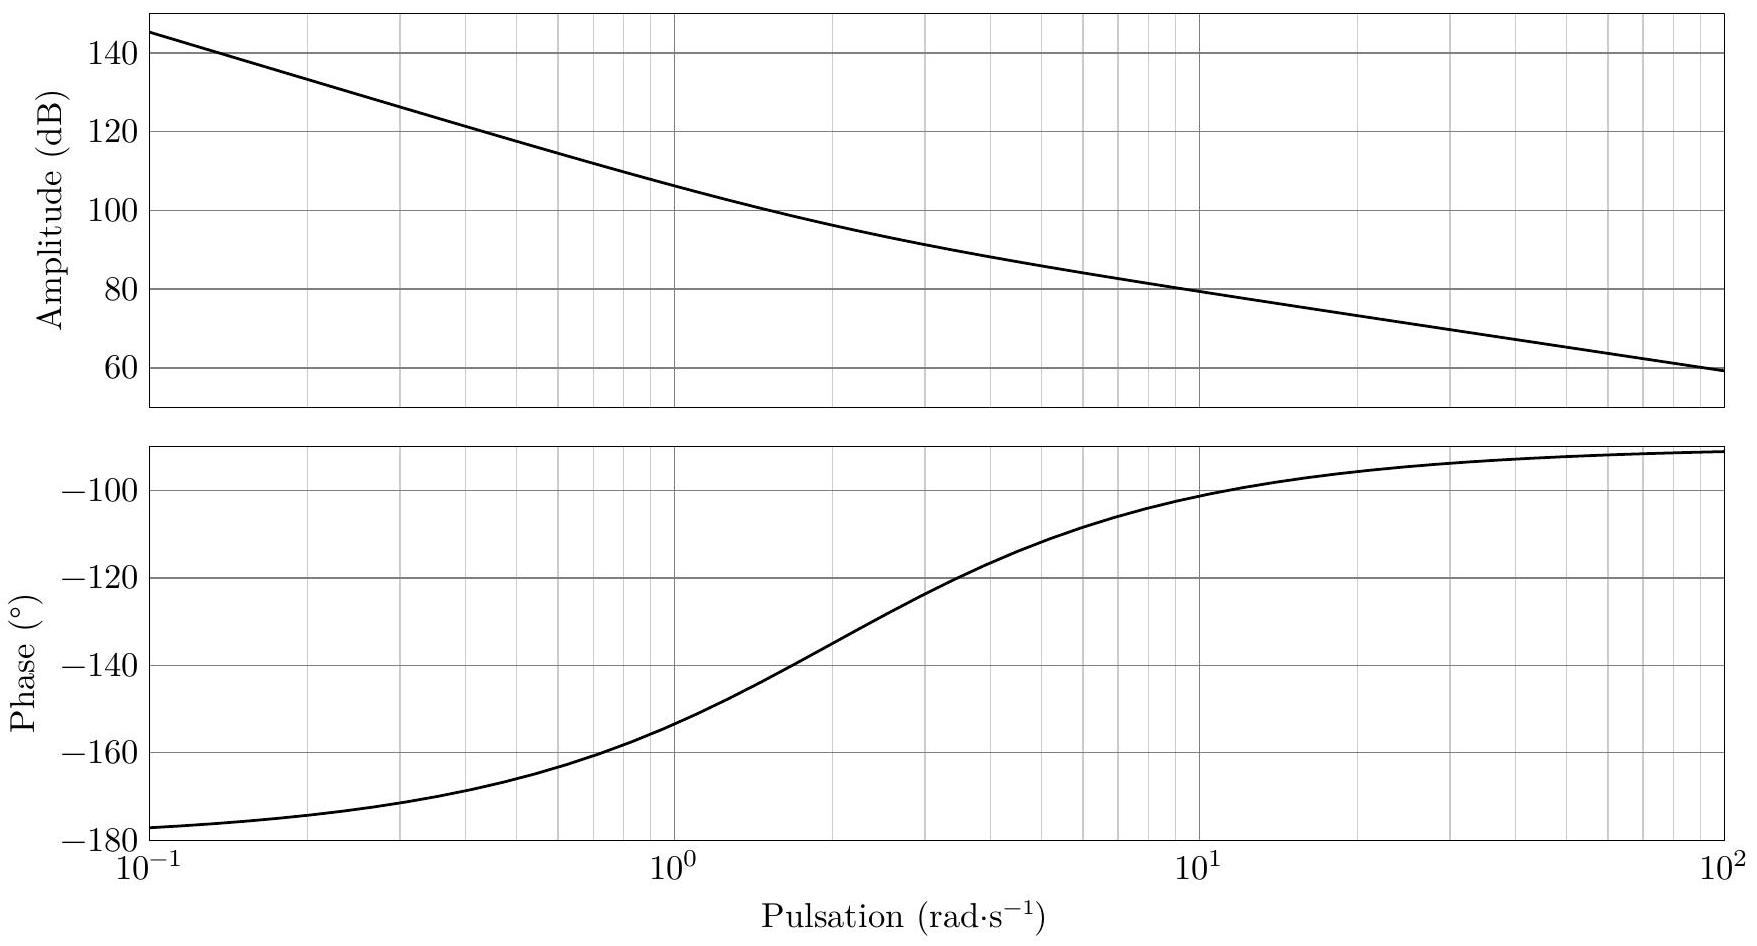
\includegraphics[width=\textwidth]{2025_09_16_5f2d7643f7e649c6833dg-10(1)}
%\captionsetup{labelformat=empty}
%\caption{Figure 13 Diagramme de Bode de \$H\_\{B O v}(p)\$\}\end{center}
%\end{figure}


\begin{figure}[!h]
\centering
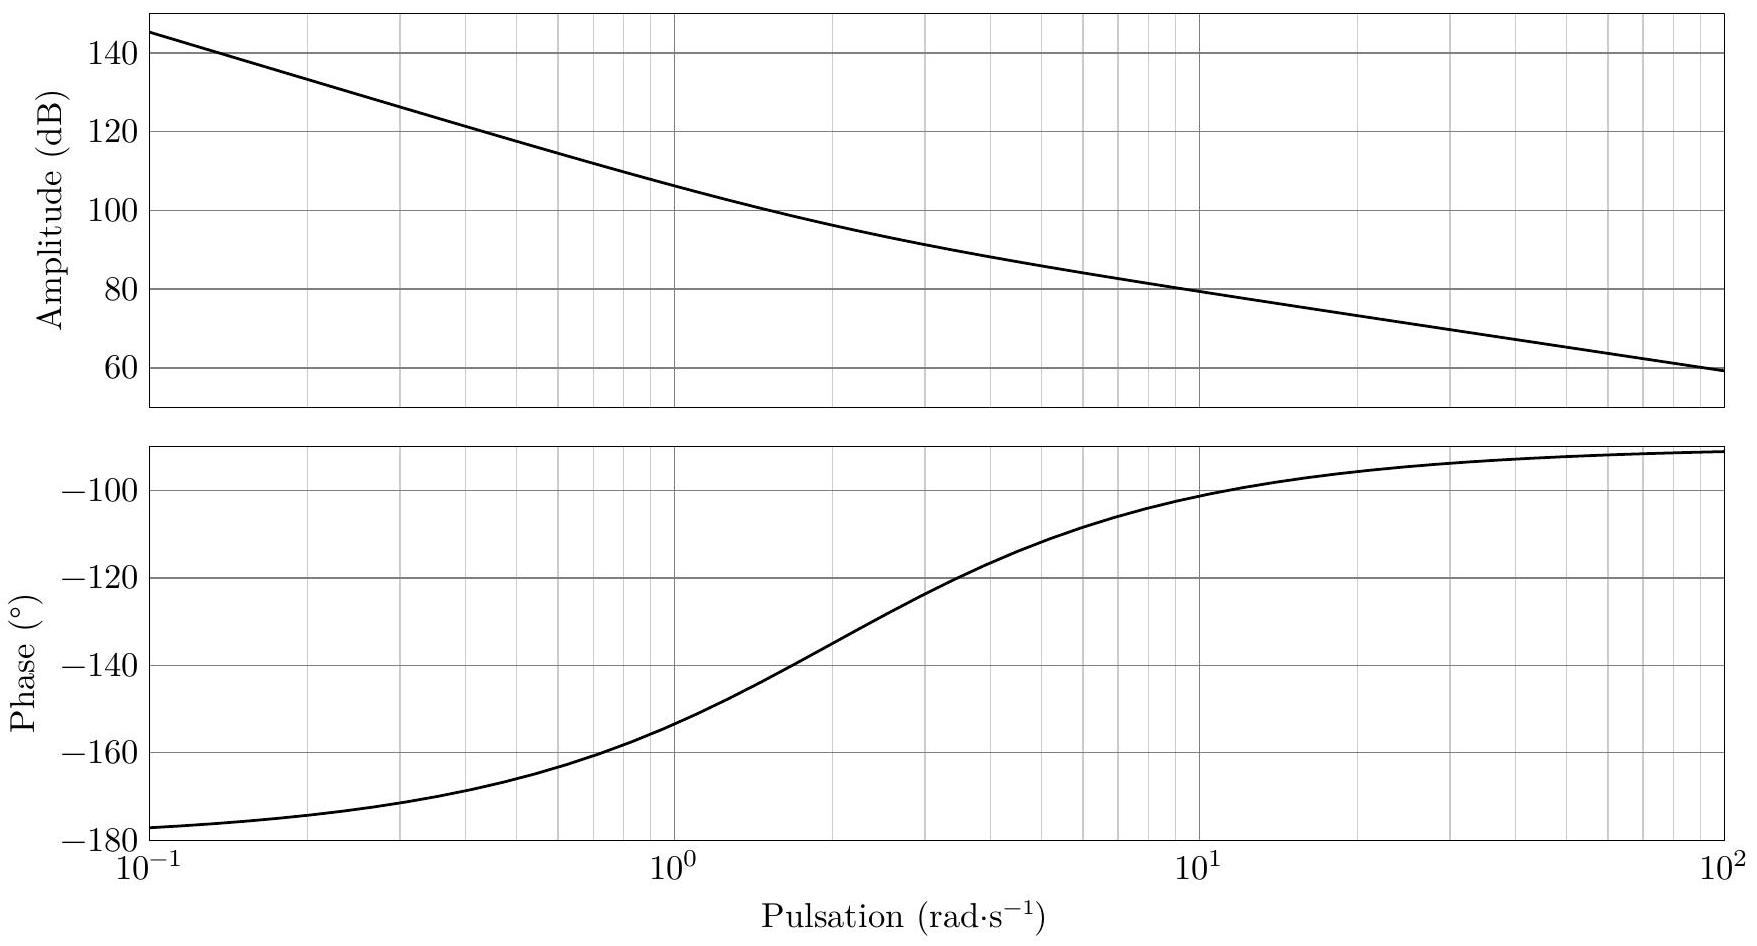
\includegraphics[width=.8\textwidth]{2025_09_16_5f2d7643f7e649c6833dg-10(1)}
\caption{\label{ccs_mp_2023_fig_13}   Diagramme de Bode de \$H\_\{B O v}(p)\$\}
\end{figure}



%Q 18. 
\question{\label{ccs_mp_2023_q_18}
Déterminer la valeur numérique de $K_{i}$ afin que la boucle d'asservissement de vitesse respecte les critères concepteur du tableau \ref{ccs_mp_2023_tab_04}.}
\ifprof
\begin{corrige}
\end{corrige}
\else
\fi



\subsubsection{Simplification du modèle de connaissance}%III.B.3) 
Il est possible de mettre le schéma-blocs de la figure \ref{ccs_mp_2023_fig_11} sous la forme du schéma-blocs de la figure \ref{ccs_mp_2023_fig_14}, afin de faciliter la prévision des performances simulées.

%\begin{figure}[h]
%\begin{center}
%  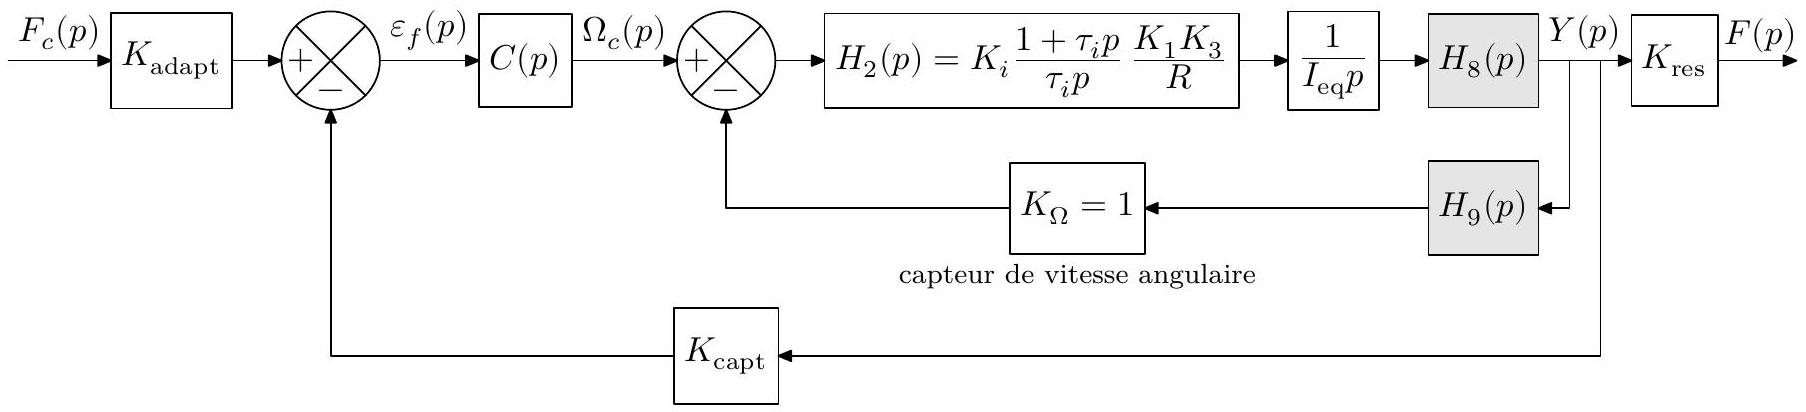
\includegraphics[width=\textwidth]{2025_09_16_5f2d7643f7e649c6833dg-11(1)}
%\captionsetup{labelformat=empty}
%\caption{Figure 14 Schéma-blocs de l'asservissement de la force développée par un actionneur linéaire}
%\end{center}
%\end{figure}


\begin{figure}[!h]
\centering
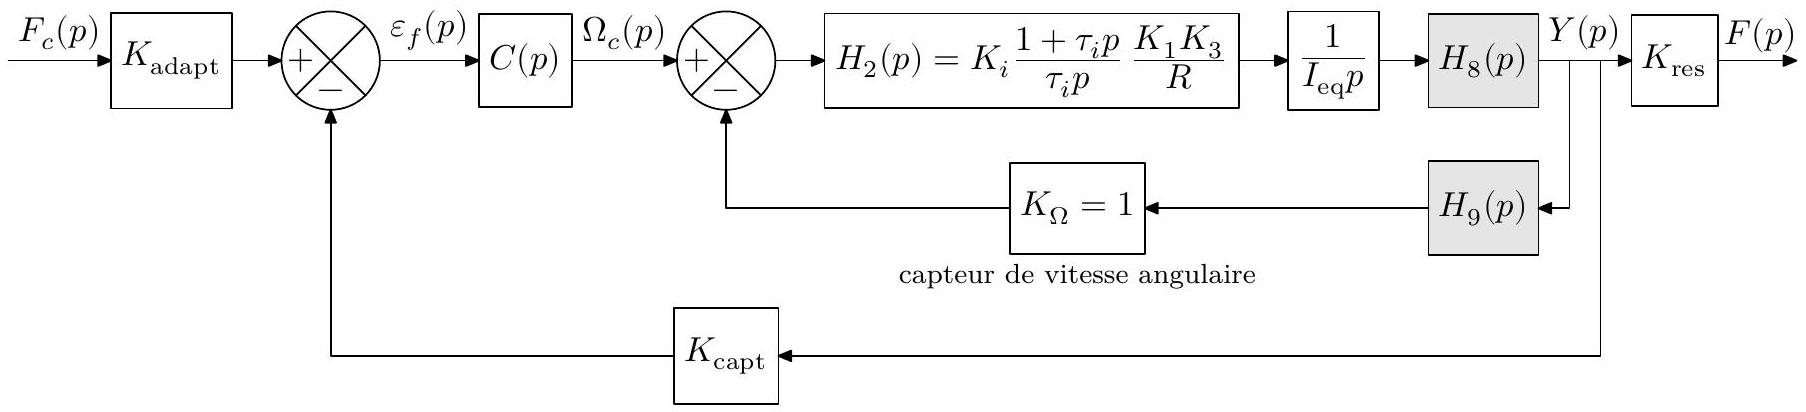
\includegraphics[width=.8\textwidth]{2025_09_16_5f2d7643f7e649c6833dg-11(1)}
\caption{\label{ccs_mp_2023_fig_14} Schéma-blocs de l'asservissement de la force développée par un actionneur linéaire }
\end{figure}



%Q 19. 
\question{\label{ccs_mp_2023_q_19}
Déterminer les fonctions de transfert $H_{8}(p)$ et $H_{9}(p)$ en fonction de $K_{5}, I_{\text {eq }}$ et $H_{6}(p)$. Ne pas remplacer $K_{5}$ et $H_{6}(p)$ par les expressions trouvées précédemment.\\
Pour faciliter l'analyse des performances simulées, le schéma-blocs de la figure \ref{ccs_mp_2023_fig_14} est adapté afin de disposer d'un schéma-blocs à retour unitaire, tel que décrit sur la figure \ref{ccs_mp_2023_fig_15}.}
\ifprof
\begin{corrige}
\end{corrige}
\else
\fi


%\begin{figure}[h]
%\begin{center}
%  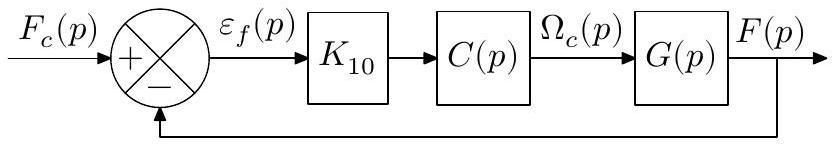
\includegraphics[width=\textwidth]{2025_09_16_5f2d7643f7e649c6833dg-11}
%\captionsetup{labelformat=empty}
%\caption{Figure 15 Schéma-blocs de l'asservissement de la force développée par un actionneur linéaire à retour unitaire}
%\end{center}
%\end{figure}


\begin{figure}[!h]
\centering
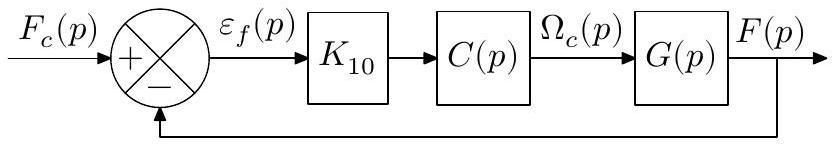
\includegraphics[width=.6\textwidth]{2025_09_16_5f2d7643f7e649c6833dg-11}
\caption{\label{ccs_mp_2023_fig_15} Schéma-blocs de l'asservissement de la force développée par un actionneur linéaire à retour unitaire}
\end{figure}

%Q 20. \\
\question{\label{ccs_mp_2023_q_20}
Déterminer l'expression du gain $K_{10}$ en fonction de $K_{\text {capt }}$ et de $K_{\text {res }}$.}
\ifprof
\begin{corrige}
\end{corrige}
\else
\fi


%Q 21. 

\question{\label{ccs_mp_2023_q_21}
Déterminer la fonction de transfert $G(p)$ en fonction de $H_{2}(p), I_{\text {eq }}, H_{8}(p), H_{9}(p)$ et $K_{\text {res }}$. Ne pas remplacer $H_{2}(p), H_{8}(p)$ et $H_{9}(p)$ par les expressions trouvées précédemment.\\}
\ifprof
\begin{corrige}
\end{corrige}
\else
\fi


Pour la suite, on donne la fonction de transfert $G(p)$, obtenue avec les valeurs de réglage correctes déterminées aux questions \ref{ccs_mp_2023_q_17} et \ref{ccs_mp_2023_q_18},
$$
G(p)=\frac{F(p)}{\Omega_{c}(p)}=\frac{1+\tau_{i} p}{p} \frac{1,2 \times 10^{-5}}{2 \times 10^{-4}+9,7 \times 10^{-5} p+5,3 \times 10^{-6} p^{2}} .
$$

\subsubsection{Analyse des performances de l'asservissement en force développée par un actionneur linéaire}%III.B.4) 
Il est proposé dans cette section d'analyser les performances simulées de l'asservissement en force dont un extrait du cahier des charges est présenté dans le tableau \ref{ccs_mp_2023_tab_05}.

\begin{table}[h]
\begin{center}
\begin{tabular}{|l|l|l|l|}
\hline
Id & Exigence & Critère & Niveau \\
\hline
\multirow[t]{3}{*}{Id1.1} & \multirow[t]{3}{*}{Stabilité} & Marge de phase & $\geqslant 60^{\circ}$ \\
\hline
 &  & Marge de gain & $>20 \mathrm{~dB}$ \\
\hline
 &  & Dépassement maximal & < 2,5\% \\
\hline
Id1.2 & Précision & Erreur en régime permanent pour une entrée en échelon & < 1\% \\
\hline
\multirow[t]{2}{*}{Id1.3} & \multirow[t]{2}{*}{Rapidité} & Temps de réponse à $5 \%$ pour une consigne en échelon de force de 40 N & $\operatorname{tr}_{5 \%}<1 \mathrm{~s}$ \\
\hline
 &  & Vitesse maximale de montée de la force de traction & $100 \mathrm{~N} \cdot \mathrm{~s}^{-1}$ \\
\hline
\end{tabular}
%\captionsetup{labelformat=empty}
\caption{\label{ccs_mp_2023_tab_05}Extrait du cahier des charges fonctionnel de l'actionneur linéaire sur le banc d'essai}
\end{center}
\end{table}

On note $H_{B O f}(p)=\frac{F(p)}{\varepsilon_{f}(p)}$ la fonction de transfert en boucle ouverte de l'asservissement en force développé par un actionneur linéaire. Dans un premier temps, le choix d'un correcteur proportionnel $C(p)=K_{\text {cor }}$ est réalisé. Le diagramme de Bode de la fonction de transfert $H_{B O f}(p)=\frac{F(p)}{\varepsilon_{f}(p)}=K_{\text {cor }} K_{10} G(p)$, avec $K_{\text {cor }}=1$ et la valeur de $\tau_{i}$ déterminée à la question \ref{ccs_mp_2023_q_17}, est donné sur la figure \ref{ccs_mp_2023_fig_16} .

%\begin{figure}[h]
%\begin{center}
%  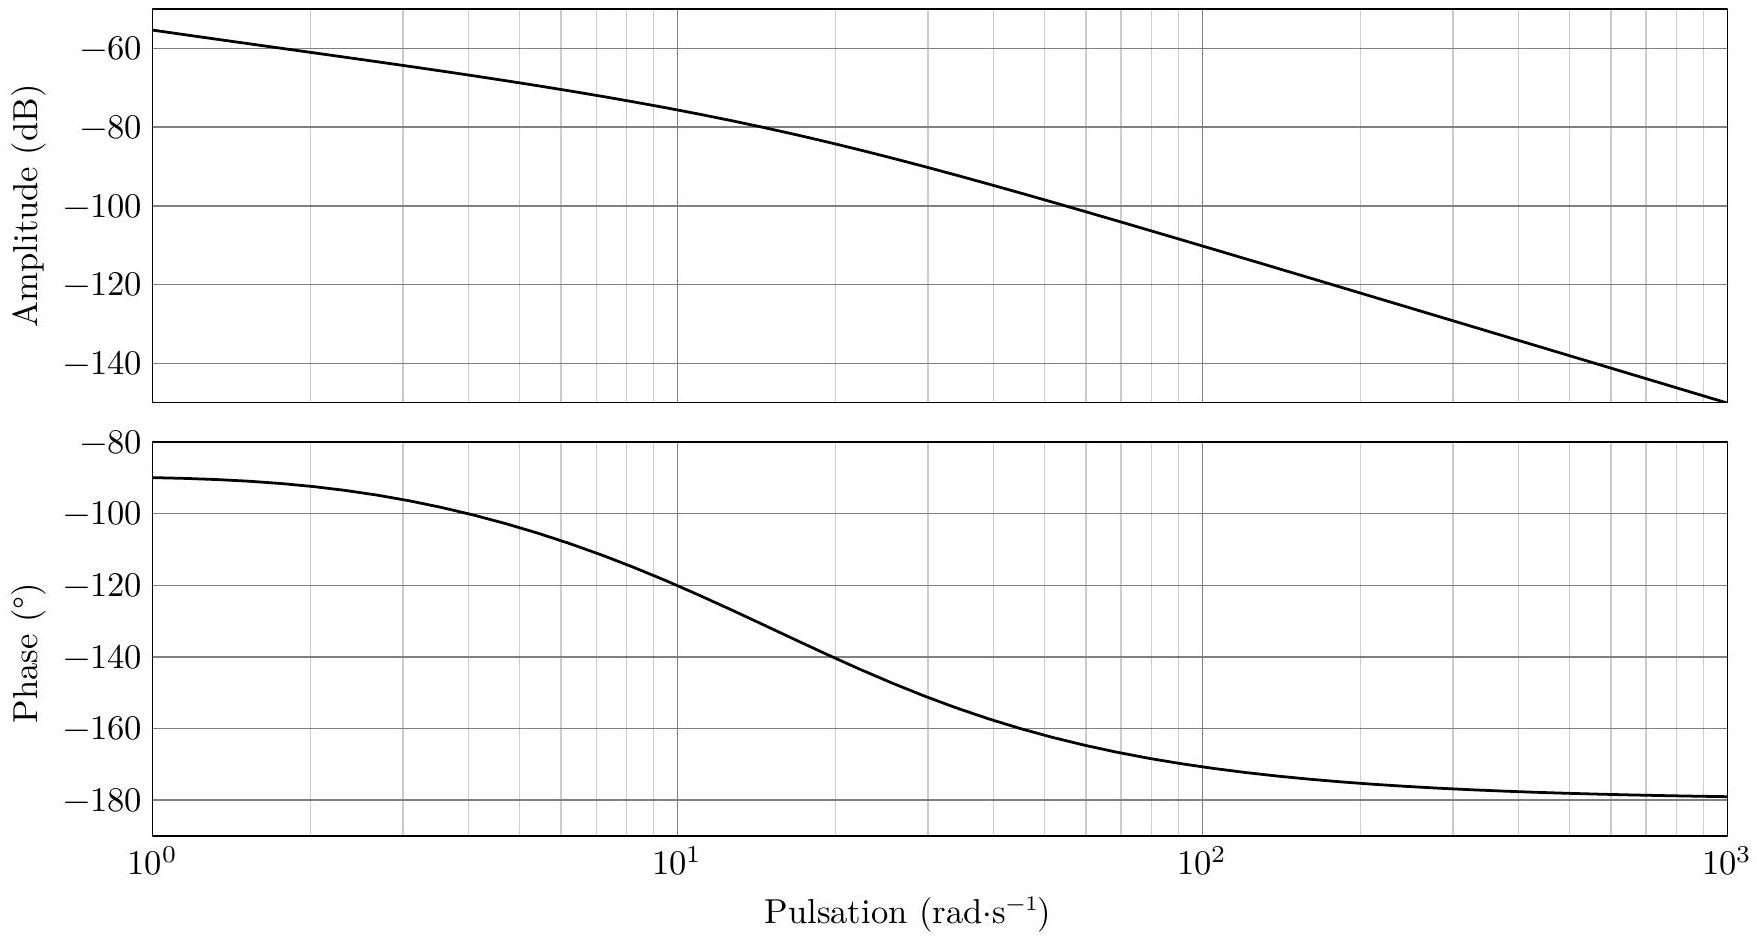
\includegraphics[width=\textwidth]{2025_09_16_5f2d7643f7e649c6833dg-12(1)}
%\captionsetup{labelformat=empty}
%\caption{Figure 16 Diagramme de Bode de \$H\_\{B O f}(p)\$\}
%\end{center}
%\end{figure}


\begin{figure}[!h]
\centering
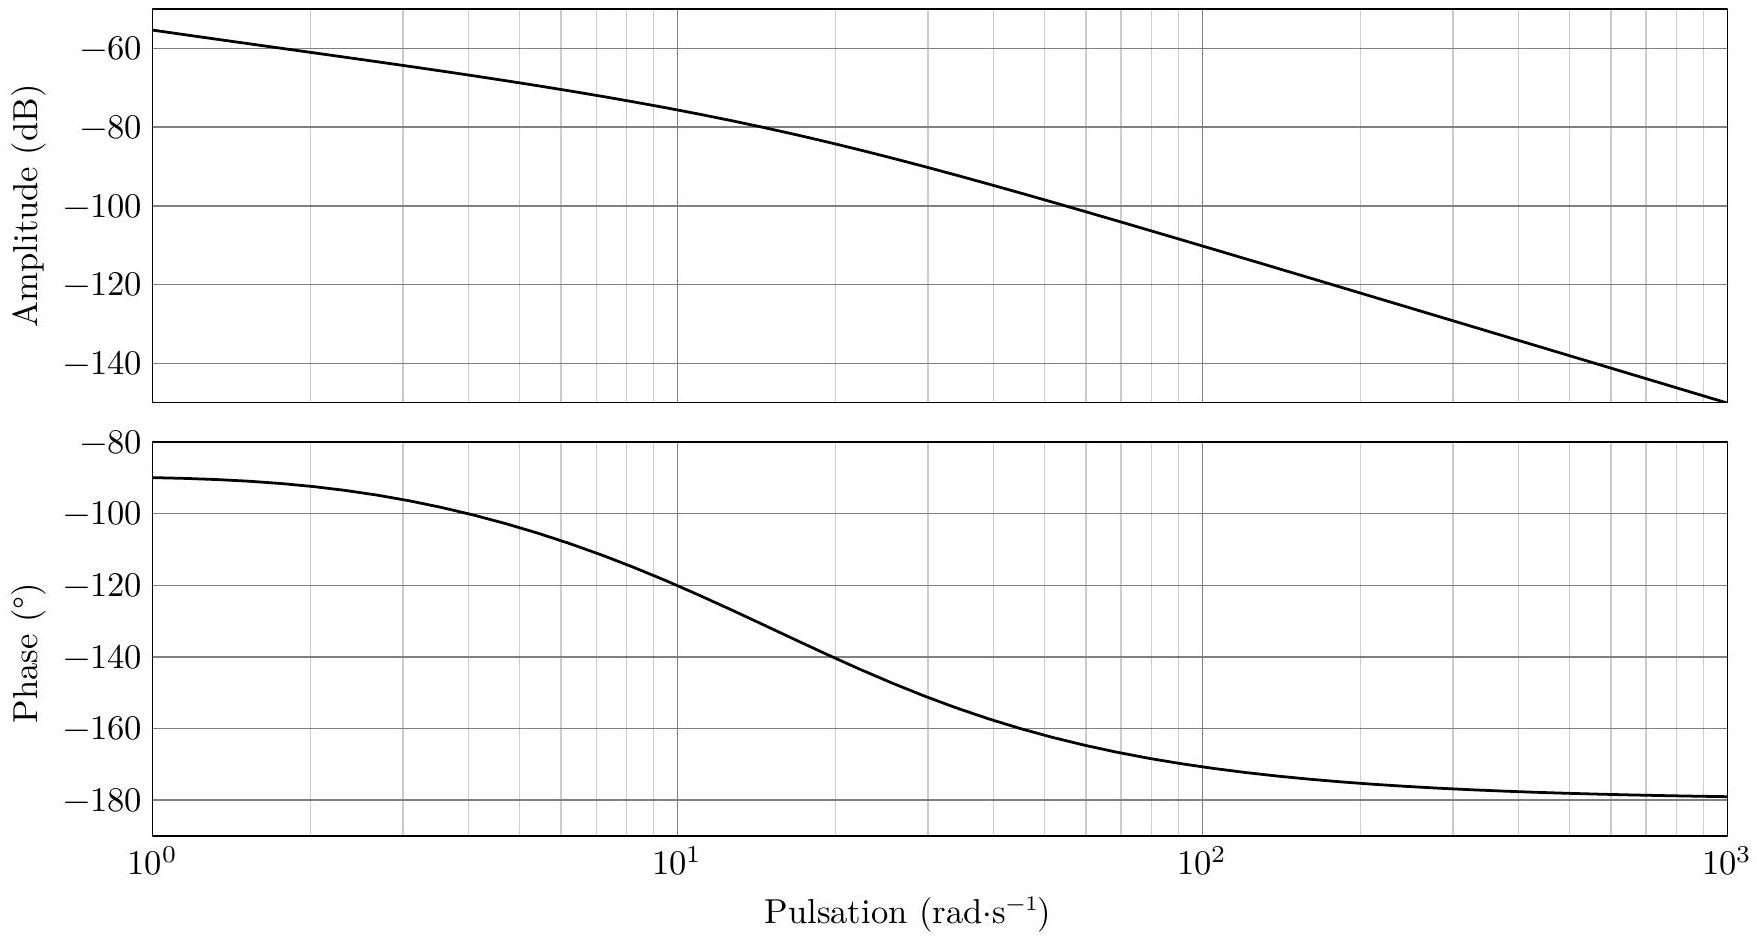
\includegraphics[width=\textwidth]{2025_09_16_5f2d7643f7e649c6833dg-12(1)}
\caption{\label{ccs_mp_2023_fig_16}  Diagramme de Bode de $\indice{H}{BO f}(p)$}
\end{figure}


%Q 22. \\
Les courbes sur la figure \ref{ccs_mp_2023_fig_17} représentent les réponses temporelles du modèle de connaissance de la figure \ref{ccs_mp_2023_fig_11}, avec les correcteurs $C_{v}(p)$ et $C(p)$ correctement réglés, et de l'expérimentation sur le banc d'essai pour une consigne en échelon de force de 40 N .
\question{\label{ccs_mp_2023_q_22}
Déterminer la valeur numérique limite de $K_{\text {cor }}$ afin que la boucle d'asservissement de force respecte les critères de marge de phase et de gain du tableau 5 .}
\ifprof
\begin{corrige}
\end{corrige}
\else
\fi


%\begin{figure}[h]
%\begin{center}
%  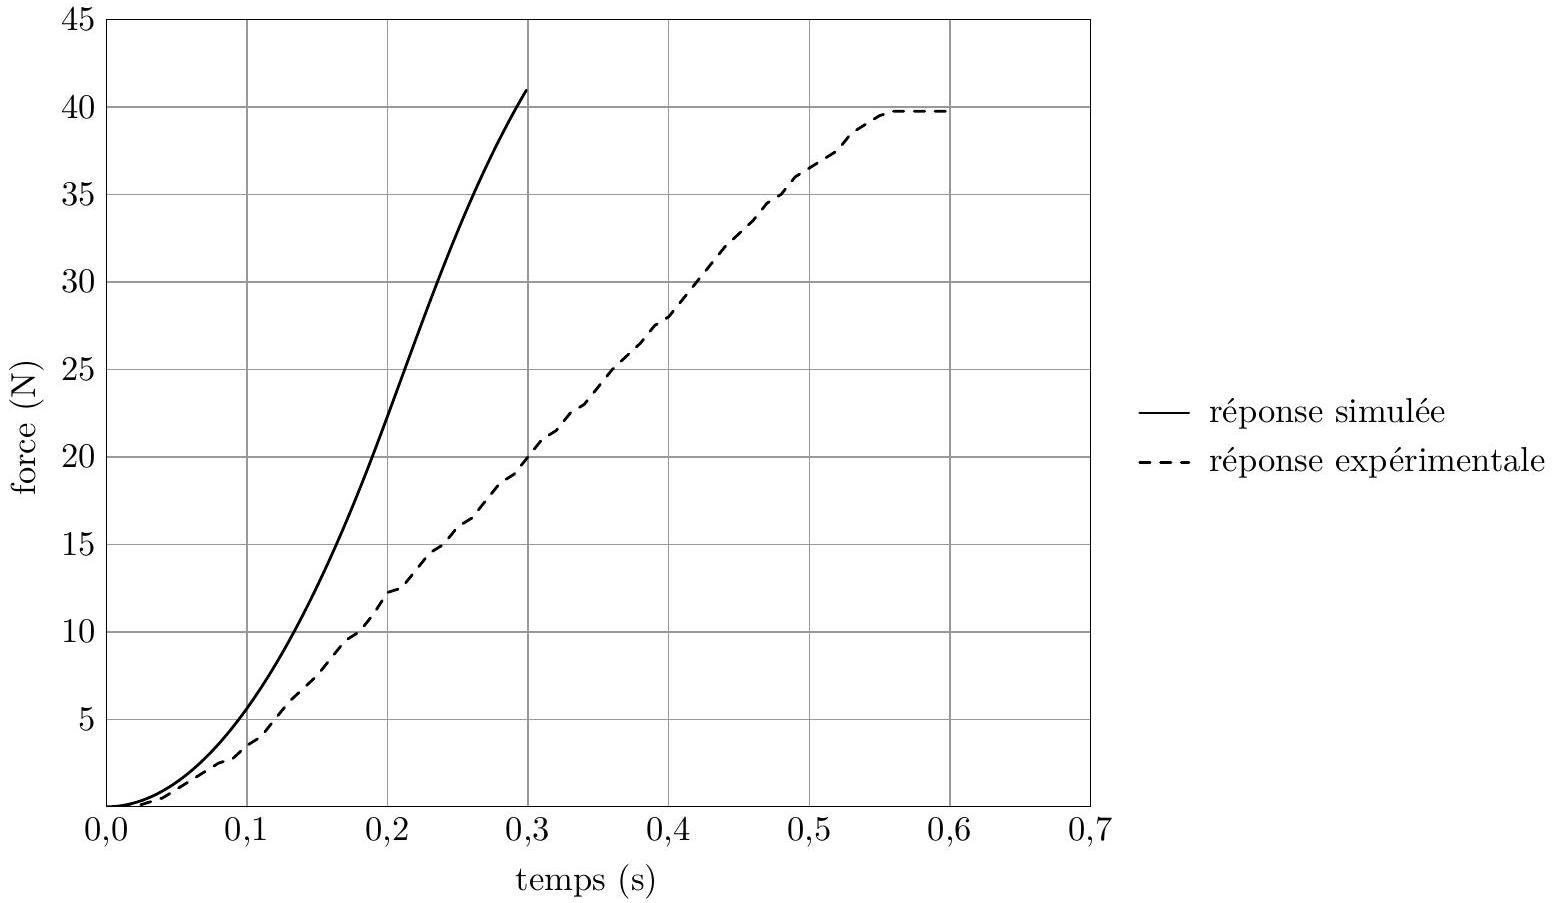
\includegraphics[width=\textwidth]{2025_09_16_5f2d7643f7e649c6833dg-12}
%\captionsetup{labelformat=empty}
%\caption{Figure 17 Réponses temporelles du modèle et expérimentale, pour une consigne en échelon de force de 40 N}
%\end{center}
%\end{figure}


\begin{figure}[!h]
\centering
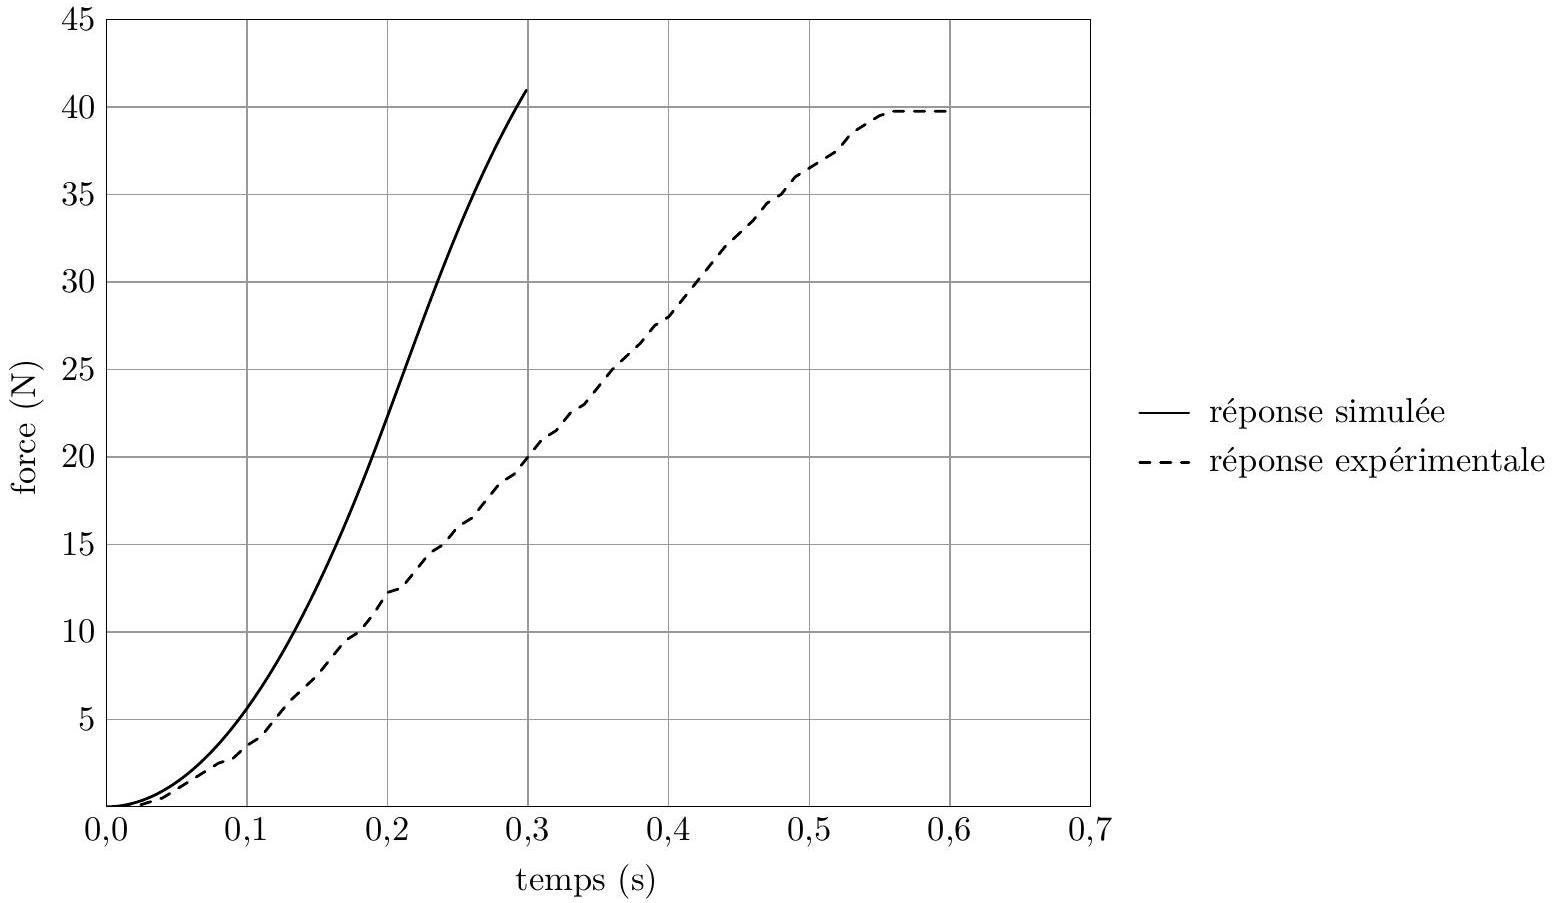
\includegraphics[width=\textwidth]{2025_09_16_5f2d7643f7e649c6833dg-12}
\caption{\label{ccs_mp_2023_fig_17} Réponses temporelles du modèle et expérimentale, pour une consigne en échelon de force de 40 N}
\end{figure}




%Q 23. 
\question{\label{ccs_mp_2023_q_23}
Quel critère du tableau des exigences (tableau \ref{ccs_mp_2023_tab_05}) n'est pas pris en compte dans le modèle de connaissance? D'après la courbe expérimentale, ce critère est-il respecté par le système réel ?}
\ifprof
\begin{corrige}
\end{corrige}
\else
\fi



\subsubsection{ Amélioration du modèle. Mise en place d'une limitation en vitesse angulaire}%III.B.5)
Pour améliorer le modèle de connaissance et le valider, la comparaison entre la réponse simulée issue du modèle de connaissance amélioré et la réponse expérimentale sera traitée par résolution numérique informatique. Le langage de programmation utilisé est Python.

%\begin{figure}[h]
%\begin{center}
%  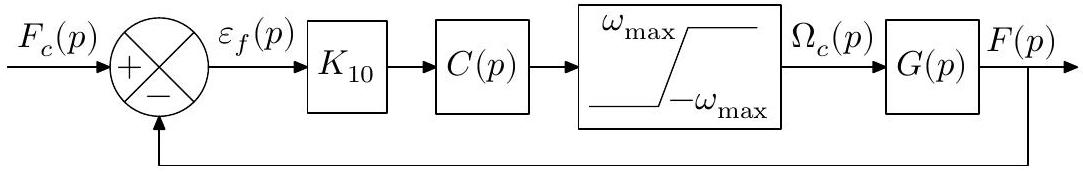
\includegraphics[width=\textwidth]{2025_09_16_5f2d7643f7e649c6833dg-13}
%\captionsetup{labelformat=empty}
%\caption{Figure 18 Schéma-blocs de l'asservissement de force développée par l'actionneur linéaire avec limitation de la vitesse angulaire}
%\end{center}
%\end{figure}


\begin{figure}[!h]
\centering
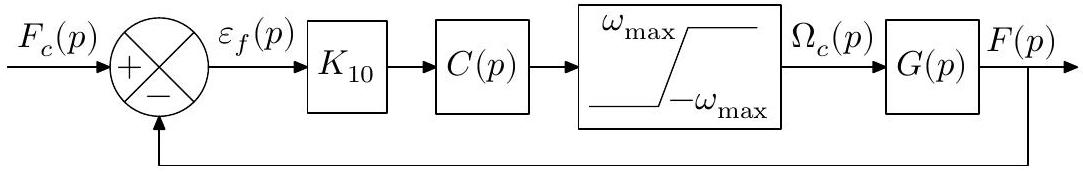
\includegraphics[width=.7\textwidth]{2025_09_16_5f2d7643f7e649c6833dg-13}
\caption{\label{ccs_mp_2023_fig_18}  Schéma-blocs de l'asservissement de force développée par l'actionneur linéaire avec limitation de la vitesse angulaire}
\end{figure}



\textbf{Notations et hypothèses:}

\begin{itemize}
  \item $f(t)$ est la grandeur de sortie de l'asservissement en force, de variable de Laplace $F(p)$;
  \item $f_{c}(t)$ est la grandeur de consigne de l'asservissement en force, de variable de Laplace $F_{c}(p)$;
  \item $\omega_{c}(t)$ est la commande de vitesse angulaire du moteur, de variable de Laplace $\Omega_{c}(p)$;
  \item la dérivée première temporelle d'une fonction $h(t)$ est notée $\dot{h}(t)$ et sa dérivée seconde $\ddot{h}(t)$;
  \item les conditions de Heaviside sont supposées vérifiées, soient $f(t=0)=0$ et $\dot{f}(t=0)=0$.\\
a) Cadre général de la résolution numérique d'un problème de Cauchy
\end{itemize}

Pour déterminer numériquement la solution $E(t)$ d'une équation différentielle, il faut préalablement la mettre sous la forme d'un problème de Cauchy :

$$
\dot{E}(t)=F_{\text {Cauchy }}(E(t), t) \quad \text { avec } \quad E(t=0)=E_{0} .
$$

$E(t)$ est appelé vecteur d'états à l'instant $t, \dot{E}(t)$ représente le vecteur composé des dérivées premières des états par rapport au temps $t, F_{\text {Cauchy }}$ la fonction de Cauchy et $E_{0}$ le vecteur d'états des conditions initiales.\\
Le problème étant décrit sous la forme de Cauchy, la résolution numérique peut être menée par un schéma numérique du type Euler explicite ou en utilisant la fonction odeint de la bibliothèque scipy.\\
b) Problème de Cauchy lié à l'équation différentielle associée à $G(p)$

Compte-tenu du correcteur $C_{v}(p)$ de la boucle d'asservissement de la vitesse angulaire du moteur électrique réglé aux questions \ref{ccs_mp_2023_q_17} et \ref{ccs_mp_2023_q_18}, il est possible de simplifier la fonction de transfert $G(p)$. L'équation différentielle associée à $G(p)$ simplifiée s'écrit

$$
\ddot{f}(t)+18 \dot{f}(t)=1,18 \omega_{c}(t) .
$$

Dans le cadre de la résolution de l'équation différentielle globale liée à l'asservissement de force développée par un actionneur linéaire (figure \ref{ccs_mp_2023_fig_18}), la vitesse angulaire de consigne $\omega_{c}(t)$ est une fonction du temps inconnue à ce stade.\\
Le vecteur d'états associé à l'étude de $G(p)$ retenu est $E(t)=\binom{f(t)}{\dot{f}(t)}$, ainsi $\dot{E}(t)=\binom{\dot{f}(t)}{\ddot{f}(t)}=G\left(E(t), \omega_{c}(t), t\right)$.\\
%Q 24. \\
\question{\label{ccs_mp_2023_q_24}
Déterminer la fonction $G\left(E(t), \omega_{c}(t), t\right)$, associée à $G(p)$.}
\ifprof
\begin{corrige}
\end{corrige}
\else
\fi


%Q 25. 
\question{\label{ccs_mp_2023_q_25}
Écrire en langage Python la fonction $\mathrm{G}(\mathrm{E}, \mathrm{wc}, \mathrm{t})$ qui implémente la fonction $G\left(E(t), \omega_{c}(t), t\right)$. Cette fonction renvoie une liste de deux nombres à virgule flottante et prend en paramètres}
\begin{itemize}
  \item E, une liste de deux nombres représentant le vecteur d'états ;
  \item wc, un nombre représentant la consigne de vitesse angulaire du moteur ;
  \item t, un nombre représentant le temps.\\
c) Problème de Cauchy lié au schéma-blocs de la figure \ref{ccs_mp_2023_fig_18} sans la limitation en vitesse angulaire
\end{itemize}
\ifprof
\begin{corrige}
\end{corrige}
\else
\fi



Le correcteur de la boucle d'asservissement de la force développée par un actionneur linéaire est un correcteur proportionnel tel que $C(p)=K_{\text {cor }}$. Ainsi, en l'absence de limitation, la grandeur $\omega_{c}(t)$ est telle que

$$
\omega_{c}(t)=K_{\operatorname{cor}} K_{10} \varepsilon_{f}(t)=K_{\operatorname{cor}} K_{10}\left(f_{c}(t)-f(t)\right) .
$$

Il reste à exprimer la fonction de Cauchy pour la boucle fermée de l'asservissement de force

$$
\dot{E}(t)=\binom{\dot{f}(t)}{\ddot{f}(t)}=F B F s l(E(t), t) .
$$

On considère dès à présent que la consigne de force $f_{c}(t)$ est un échelon d'amplitude $F_{\text {cons }}$, prise égale à 40 N .\\
Q 26. Recopier et compléter le programme Python de la figure \ref{ccs_mp_2023_fig_19} implémentant la fonction FBFsl qui renvoie une liste de deux nombres et prend en paramètres
\question{\label{ccs_mp_2023_q_}
}
\ifprof
\begin{corrige}
\end{corrige}
\else
\fi



\begin{itemize}
  \item E, une liste de deux nombres représentant le vecteur d'états ;
  \item t, un nombre représentant le temps.
\end{itemize}



\begin{figure}[!h]
\begin{lstlisting}
def FBFsl(E, t):
    Fcons = 40 # échelon de consigne de 40 N
    K10 = 0.0277 # adaptation
    Kcor = 5400 # gain du correcteur proportionnel
    wc = à compléter
    # Compléter en terminant la fonction.
\end{lstlisting}
\caption{\label{ccs_mp_2023_fig_19}  Programme de calcul de la fonction \lstinline{FBFsl}, à compléter}
\end{figure}


d) Problème de Cauchy lié au schéma-blocs de la figure \ref{ccs_mp_2023_fig_18} avec la limitation en vitesse angulaire

La consigne de vitesse angulaire du moteur électrique doit être limitée, conformément au schéma-blocs de la figure \ref{ccs_mp_2023_fig_18}.\\


%Q 27. 
\question{\label{ccs_mp_2023_q_27}
Recopier et compléter le programme Python de la figure \ref{ccs_mp_2023_fig_20} implémentant la fonction FBFal qui renvoie une liste de deux nombres et prend en compte la limitation de la consigne de vitesse angulaire du moteur.}
\ifprof
\begin{corrige}
\end{corrige}
\else
\fi




\begin{figure}[!h]
\begin{lstlisting}
def FBFal(E, t):
    Fcons = 40 # échelon de consigne de 40 N
    K10 = 0.0277 # adaptation
    Kcor = 5400 # gain du correcteur proportionnel
    wcmax = 1250 # limitation en vitesse angulaire dans l'intervalle [-wcmac, wcmax]
    # Compléter avec le calcul de wc et terminer la fonction.
\end{lstlisting}

\caption{\label{ccs_mp_2023_fig_20}  Programme de calcul de la fonction \lstinline{FBFal}, à compléter}
\end{figure}


%Figure 20 
e) Résolution du problème de Cauchy associé au modèle avec limitation en vitesse angulaire

La figure 21 présente la réponse temporelle du modèle de connaissance du système avec correction proportionnelle et limitation pour une consigne de force en échelon d'amplitude $F_{\text {cons }}=40 \mathrm{~N}$.

%\begin{figure}[h]
%\begin{center}
%  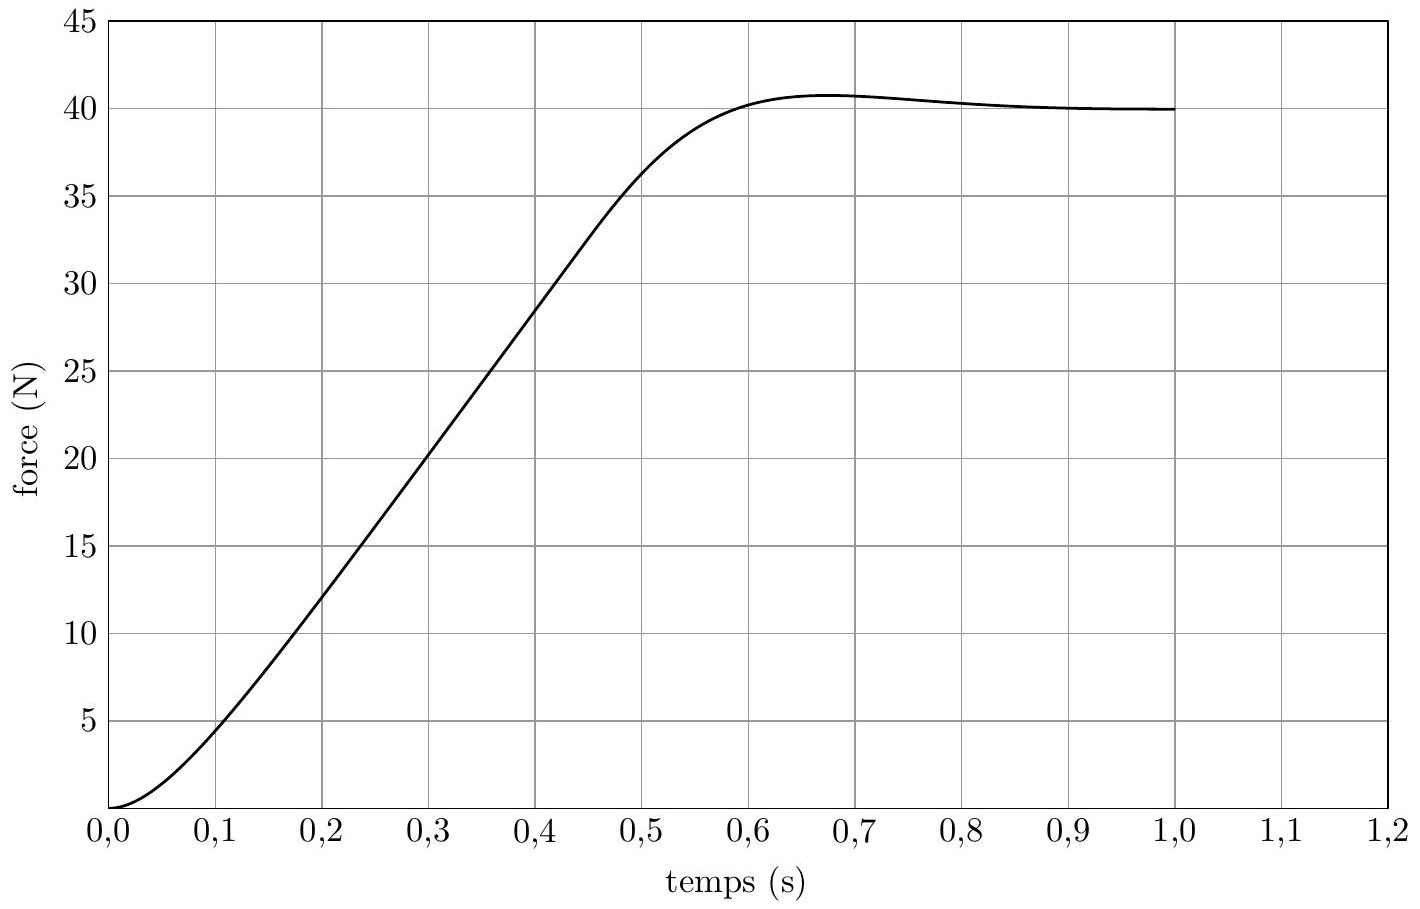
\includegraphics[width=\textwidth]{2025_09_16_5f2d7643f7e649c6833dg-14}
%\captionsetup{labelformat=empty}
%\caption{Figure 21 Réponse temporelle du modèle de connaissance pour une consigne de 40 N avec correction proportionnelle et limitation de la vitesse angulaire}
%\end{center}
%\end{figure}

\begin{figure}[!h]
\centering
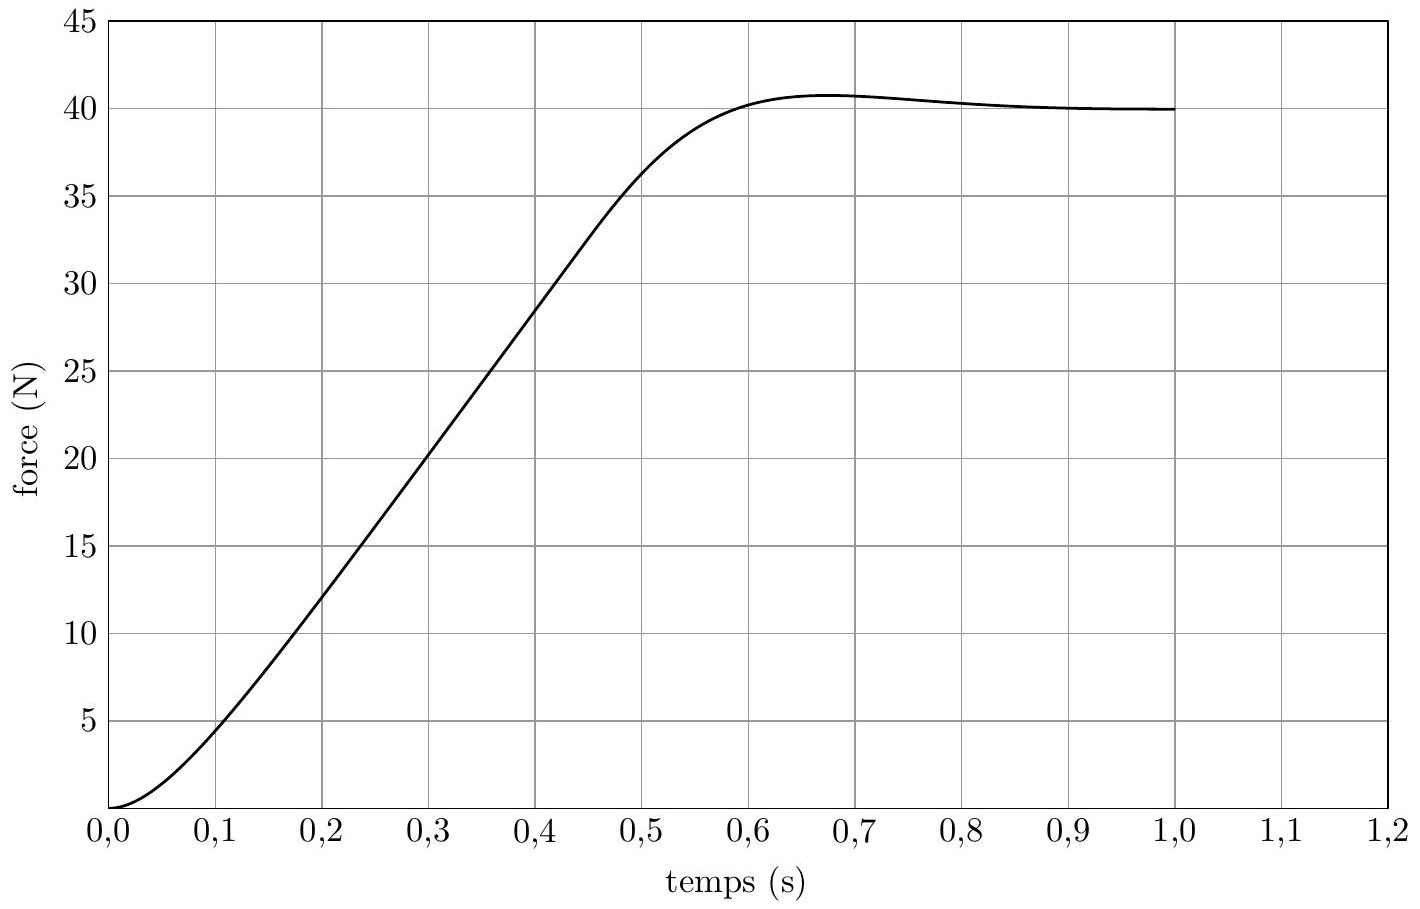
\includegraphics[width=.7\textwidth]{2025_09_16_5f2d7643f7e649c6833dg-14}
\caption{\label{ccs_mp_2023_fig_21}  Réponse temporelle du modèle de connaissance pour une consigne de 40 N avec correction proportionnelle et limitation de la vitesse angulaire}
\end{figure}



%Q 28. 
\question{\label{ccs_mp_2023_q_28}
Conclure sur la capacité du correcteur proportionnel avec limitation de la vitesse angulaire à respecter le cahier des charges, en analysant l'écart entre les performances simulées (figure \ref{ccs_mp_2023_fig_21}) et les performances attendues. Se limiter aux critères pertinents du tableau \ref{ccs_mp_2023_tab_05}.}
\ifprof
\begin{corrige}
\end{corrige}
\else
\fi



\section{Synthèse et ouverture de l'étude}
\begin{obj}
%Objectif}
Valider le modèle de connaissance, valider la commande optimisée et envisager un prolongement à l'étude.
\end{obj}

\subsection{Validation du modèle de connaissance et de la commande optimisée}%IV.A - 
On appelle commande optimisée la commande avec le correcteur de la boucle d'asservissement de force du type proportionnel avec limitation de la vitesse angulaire. Sur le banc d'essai avec l'actionneur linéaire, on implante ce correcteur, et on procède à quatre essais pour des consignes en échelon de force de $10,20,30$ et 40 N . Les mesures correspondantes sont tracées en traits discontinus sur la figure \ref{ccs_mp_2023_fig_22}. Ce même correcteur est mis en place dans le modèle de connaissance de la figure \ref{ccs_mp_2023_fig_11}, on obtient les réponses temporelles de simulation tracées en traits continus sur la figure \ref{ccs_mp_2023_fig_22}.

%\begin{figure}[h]
%\begin{center}
%  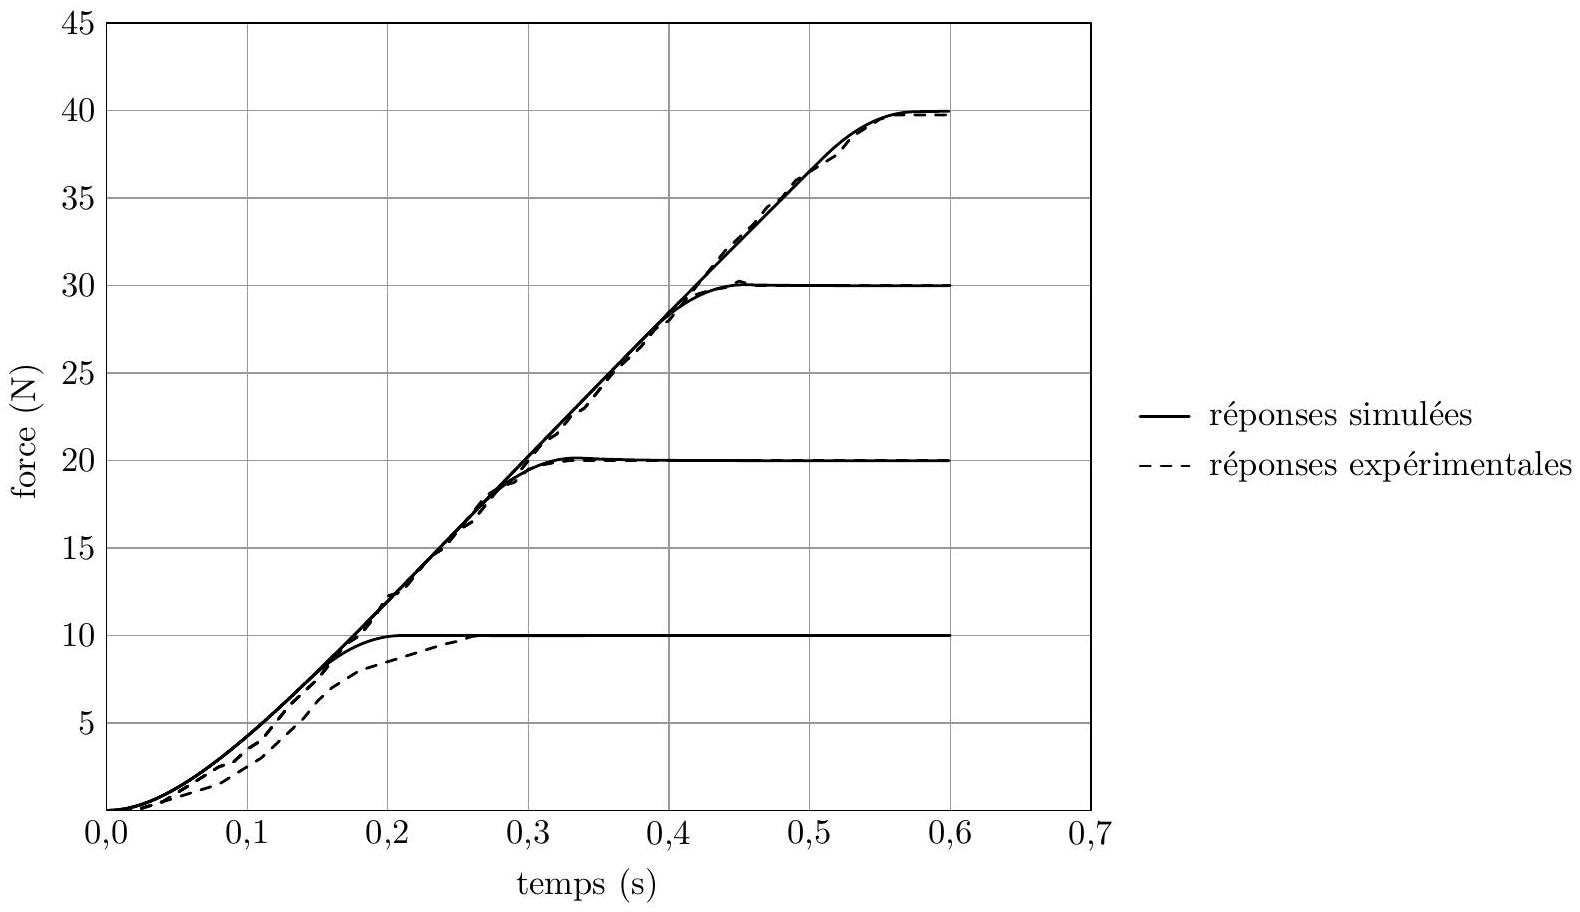
\includegraphics[width=\textwidth]{2025_09_16_5f2d7643f7e649c6833dg-15(1)}
%\captionsetup{labelformat=empty}
%\caption{Figure 22 Résultats des simulations et des expérimentations pour une entrée de consigne de force en échelon d'amplitude 10, 20,30 et 40 N}
%\end{center}
%\end{figure}

\begin{figure}[!h]
\centering
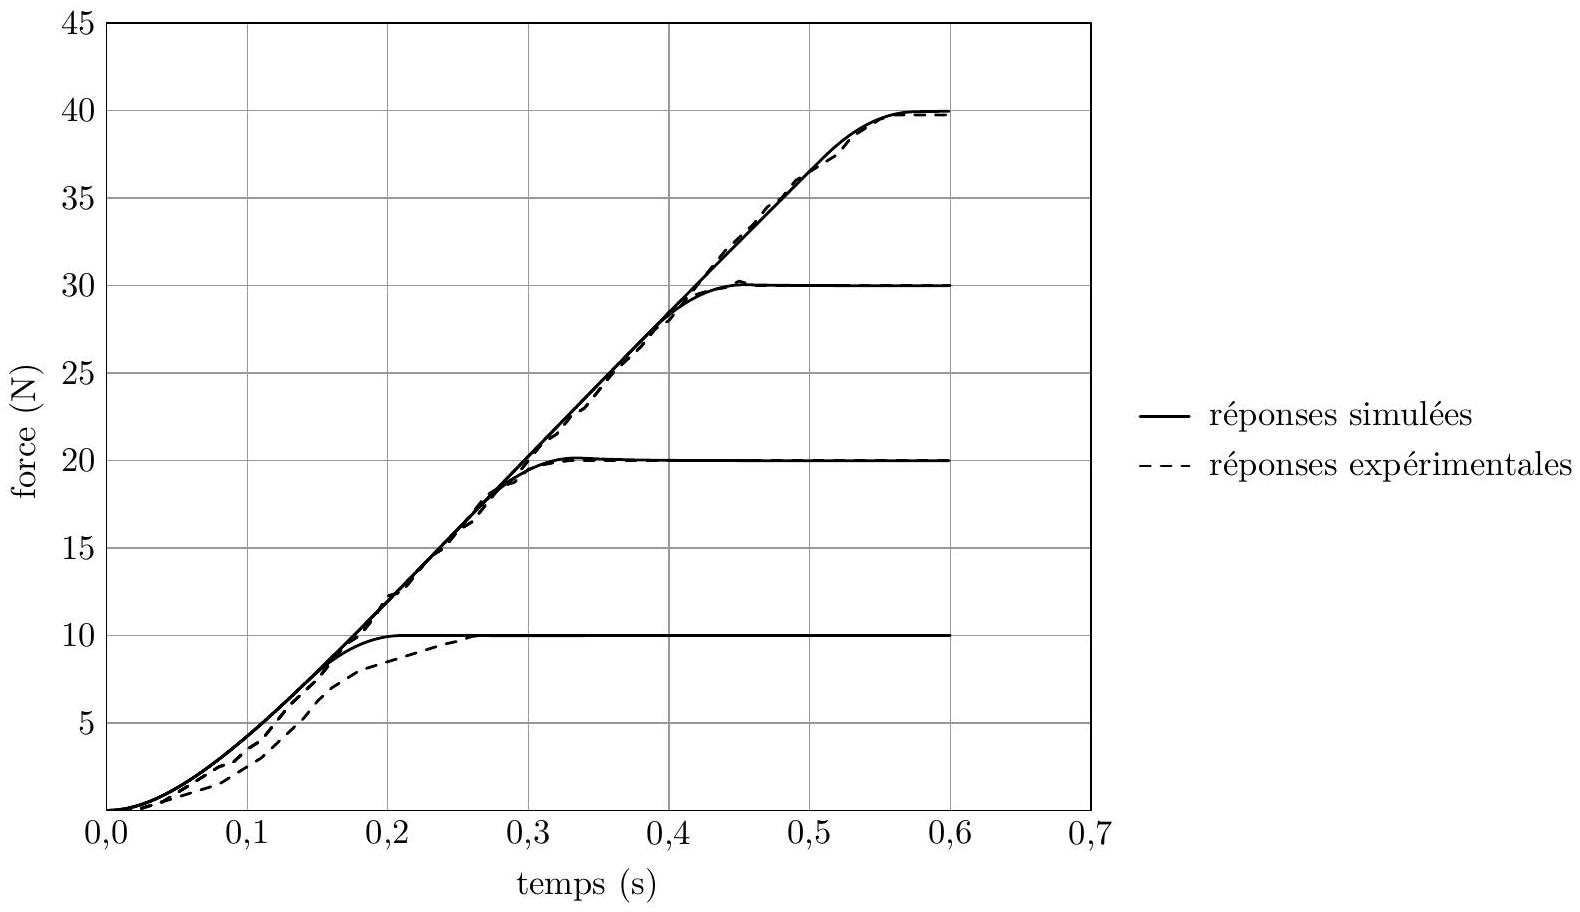
\includegraphics[width=.7\textwidth]{2025_09_16_5f2d7643f7e649c6833dg-15(1)}
\caption{\label{ccs_mp_2023_fig_22}   Résultats des simulations et des expérimentations pour une entrée de consigne de force en échelon d'amplitude 10, 20,30 et \SI{40}{N}}
\end{figure}



La démarche de l'ingénieur abordée dans le programme de sciences industrielles de l'ingénieur de la filière MP s'appuie sur les écarts entre trois performances (figure \ref{ccs_mp_2023_fig_23}).

%\begin{figure}[h]
%\begin{center}
%  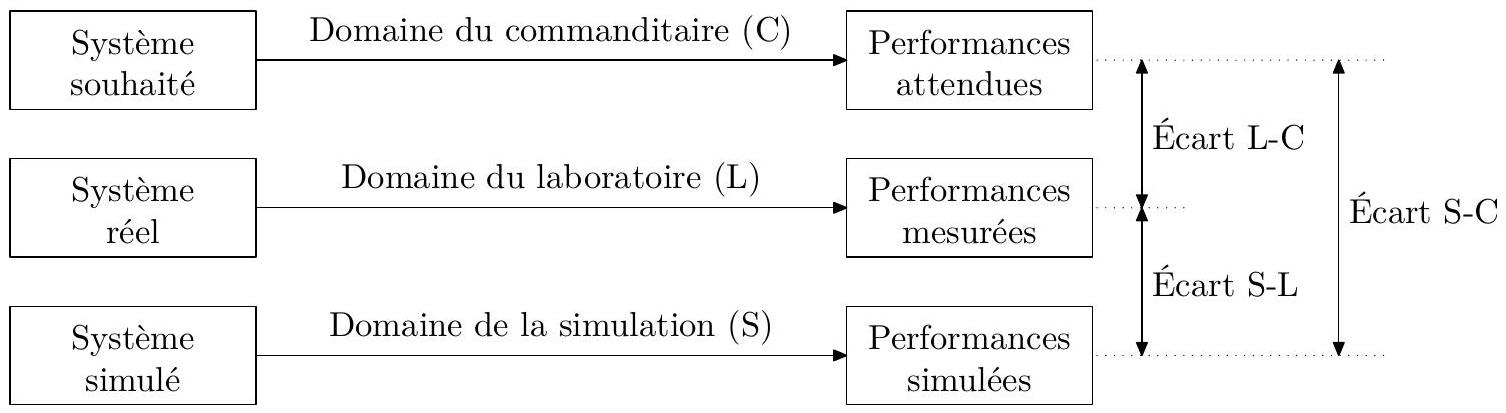
\includegraphics[width=\textwidth]{2025_09_16_5f2d7643f7e649c6833dg-15}
%\captionsetup{labelformat=empty}
%\caption{Figure 23 Synoptique de la démarche de l'ingénieur, telle que présentée dans le programme}
%\end{center}
%\end{figure}


\begin{figure}[!h]
\centering
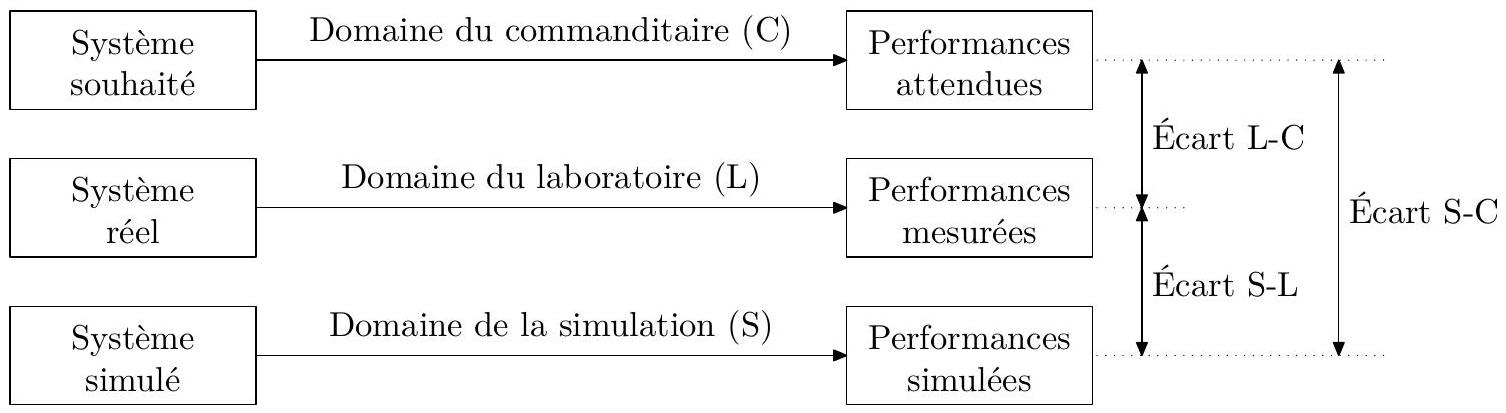
\includegraphics[width=\textwidth]{2025_09_16_5f2d7643f7e649c6833dg-15}
\caption{\label{ccs_mp_2023_fig_23}Synoptique de la démarche de l'ingénieur, telle que présentée dans le programme}
\end{figure}


En se référant à la figure \ref{ccs_mp_2023_fig_22}, l'analyse de l'écart entre les performances simulées et les performances mesurées valide le modèle de connaissance de l'asservissement de force.\\

%Q 29. 
\question{\label{ccs_mp_2023_q_29}
Choisir un des écarts L-C, S-L ou S-C permettant de valider la commande optimisée. Effectuer l'analyse de cet écart. Il est attendu une argumentation rigoureuse s'appuyant sur les données et les références du texte. Les numéros de figure, de tableau, ou d'exigence sont, par exemple, des références utilisables.}
\ifprof
\begin{corrige}
\end{corrige}
\else
\fi


\subsection{Étude du système perturbé}%IV.B - 
Le schéma-blocs de la figure \ref{ccs_mp_2023_fig_24} introduit une perturbation $Y_{\text {pert }}(p)$, représentant une perturbation dans le domaine temporel $y_{\text {pert }}(t)$.

%\begin{figure}[h]
%\begin{center}
%  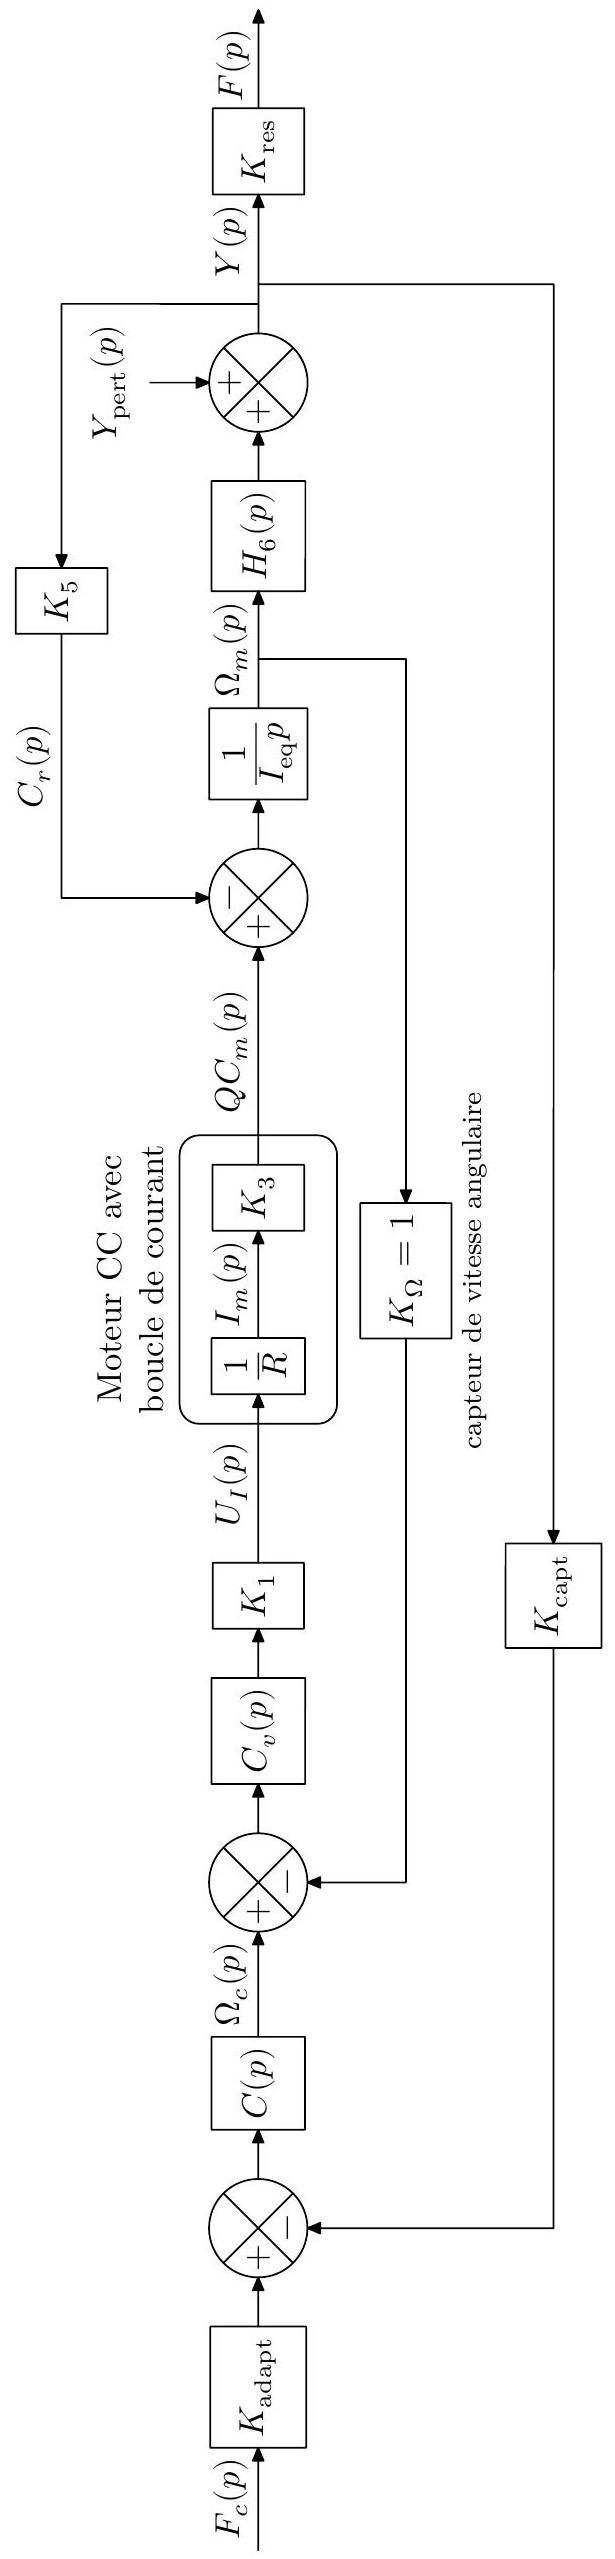
\includegraphics[width=\textwidth]{2025_09_16_5f2d7643f7e649c6833dg-16}
%\captionsetup{labelformat=empty}
%\caption{Figure 24 Schéma-blocs de l'asservissement de force développée par un actionneur linéaire avec perturbation}
%\end{center}
%\end{figure}


\begin{figure}[!h]
\centering
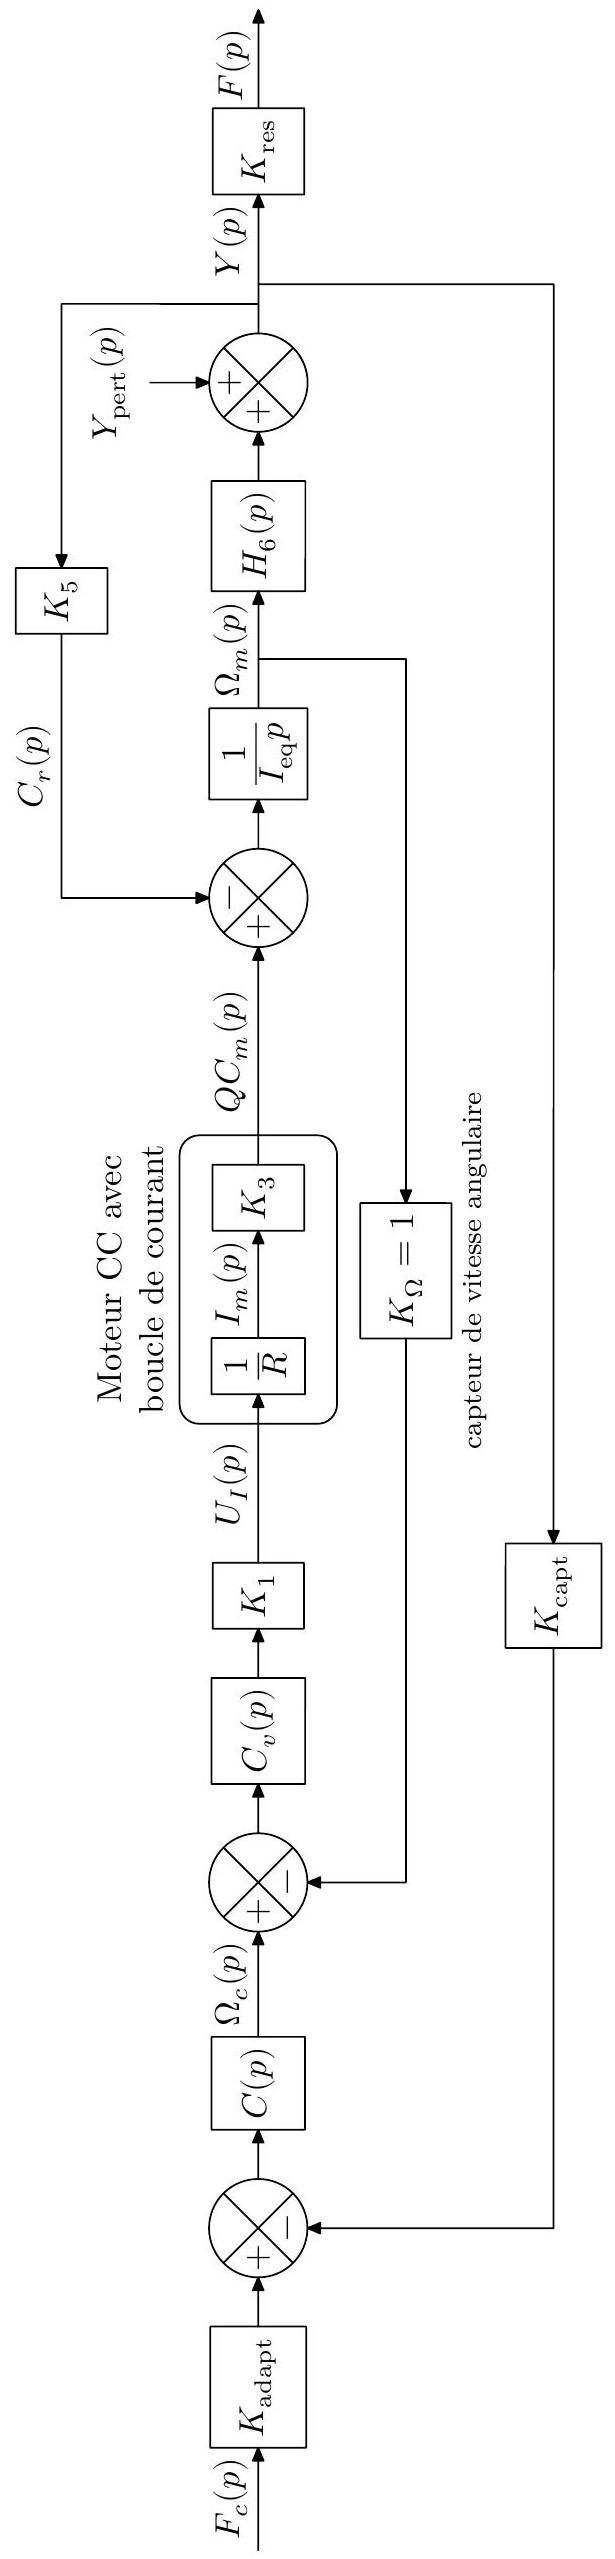
\includegraphics[width=.35\textwidth]{2025_09_16_5f2d7643f7e649c6833dg-16}
\caption{\label{ccs_mp_2023_fig_24}  Schéma-blocs de l'asservissement de force développée par un actionneur linéaire avec perturbation}
\end{figure}

%Q 30. 
\question{\label{ccs_mp_2023_q_30}
Quelle est l'unité de $y_{\text {pert}}(t)$ ? Que peut représenter cette perturbation dans le contexte de l'exosquelette lombaire? En se référant à la problématique du sujet, quel est l'intérêt d'introduire cette perturbation dans le modèle ?}
\ifprof
\begin{corrige}
\end{corrige}
\else
\fi

On effectue une simulation avec une perturbation normalisée représentée sur la figure \ref{ccs_mp_2023_fig_25}.

%\begin{figure}[h]
%\begin{center}
%  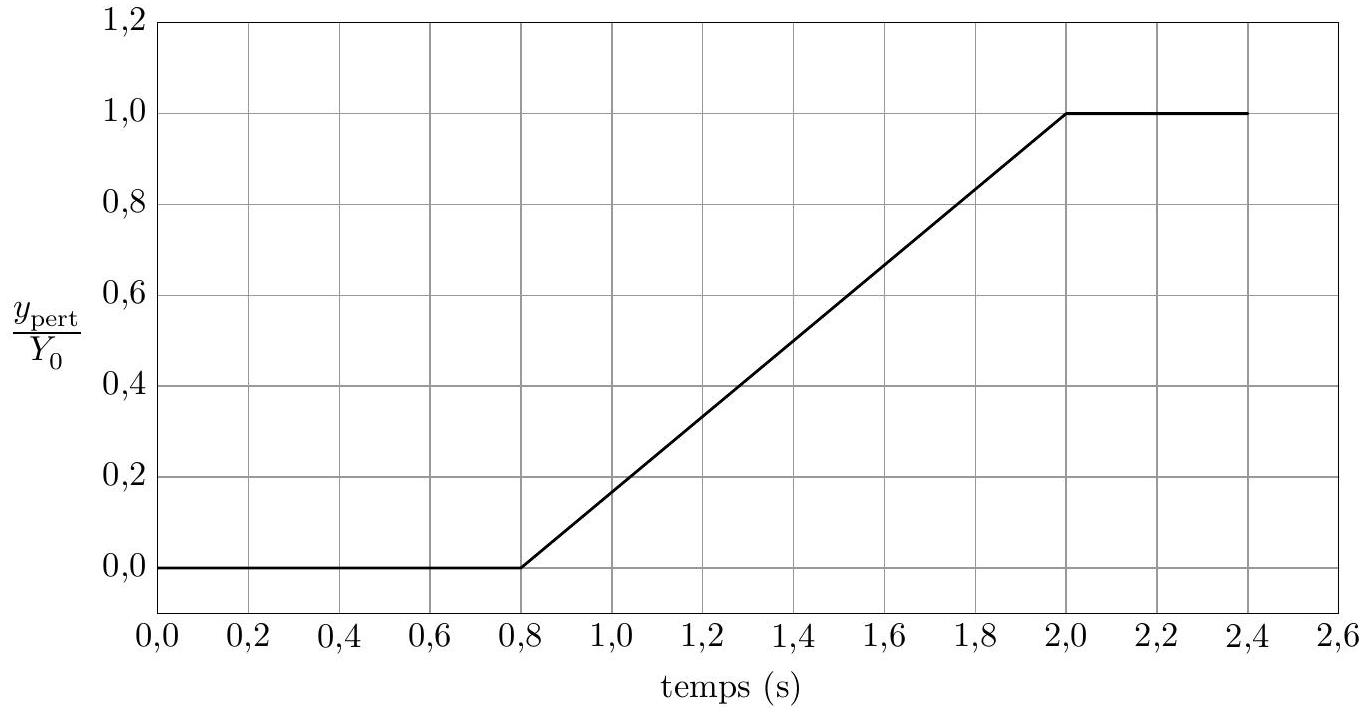
\includegraphics[width=\textwidth]{2025_09_16_5f2d7643f7e649c6833dg-17}
%\captionsetup{labelformat=empty}
%\caption{Figure 25 Évolution temporelle de la perturbation \$y\_\{\textbackslash text \{pert }\}(t)\$\}\end{center}
%\end{figure}

\begin{figure}[!h]
\centering
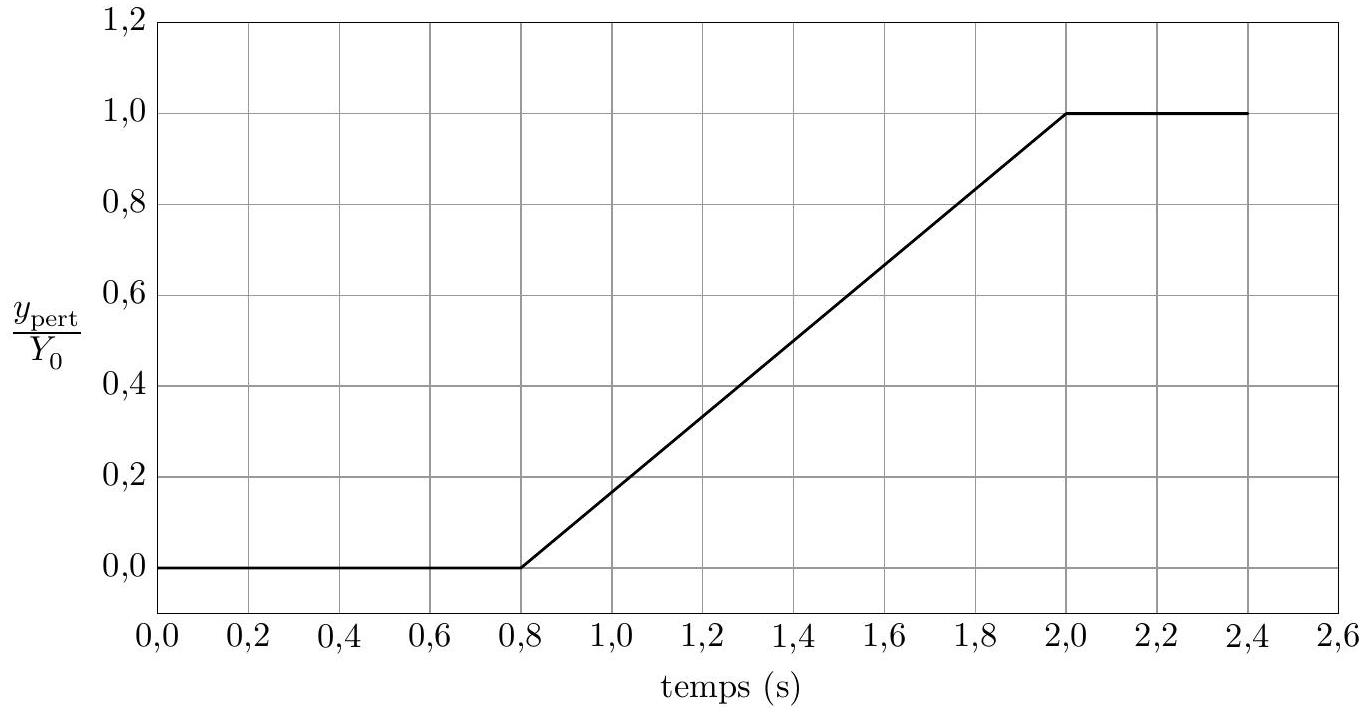
\includegraphics[width=.7\textwidth]{2025_09_16_5f2d7643f7e649c6833dg-17}
\caption{\label{ccs_mp_2023_fig_25}  Évolution temporelle de la perturbation $\indice{y}{pert}(t)$.}

\end{figure}



La figure 26 montre l'évolution de la force développée par un actionneur linéaire soumis à la perturbation décrite sur la figure \ref{ccs_mp_2023_fig_25}. C'est le résultat d'une simulation obtenue à partir du modèle de connaissance avec le correcteur proportionnel et limitation sur la vitesse angulaire.
%
%\begin{figure}[h]
%\begin{center}
%  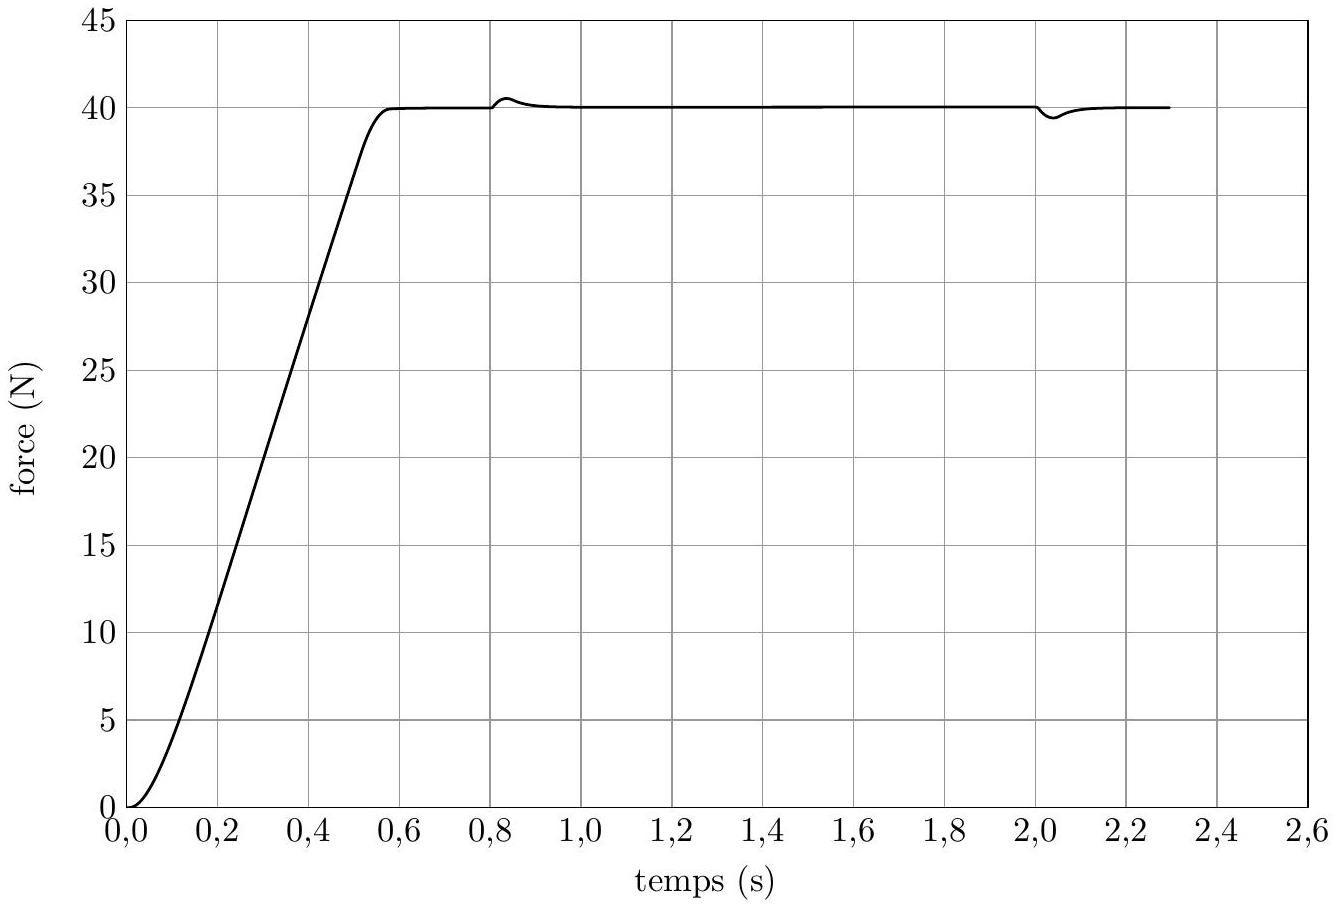
\includegraphics[width=\textwidth]{2025_09_16_5f2d7643f7e649c6833dg-17(1)}
%\captionsetup{labelformat=empty}
%\caption{Figure 26 Évolution de la force développée par l'actionneur linéaire soumis à une perturbation. Consigne en échelon de 40 N avec perturbation à \$t=0,8 \textbackslash mathrm\{\~{}s}\$\}\end{center}
%\end{figure}


\begin{figure}[!h]
\centering
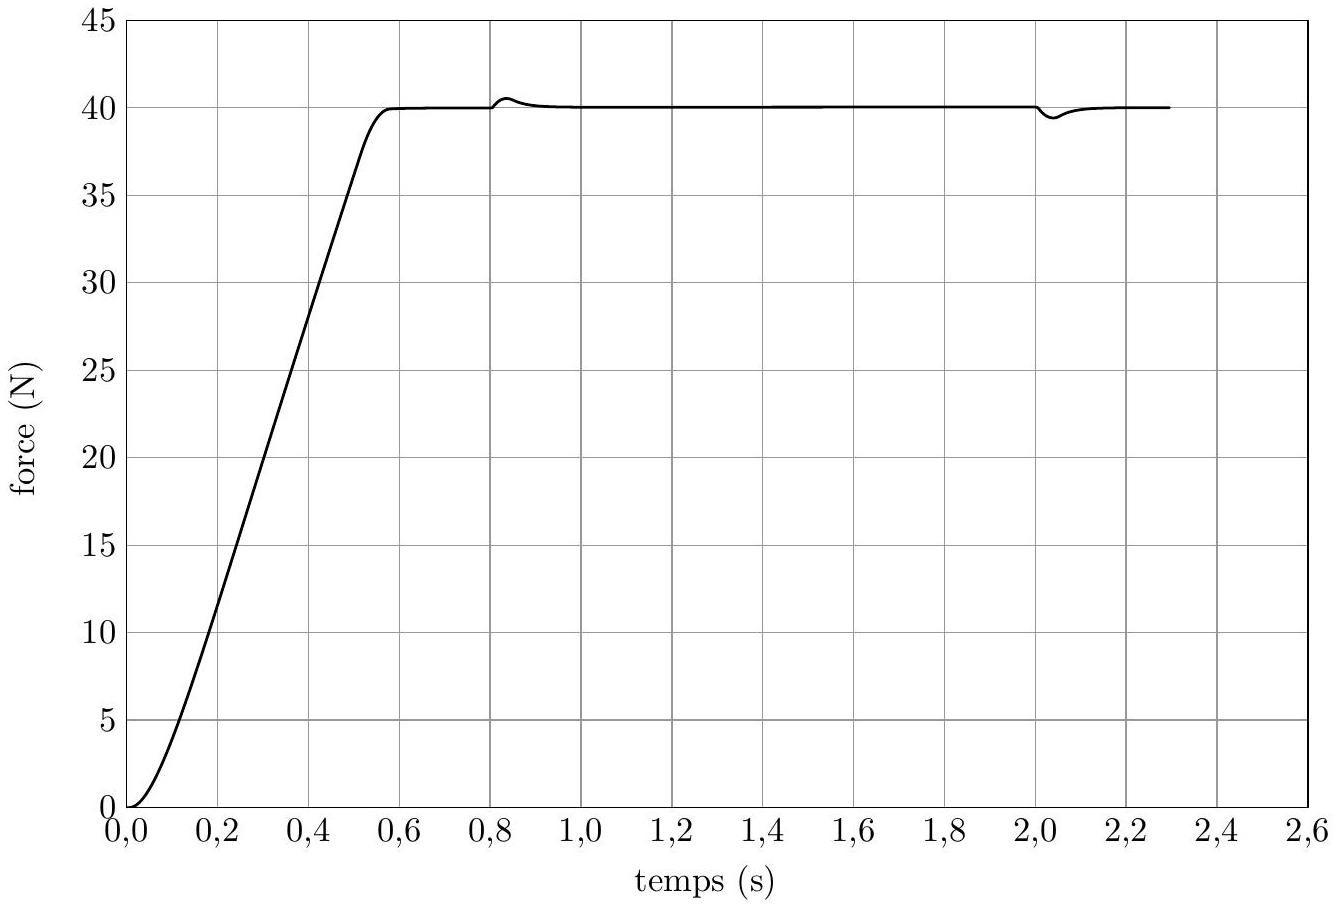
\includegraphics[width=.7\textwidth]{2025_09_16_5f2d7643f7e649c6833dg-17(1)}
\caption{\label{ccs_mp_2023_fig_}   Évolution de la force développée par l'actionneur linéaire soumis à une perturbation. Consigne en échelon de \SI{40}{N} avec perturbation à $t=\SI{0,8}{s}$.}

\end{figure}



%Q 31. 
\question{\label{ccs_mp_2023_q_31}
Analyser la courbe de simulation de la figure \ref{ccs_mp_2023_fig_26} et conclure au regard de la problématique du sujet.}
\ifprof
\begin{corrige}
\end{corrige}
\else
\fi


%Q 32.
\question{\label{ccs_mp_2023_q_32}
 Le banc d'essai équipé d'un actionneur linéaire, dans la configuration étudiée dans ce sujet, permet-t-il d'analyser l'écart S-L ?}
\ifprof
\begin{corrige}
\end{corrige}
\else
\fi

